\documentclass[11pt]{article}
\usepackage[a4paper,margin=2.6cm,headheight=14pt]{geometry}
\usepackage[T1]{fontenc}
\usepackage{lmodern}
\usepackage{microtype}
\usepackage{amsmath,amssymb,amsthm,mathtools}
\usepackage{booktabs,tabularx,longtable,array}
\usepackage{needspace}
\usepackage{enumitem}
\usepackage{xcolor}
\usepackage{listings}
\usepackage{fancyhdr}
\usepackage{caption}
\usepackage[hidelinks]{hyperref}
\usepackage[capitalise,nameinlink]{cleveref}
\usepackage{tikz}
\usetikzlibrary{positioning,arrows.meta,fit}

\definecolor{dcblue}{RGB}{28,58,92}
\definecolor{dcgray}{RGB}{246,246,246}
\definecolor{dcrule}{RGB}{190,190,190}
\hypersetup{colorlinks=true,linkcolor=dcblue,citecolor=dcblue,urlcolor=dcblue}
\hypersetup{pdftitle={Omega Memory and Goals in MeTTaDinC: A Practical Implementation Guide},
  pdfsubject={Implementation guide, Part I, 4 November 2026},
  pdfkeywords={MeTTaDinC, Omega, memory, goals, WMTM, GOLEM-Iter}}
\def\UrlBreaks{\do\/\do\_\do\.\do\-}
\newcommand{\fpath}[1]{\nolinkurl{#1}}

\lstdefinestyle{metta}{
  basicstyle=\ttfamily\small,
  backgroundcolor=\color{dcgray},
  frame=single, rulecolor=\color{dcrule}, framesep=4pt,
  columns=fullflexible, keepspaces=true,
  showstringspaces=false, breaklines=true,
  aboveskip=8pt, belowskip=8pt, xleftmargin=2pt, xrightmargin=2pt
}
\lstdefinestyle{mettafull}{
  style=metta, basicstyle=\ttfamily\scriptsize,
  numbers=left, numberstyle=\tiny\color{gray}, numbersep=6pt, xleftmargin=14pt,
  breakatwhitespace=true, postbreak=\mbox{\textcolor{gray}{$\hookrightarrow$}\space}
}
\lstdefinestyle{mettamod}{style=metta, basicstyle=\ttfamily\footnotesize}
\lstset{style=metta}

\newcommand{\code}[1]{\texttt{#1}}
\newcommand{\TV}{\operatorname{TV}}
\newcommand{\Q}{\mathbb{Q}}
\newcommand{\F}{\mathbb{F}}
\newcommand{\dnow}{\delta_{\mathrm{now}}}
\newcommand{\dupd}{\delta_{\mathrm{upd}}}
\newcommand{\dbd}{\delta_{\mathrm{beh}}}
\newcommand{\dtr}{\delta_{\mathrm{tr}}}
\newcommand{\dbeh}{d_{\mathrm{beh}}}
\newcommand{\Pbeh}{P_{\mathrm{beh}}}
\newcommand{\plain}{\paragraph{In plain terms.}}
\newcommand{\spec}[1]{specification, Section~#1}
\newcommand{\Spec}[1]{Specification, Section~#1}

\theoremstyle{definition}
\newtheorem{definition}{Definition}[section]
\newtheorem{example}[definition]{Example}
\newtheorem{remark}[definition]{Remark}
\theoremstyle{plain}
\newtheorem{proposition}[definition]{Proposition}
\newtheorem{lemma}[definition]{Lemma}

\setlist{itemsep=2pt,topsep=4pt}
\setlength{\parskip}{3pt}
\setlength{\emergencystretch}{3em}

\pagestyle{fancy}
\fancyhf{}
\fancyhead[L]{\small MeTTaDinC}
\fancyhead[R]{\small Omega memory and goals, 4 November 2026}
\fancyfoot[C]{\small\thepage}
\renewcommand{\headrulewidth}{0.4pt}

\newcommand{\nchecks}{195}

\begin{document}

\hypersetup{pageanchor=false}
\begin{titlepage}
\thispagestyle{empty}
\vspace*{2.2cm}
{\color{dcblue}\large\scshape Implementation guide\par}
\vspace{1.4cm}
{\color{dcblue}\fontsize{28}{34}\selectfont\bfseries Omega Memory and Goals\par}
\vspace{0.3cm}
{\color{dcblue}\fontsize{28}{34}\selectfont\bfseries in MeTTaDinC\par}
\vspace{0.7cm}
{\LARGE\bfseries A Practical Implementation Guide\par}
\vspace{0.7cm}
{\large Working, medium-term and long-term memory, goal engines and goal change,\\ written as
declared machines whose claims an agent can check\par}
\vspace{1.6cm}
{\large Companion to the MeTTaDinC specification draft, the Cetta implementation guide\\ and
\emph{MeTTaDinC in Practice: Four Worked Examples}\par}
\vspace{0.4cm}
{4 November 2026\par}
\vspace{0.8cm}
{Developed from the d-calculus and Hyperseed project\par}
\vfill
\noindent\begin{minipage}{\textwidth}
\small
{\color{dcblue}\bfseries Scope.} How to give Omega agents a MeTTaDinC layer over their memory and
goal machinery: what the layer is, where it attaches to the live WMTM system, the planned OCO/2
runtime and the GOLEM-Iter promotion gate, and how an agent uses it to reason about what it keeps,
what it may forget, and how its goals and their changes bear on its memory. Eight patterns are
worked out in full, each with a MeTTaDinC module, the expected result of every request, and notes
for implementers. A staged rollout plan closes the guide.

\smallskip
{\color{dcblue}\bfseries Validation material.} The patterns ship as one bundle: the module file,
a registry patch for the forms this guide proposes, Python models of every pattern, a small
reference evaluator that rebuilds every machine from the module text, an exact-arithmetic oracle
that recomputes every result of the patterns and compares the module with the models ($\nchecks$
checks), and the static checker. Where this text and the bundle differ, the bundle is
authoritative. Nothing here describes a change already made to a running Omega system.
\end{minipage}
\end{titlepage}
\hypersetup{pageanchor=true}

\begin{abstract}
\noindent
An Omega agent makes memory decisions every cycle. It recalls notes from a journal into a working
memory of sixty items, chooses about fifteen hundred tokens of them for the language model, admits
a few conclusions from its reasoner, closes and ages open questions, and lets a goal engine propose
follow-ups from what remains open; the planned runtime adds explicit decisions about what to keep
resident, what to retain and what to admit as evidence. Each decision keeps some
distinctions and drops others, and each is right or wrong only relative to the queries that later
read memory: the reply writer, the goal engine, the reasoner, the agent's own commitments and
anchors. MeTTaDinC states such decisions as representations of declared machines and checks, for
each declared consumer, whether the representation still answers its queries now, after updates
and in all future behavior, returning a replayable witness when it does not. This guide applies
that to Omega's memory and goals. It proposes an architecture: a library of declarations kept
beside the stores, a registry of consumers with custody rules, a checker that runs in the
background, a certificate store keyed by interface digests, receipts attached to context blocks
and goal suggestions, and a small interface through which the agent can ask about its own memory.
Eight patterns are worked out. Two failures reported by the first live review of the goal engine,
stale items that stayed open and paraphrases that repeated, reappear as canonical witnesses in a
model of the engine: closing items by what a recall window shows reopens them as replies age out of
the window, and deduplication by person and topic suggests the same question twice.
Policies for choosing the context block are compared consumer by consumer. Consolidation of
evidence is checked against a contradiction probe, a dependence-aware evidence count and an
anchor's regeneration cues, reproducing the failure modes of GOLEM-Iter's migration use case and
the smallest memory that serves all three. Task checkpoints without read sets are shown to be
adequate today and wrong after a withdrawal. Goals are treated as observers on memory: each goal
set determines the coarsest memory that serves it, adding a goal resumes refinement instead of
restarting it, retiring one licenses consolidation, and a proposed change to a goal is sorted into
renaming, refinement, coarsening, migration, failed migration or change of content by checks
that keep apart the information a
goal's answers carry and the decisions they stand for, read through declared and protected
decoders; a negated goal carries exactly the information of the original and is caught as a change
of content. Conflicts between goals and a
prohibition are found as shortest runs; MetaMo's motivational principles are measured on a finite
model shaped after its operational equations; and a monitor on the goal engine's stale suggestions gives
an anytime-valid alarm.
\end{abstract}

\subsection*{How to read this guide}
Section~\ref{sec:intro} says what the guide is for. Section~\ref{sec:background} gives the
background a reader needs from five places: the live WMTM system, the planned OCO/2 runtime,
the goal machinery of GoalChainer, GOLEM-Iter and MetaMo, MeTTaDinC itself, and the d-calculus
results the guide puts to work. Section~\ref{sec:arch} describes the architecture of the MeTTaDinC
layer. Sections~\ref{sec:p1}--\ref{sec:p8} are the eight patterns; each opens with the problem as
it appears in Omega, gives the module, the results and their reading, and closes with notes for
implementers. Section~\ref{sec:integration} attaches the layer to the live system, the OCO/2
runtime and the GOLEM-Iter gate and describes the interface the agent itself uses.
Section~\ref{sec:rollout} is the rollout plan, and Section~\ref{sec:limits} the limits and open
problems. The appendices hold the module file, the registry patch, the record schemas and the
reproduction notes.

A reader who wants the practical content first can read Section~\ref{sec:arch}, then the opening
and implementation notes of each pattern, then Sections~\ref{sec:integration}
and~\ref{sec:rollout}. Paragraphs headed \emph{In plain terms} restate a technical result without
notation. References to ``the specification'' are to the MeTTaDinC specification draft
\cite{spec}, and to ``the worked examples'' to its companion \cite{worked}.

\clearpage
{\setlength{\parskip}{0pt}\tableofcontents}
\clearpage

\section{Introduction}\label{sec:intro}

The distinction calculus started from a simple question about minds: which distinctions does a
system keep, which does it let go, and relative to whom is that the right choice? A memory is a
standing answer to that question. So is a summary, a cache, a context window, a consolidation
rule, and, one level up, a goal, which singles out the distinctions the system is committed to
acting on. Omega agents now answer the question many times a minute, in code that is still being
revised as its builders learn what goes wrong. This guide is about giving those answers a
form the agent can check, and then letting the agent use the checks to reason about its own memory
and goals.

The occasion is concrete. The WMTM layer of the Omega agent on ProtoCosmo2 recalls notes into a
working memory, chooses what the language model sees, admits conclusions from a reasoner, and runs
a goal engine over the open questions it remembers \cite{wmtm}. The first live review of its goal
suggestions failed, in part for reasons that are, in hindsight, statements about distinctions: old
replies were missed, so settled questions stayed open, and paraphrases of one question were
suggested again. A planned reimplementation inside the Omega runtime introduces typed records,
three separate decisions about residency, retention and admission, task checkpoints and goal
contracts \cite{oco2}. GOLEM-Iter adds a promotion gate that must decide whether a new memory policy
endangers a protected goal \cite{golemspec}. MetaMo describes how motivational state should evolve
\cite{metamo1,metamo2}. Several of these documents ask, in their own words, for claims of the kind
MeTTaDinC was designed to state: that a compact view keeps what its users need, now and after the
next update; that a migration commutes with repair; that a goal change preserves the answers it
claims to preserve.

\subsection{What this guide provides}

The guide proposes a MeTTaDinC layer for Omega memory and goals and works it out in enough detail
to implement. The layer does not replace the journal, PeTTa memory, the OCO/2 records or the goal
engine. It sits beside them as a library of declarations: machines whose actions are the memory
operations Omega already performs, observers that are the queries its components ask, and
representations that are the compact views it builds. A checker runs the requests in the
background and stores the results under the digest of the interface they concern. Components
consult the results through receipts, the GOLEM-Iter gate consumes them as certificates, and the
agent reaches them through a small set of functions.

Eight patterns make this concrete:
\begin{enumerate}
\item open items and the goal engine: closing, deduplication and the age cap
  (Section~\ref{sec:p1});
\item choosing the context block from working memory (Section~\ref{sec:p2});
\item consolidating evidence without losing contradictions, evidence lineage or an anchor's cues,
  and migrating an anchor's schema (Section~\ref{sec:p3});
\item task checkpoints that survive a restart and a withdrawal (Section~\ref{sec:p4});
\item goals as observers on memory: what each goal needs remembered, adding and retiring goals,
  and sorting proposed goal changes (Section~\ref{sec:p5});
\item conflicts between goals and a prohibition (Section~\ref{sec:p6});
\item MetaMo's principles measured on an implemented motivational dynamics
  (Section~\ref{sec:p7});
\item a monitor that watches the goal engine on live data (Section~\ref{sec:p8}).
\end{enumerate}
Each pattern is a MeTTaDinC module with the expected result of every request, computed exactly.
The models are small on purpose. Each is a small model that reproduces the decision a component
makes and the failure it can suffer, and each comes with notes on how the same
declarations scale to the real system.

\subsection{Status}

This is a design with validated fixtures. The modules conform to the MeTTaDinC registry together
with the patches of the worked examples and one small patch of this guide; an oracle recomputes
every number and checks that the module text and the Python models give the same results. No
MeTTaDinC runtime exists yet, the OCO/2 runtime is itself a plan, and the live WMTM system is
described as its report, dated 21 October 2026 with updates to 26 October, describes it
\cite{wmtm}. The models of WMTM's components are
models of the mechanisms the review described. Before a check of such a model is allowed to gate
anything, the model has to be tied to the code by the conformance tests of
Section~\ref{sec:records}.

\section{Background}\label{sec:background}

\subsection{Memory in a live Omega agent}\label{sec:wmtm}

WMTM (Working Medium-Term Memory) is the memory and reasoning layer of the ProtoCosmo2 agent, which runs on the Iter loop \cite{wmtm}. On every user turn a context hook recalls relevant
notes from a long-term journal of about ten megabytes into a working memory of sixty items plus
admitted conclusions, ranks them, and puts about $1{,}500$ tokens of the best-ranked items into the
language model's prompt. In the background, new notes are parsed into PLN atoms by a language-model
parser; PeTTaChainer reasons over the top items and admits at most five conclusions per cycle, each
with strength at least $0.5$, without writing anything derived back to the journal; and a goal
engine built on GoalChainer v2 turns open questions and pending items into proposals. The goal
engine weighs three needs (uncertainty, competence, and a legitimacy veto), closes items when it
sees a reply, ignores items older than seven days, and deduplicates proposals by person and topic.
Its proposals are logged, not shown, until a live review passes and the go-ahead to show them is
given. The report asks people to mark open items plainly (``open question for Ben: \ldots'',
``pending: \ldots'') and to close them plainly (``decided: \ldots''), because explicit markers are
what the engine reads.

The report is dated 21 October 2026, with updates to 26 October. Recall improved most: the share of the
right memories that reach the context rose from $30$ to $61$ percent, and the time WMTM adds to a
user turn fell from $8.6$ to $1.9$ seconds. Of twelve labelled conclusions the reasoner admitted,
four were correct, eight trivial and none wrong; the reasoner proves only one-step taxonomy,
because the memories are mostly the agent's own work logs. On replayed data the
share of goal proposals rated useful or plausible rose from $30$ to $80$ percent. The first live
review of goal suggestions, however, rated only $18$ percent useful or plausible, and the report
names the causes: stale items stayed open because old replies were missed, paraphrases repeated,
and some text was garbled. Fixes followed. Every feature sits behind a flag that is read each
cycle, every reasoner and goal run must pass a known-answer canary, and the report lists as a risk
that the agent runs as the same Linux user as its flags file and could change its own flags.

\subsection{The planned runtime}\label{sec:oco2}

A plan of 2 October 2026 reimplements WMTM inside the Omega runtime around the Omega Core
Ontology, version 2 (OCO/2) \cite{oco2}. It is a design with acceptance obligations; it claims no
implemented runtime. Several of its decisions bear directly on this guide.

\emph{Working memory as a record.} A \code{WorkspaceSnapshot} stores the selection policy, the time
of evaluation, each entry's attention, the decay anchor, use references, leases, omissions,
missing obligations and measured size, and ``the reason an item is active must be reconstructible
from these records.'' Selection includes task anchors (the current input and the task and goal
contracts) and bounded residency leases first, then uses goal relevance, attention and any declared
exploration policy; if mandatory material overflows the budget the result is blocked
or reported as quota-exceeded, never silently evicted.

\emph{Three decisions.} ``Residency, retention and admission are three decisions'': a residency
lease holds an item in the bounded active view, durable retention keeps a needed dependency
recoverable, and admission decides whether a route is eligible as evidence.

\emph{Task state.} A \code{Task} owns stable goals and constraints, and a \code{TaskCheckpoint}
records hypotheses, compatibility, pending queries, frontiers, plans, completed work and a read
set. A correct restart recovers ``which goal is active, why the leading hypothesis is being
investigated, which test is pending, which work already completed, and which previously valid
result now needs revalidation.''

\emph{Goals.} A \code{Goal} owns its target bindings, one tagged success specification, a verifier
and evidence requirements. Satisfaction is an event on the same immutable goal contract; a new
target, threshold or checker is a new contract; an invalidated supporting result reopens the goal.

\emph{Where the code goes.} The memory reducer, task and goal closure and the verifier are planned
in Python, and the logical ports are host-side: \code{admit\_bundle}, \code{validate\_current},
\code{select\_workspace}, \code{reason}, \code{record\_use}, \code{checkpoint},
\code{evaluate\_goal} and others. MeTTa holds inert cognitive structures and native operations.
The plan adds native binding queries over OCO records and asks that use, decay, retention and
ongoing work be explained from the records. It has no way to state or check claims about a memory
policy itself, such as which queries a retention rule preserves or what forgetting an item would
cost, and it specifies neither a self-model nor a learned memory policy. A companion plan for Iter's memory expects that an agent ``may
eventually reason about why it selected a premise or spent resources on an inference'' and asks
for policy versions and decision traces to be available as atoms \cite{itermem}.

The OCO/2 plan already contains, case by case, claims of the kind MeTTaDinC states in general. A count
fixture ``tests future-merge identity conservation, not just transport'': two origin sets
$\{a^+,b^-\}$ and $\{c^+,d^-\}$ with prior $(1,1)$ have the same mean $1/2$, but merging $\{a^+\}$
leaves the first at $1/2$, since $a^+$ is already in it, and moves the second to $3/5$. The lane for external ontologies asks implementers to ``check
source/receiver context and future-update preservation, not only current display equivalence,''
and reasoner wrappers must state ``explicit losses.''

\subsection{Goals in Omega}\label{sec:goals}

\emph{GoalChainer} combines semantic perception, deontic reasoning over defeasible norms
(forbidden, permitted, obligated), PLN and subjective-logic evidence with provenance, MetaMo
reconciliation and directive generation. It is too slow to run on every fast Iter step
\cite{golemspec}.

\emph{GOLEM-Iter} combines the GOLEM meta-architecture \cite{golem} with Iter
\cite{golemspec,golemformal}. A Searcher proposes changes to the agent's surface, a fixed Tester
evaluates them, a goal evaluator built on GoalChainer judges them, and a promotion gate answers each
proposal with promote, shadow, reject or escalate. Every candidate is classified by its maximum
plausible authority: A0 for a pure helper, A1 for a reversible workspace tool or context
transform that touches no anchor, A2 for a persistent memory policy, channel ingress or broad
context transform, A3 for privileged operations, evaluator approximations and changes at an
anchor's boundary, and A4 for constitutional norms, anchor identity, probes, rankings and gate
policy, which need an external ceremony. Memory is governed by class: raw observations, beliefs,
summaries and retrieval indexes, operator instructions, procedural strategies, anchor cues, norm
and probe definitions, and secrets each have their own policy. A note about a codebase, a persistent
prompt fragment and a memory file that supports an anchor are all writes to memory, and treating
them alike ``would be a category error.'' Deleting or consolidating an anchor cue requires an
anchor-margin analysis. An \emph{anchor} is a protected functional goal together with the cues and
repair rules from which the agent's ordinary dynamics regrow it after damage, a probe battery that
tests whether the regrown goal still controls behavior, and an evidence record.

GOLEM-Iter's first use case follows a hypothetical research hive, Meridian, that compresses its
episodic memory and migrates its evaluation core. Closed-loop replay finds that the compressed context drops
minority contradictory evidence. A learned evaluator gains unjustified confidence from
near-duplicate judgments of one incident. After a rename, a lesion rehearsal regrows the
verification goal pointing at the old policy name, ``a sentence on the wall.'' And compression
removes most of the raw incidents from which the verification commitment was historically
re-derived, so regenerative depth falls below its floor; the repair keeps ``a small, diverse,
provenance-bearing set of integrity incidents outside lossy compression'' and adds a second,
independent cue pathway. Pattern~3 reproduces these four failures in a model small enough to check
exhaustively.

\emph{MetaMo} describes motivational dynamics with an appraisal step $\Psi$ that updates
modulators and a decision step $D$ that updates goal weights, composed as $F=D\circ\Psi$
\cite{metamo1}. It asks that swapping the order of appraisal and decision change little, that $F$
contract near the boundary of a safe region, and that updates blend gradually toward preferred
states. Its mapping to OpenPsi and MAGUS gives a goal vector with two overgoals, individuation and
transcendence, six modulators, and a safe region in which the individuation weight stays above a
threshold and the goal vector's norm stays bounded \cite{metamo2}. The papers argue that real
systems can manifest the principles approximately and give no procedure for checking whether an
implementation does; Pattern~7 supplies one for a finite model.

\subsection{MeTTaDinC in brief}\label{sec:mettadinc}

A MeTTaDinC \emph{machine} is a finite set of states, a list of \emph{actions} that change the state,
and a list of \emph{observers}, the queries a consumer asks. A \emph{representation} encodes each
state as a code: a summary, a cache key, a selected context, a checkpoint. The specification gives
a representation three separate obligations \cite[Section~4.2]{spec}.

\emph{Now.} Two states with the same code give the same answer to every query. Then the code
can be used as an index.

\emph{Updates.} Two states with the same code have successors with the same code under every
action. Then a memory that keeps only the codes can maintain them by itself, which is what it
means for a memory to run on its codes.

\emph{Behavior.} Two states with the same code give the same answers after every sequence of
actions. Then the code predicts the future answers, which is what an index or summary used over
time needs.

\code{CheckNow}, \code{CheckUpdates} and \code{CheckBehavioral} answer these with a status. Checked
means the claim is established within its scope, either by an exact method that the core runs on
the declared model, such as finite enumeration in exact arithmetic or partition refinement, or by
a certificate that the core's replay checker validates. A verdict that rests on an external
solver's answer which the core has not replayed, such as an SMT solver's report that a formula has
no solution, is Conditional: it carries its undischarged assumption, written with the solver, its
version, the logic and the digest of the obligation, for example
\code{(TrustedBackend cvc5 1.4.2 QF\_LRA sha256:...)}. Every Checked result in this guide comes
from exact finite enumeration in rational arithmetic, so it is Checked under this policy and
carries no assumptions. Refuted comes with a replayable witness, and the canonical witness is the
least one: shortest word first, then pairs in the order of the carrier's declaration, then actions
and queries in declaration order. Unknown means a budget ran out and is never reported as anything
else; Estimated is reserved for statistical claims about data.
\code{MinimizeForQueries} returns the coarsest partition of the states that preserves every
query now and after every update. It is the smallest memory that serves the declared consumers,
and its classes say what may be forgotten. A \code{BlockPartition} checked on a carrier of
reachable states proves a safety property or returns the shortest run that violates it. An
\code{AbstractionMap} between two machines is checked for commuting with every action and
preserving every query. An \code{Implementation} contract bounds how far an implementation can
stray from an ideal, $d(\hat f(\hat x),f(x))\le L\,d(\hat x,x)+\eta$ over audited pairs. Monitors
watch recorded streams and report Estimated detections with Ville's inequality behind them
\cite{worked}.

Two facts from the specification are used throughout. First, results transport across interface
changes: when a query is added, existing results for the old queries stand and refinement resumes
from the current partition; when a query is removed, adequacy results transport but a ``coarsest''
result weakens to ``sufficient'' \cite[Section~4.8]{spec}. Second, the worked examples showed that
``store the belief in fewer bits'' can mean three things with three different claims: an index or
summary (behavioral), cold storage that is rehydrated to a representative (each cycle of storing and
restoring adds at most one radius of error), and a memory that runs on its codes (an arrow defect
that compounds with every update) \cite[Section~3.7]{worked}. WMTM uses all three at once: the context block is an
index, consolidation followed by recall is cold storage, and a working memory that reasons over
parsed atoms and admitted conclusions runs on its codes.

\subsection{The d-calculus results put to work}\label{sec:dcalc}

Three recent d-calculus papers bear directly on memory and goals, and their central finite
results fit together.

The goal-preservation paper defines a goal observer as a family of answers to labelled comparison
queries and calls two implementation states goal-equivalent when every finite sequence of updates
leaves their goal answers equal. Its Theorem~4.2 states that on a finite deterministic system this
is the largest equivalence that preserves current goal responses and is closed under updates, that
partition refinement reaches it in at most $|S|-1$ strict refinements, and that every closed
goal-sufficient observer refines it; the section is titled ``An observer must retain what future
updates can expose'' \cite{goalpres}. The first part of the agent-self companion makes a family of
protected, executable consumers (capability, evidence, commitments, attribution, control,
continuity) the core of a self-model and shows that the consumers' joint answers give the coarsest
exact partition, so that ``their answer distinctions determine what a self-representation may
safely forget''; it adds that ``retention choices should state the surviving query contract and any
loss of replay scope'' \cite{self1}. The concept-formation paper proves that the coarsest
quotient preserving declared tests, costs, guards and continuation kernels preserves
finite-horizon optimal control (Theorem~4.1) \cite{concept}.

\code{MinimizeForQueries} carries out the computation behind the goal-preservation and
concept-formation results, applied to goal queries and to control queries. The agent-self result
concerns current answers only: it supplies the starting partition, the joint answers of the
self-model's consumers, which \code{MinimizeForQueries} then refines until it is closed under
updates. The papers also sketch record types for an implementation: goal contracts,
representation maps and rewrite proposals in the goal-preservation paper, and in the agent-self
paper a table of ten self-model record contracts that it calls ``a proposed interface, not tested
MeTTa syntax.'' This guide writes such
records as MeTTaDinC declarations that a checker can run.

\section{Architecture of the MeTTaDinC layer}\label{sec:arch}

\subsection{What the layer adds and what it leaves alone}

The layer adds statements about memory, never memory itself. The journal, PeTTa memory and the
OCO/2 records keep their single authoritative writers, the memory reducer keeps applying events,
the goal engine keeps proposing, and the gate keeps deciding. What is new is a set of declarations
that describe what those components do in terms a checker can test, a place to keep the results,
and a way for components and for the agent to read them. A component that ignores the layer
behaves as before; a component that reads it can refuse to act on a view whose adequacy for its
own queries is Refuted or Unknown.

\begin{figure}[ht]
\centering
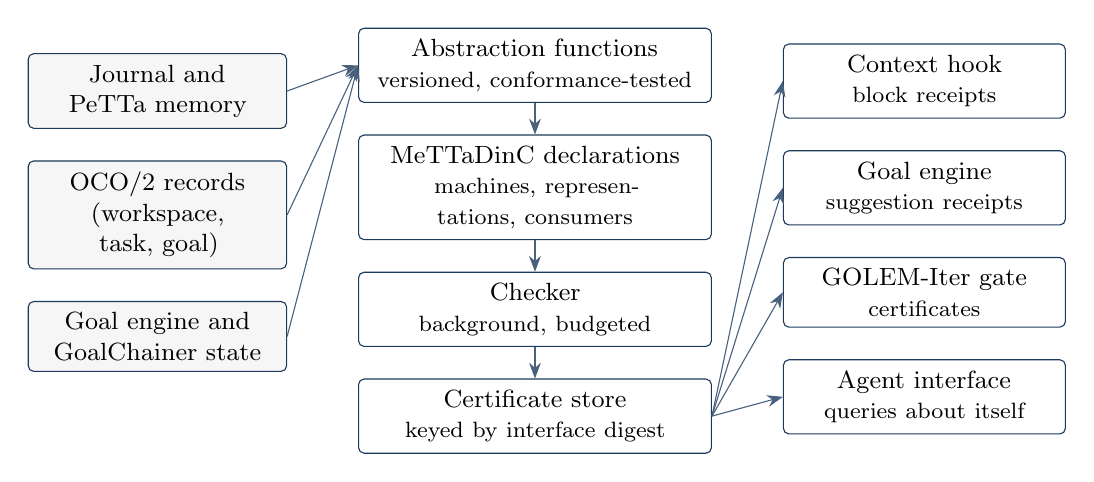
\begin{tikzpicture}[
  box/.style={draw=dcblue, rounded corners=2pt, align=center, font=\small, minimum height=8mm,
              inner sep=4pt, fill=white},
  store/.style={box, fill=dcgray, text width=3.0cm},
  mid/.style={box, text width=4.2cm},
  user/.style={box, text width=3.3cm},
  arr/.style={-{Stealth[length=2mm]}, draw=dcblue!80}]
\node[store] (j) {Journal and\\ PeTTa memory};
\node[store, below=4mm of j] (o) {OCO/2 records\\ (workspace, task, goal)};
\node[store, below=4mm of o] (g) {Goal engine and\\ GoalChainer state};
\node[mid, right=9mm of o, yshift=19mm] (a) {Abstraction functions\\ \footnotesize versioned, conformance-tested};
\node[mid, below=4mm of a] (d) {MeTTaDinC declarations\\ \footnotesize machines, representations, consumers};
\node[mid, below=4mm of d] (c) {Checker\\ \footnotesize background, budgeted};
\node[mid, below=4mm of c] (s) {Certificate store\\ \footnotesize keyed by interface digest};
\node[user, right=9mm of a, yshift=-2mm] (u1) {Context hook\\ \footnotesize block receipts};
\node[user, below=4mm of u1] (u2) {Goal engine\\ \footnotesize suggestion receipts};
\node[user, below=4mm of u2] (u3) {GOLEM-Iter gate\\ \footnotesize certificates};
\node[user, below=4mm of u3] (u4) {Agent interface\\ \footnotesize queries about itself};
\draw[arr] (j.east) -- (a.west);
\draw[arr] (o.east) -- (a.west);
\draw[arr] (g.east) -- (a.west);
\draw[arr] (a) -- (d);
\draw[arr] (d) -- (c);
\draw[arr] (c) -- (s);
\draw[arr] (s.east) -- (u1.west);
\draw[arr] (s.east) -- (u2.west);
\draw[arr] (s.east) -- (u3.west);
\draw[arr] (s.east) -- (u4.west);
\end{tikzpicture}
\caption{The MeTTaDinC layer beside Omega's memory and goal machinery. Arrows show the flow of
information; no arrow writes into the stores.}\label{fig:arch}
\end{figure}

\subsection{Components}

\paragraph{Declarations.} MeTTaDinC modules describe each memory component and each family of goals:
the machine (the states the component can be in, the actions that change them), the observers
(the queries its users ask), and the representations (the compact views it builds). Each
declaration has an interface identity, to which every result refers \cite{spec}; this guide
takes it to be the digest of the declaration's normalized text together with everything it
imports. Declarations are versioned with the code they describe.

\paragraph{Consumer registry.} A consumer is a declared user of a machine's answers. This guide
proposes a \code{Consumer} declaration that names the machine whose observers are the consumer's
queries, the statuses the consumer acts on, its custody and, for a goal, a decoder that says what
the goal's answers ask of the agent (Section~\ref{sec:classify}):
\begin{lstlisting}
(Consumer EngineQueries     (Of GoalEngine)
  (Accepts Checked (Conditional (TrustedBackend cvc5))) (Custody Agent))
(Consumer CommitmentQueries (Of Commitments) (Accepts Checked) (Custody Frame))
\end{lstlisting}
A consumer declared with \code{(Accepts Checked)} acts only on Checked results. The clause
\code{(Conditional (TrustedBackend cvc5))} of the engine's consumer also admits Conditional results
whose only undischarged assumptions are that the solver cvc5 answered correctly. An agent consumer
may name such solvers; a frame consumer accepts only Checked results unless the external ceremony
records otherwise. A frame consumer is held outside the agent's rewrite authority; an agent
consumer may be changed by a proposal that passes the gate (Section~\ref{sec:custody}).

\paragraph{Checker.} A worker runs requests against the declarations. It runs at idle priority,
like WMTM's other workers, under explicit budgets, and never on the user-turn path. A budget that
ends produces Unknown with a record of the work done.

\paragraph{Certificate store.} Results are stored with the request, the interface digest, the
digest of the model's abstraction functions, the digest of the code the model describes, the
digest of the registry and its patches, the status, the witness or certificate, and the budget
used. Each result also records its binding: the declarations it was computed from, the machine and
interface it was checked against, its scope, its assumptions and its assurance, which every
operation that consumes the result checks first (Appendix~\ref{app:store}). When an interface
changes, existing
results are reused only through the specification's transport rules \cite[Section~4.8]{spec}:
adding a query keeps old results for old queries and resumes refinement; removing one transports
adequacy but weakens ``coarsest'' to ``sufficient''; editing an action invalidates results that
depend on it.

\paragraph{Receipts.} Runtime artifacts carry small receipts: a context block records which
consumers it serves for the current snapshot and which policy certificates stand behind it; a goal
suggestion records the lifecycle claims about its item; a consolidation records which consumers'
claims it preserved. Appendix~\ref{app:records} gives the record schemas.

\paragraph{Agent interface.} A handful of functions lets the agent ask about its own memory and
goals: why an item is kept, what forgetting it would cost, what a goal needs remembered, how a
proposed goal change classifies, which goals conflict (Section~\ref{sec:agentapi}).

\subsection{Three ways to use a model}\label{sec:uses}

\Cref{tab:uses} separates three uses of the same declarations. They differ in what the claim is
about and in the status it can carry.

\begin{table}[ht]
\centering\small
\begin{tabularx}{\textwidth}{>{\raggedright\arraybackslash}p{2.9cm}>{\raggedright\arraybackslash}X>{\raggedright\arraybackslash}p{3.0cm}}
\toprule
Use & What is checked & Status\\
\midrule
Release-time policy checks & A finite model of a policy (closing, deduplication, selection,
consolidation, arbitration) over abstract kinds of items, checked exhaustively before a release
is deployed & Checked or Refuted, about the model\\
Runtime snapshot claims & The current memory, abstracted to a model state: which consumers the
selected view serves now and through a bounded number of updates & Checked or Refuted for this
snapshot; Unknown at budget\\
Stream claims & Recorded event streams, pinned by digest, against declared null and alternative
laws & Estimated\\
\bottomrule
\end{tabularx}
\caption{Three uses of the declarations.}\label{tab:uses}
\end{table}

The first use is the cheapest and comes first in the rollout. It catches design errors before
deployment: if the live engine closes items through a recall window, as Pattern~1 models it, the
failures of the first live review that the pattern reproduces would have been Refuted results at
release time. The second use turns checks into receipts that travel with the
artifacts components build. The third is the only way to make claims about the live system's
behavior over time, and its claims are statistical by construction.

\subsection{From live records to finite models}\label{sec:records}

A model is finite; Omega's memory is not. The bridge is an \emph{abstraction function} from live
records to model states: an open-item record maps to its age in days and the status of its closing
reply; a working-memory entry maps to its kind (fresh recall, open item for the current speaker,
anchor or commitment, other) and its recency rank; an evidence record maps to its source and
polarity. Three rules make the bridge trustworthy.

\emph{Policies read only declared attributes.} A selection, closing or consolidation policy is
written as a function of the attributes the abstraction function exposes. When this holds, a
result checked on the model holds for every memory whose records map to the model's states,
whatever else the records contain. When a policy reads something the model omits, the model is
too coarse, and the conformance tests below are designed to fail.

\emph{Abstraction functions are code under test.} They are versioned, their digests enter the
certificate store, and a change to one invalidates the results that used it.

\emph{Conformance is tested by replay.} For a corpus of recorded event logs, the live component and
the model are driven by the same events; after each event the abstraction of the live state must
equal the model's state, and the live component's decision must equal the model's. This is the
check the worked examples' reference evaluator performs between a module and its Python model
\cite[Appendix~C]{worked}, applied between a model and running code. Mutation tests in the style of
the OCO/2 plan, in which a deliberately broken component must fail a named assertion, show that the
conformance tests can detect a deviation \cite{oco2}. A model check gates a release or a
promotion only when conformance holds on the corpus; otherwise its result is reported as
conditional on the abstraction assumption.

\subsection{Consumers and custody}\label{sec:custody}

Consumer declarations decide what every check protects, so whoever can edit them can redefine
success. GOLEM-Iter already draws the line: probes, rankings and test seeds stay outside the
authority of the candidates they evaluate, and changing a probe is an A4 change that needs an
external ceremony \cite{golemspec}. Its formal model adds that a probe family the agent can inspect
before optimizing against it gives no uniform guarantee \cite{golemformal}. The goal-preservation
paper requires that a replacement checker be justified by the retained verification boundary
rather than by its own report \cite{goalpres}, and the specification lists the extension of
certificate transport to rewrites of the checker itself as an open problem
\cite[Section~16.5]{spec}. The layer adopts five rules.
\begin{enumerate}
\item Consumers that protect anchors, commitments, norms and probe batteries have
  \code{(Custody Frame)}. Their declarations live with the anchor's externally held package and
  change only through the A4 path. They accept only Checked results unless the external ceremony
  records otherwise.
\item Operational consumers, such as the goal engine's queries or the reply writer's, have
  \code{(Custody Agent)}. The agent may propose changes; a change is a candidate like any other and
  passes the gate with the certificates of Section~\ref{sec:gate}. An agent consumer may also
  accept Conditional results that rest on solvers it names.
\item The checker, the abstraction functions of frame consumers and the certificate store are part
  of the trusted closure: they are read-only to the agent and promoted only through the
  constitutional path.
\item The agent reads everything. Read access to declarations and results is what makes
  metacognition possible; write access is what custody restricts.
\item A goal's decoder, the map from its answers to the decisions they stand for, is part of its
  consumer's declaration and has that declaration's custody. The decoders of protected goals are
  therefore held by the frame, and the interpretation obligation of Section~\ref{sec:classify}
  compares an old and a new goal under meanings the agent cannot rewrite.
\end{enumerate}
The live WMTM report notes that the agent runs as the same Linux user as its flags file and could
change its own flags. The declarations and the certificate store need the separation that the flags
file does not yet have.

\subsection{What components do with each status}\label{sec:statuses}

Consumers declare the statuses they accept \cite[Section~2.7]{spec}. An exact consumer acts only
on Checked results and is declared with \code{(Accepts Checked)}. An empirical consumer may also
accept Estimated results under its own signature and is declared with
\code{(Accepts Checked Estimated)}; it also accepts a result derived from an estimate, which is
Conditional on \code{(EstimatedPremise} \emph{result-digest delta}\code{)}, the estimate's digest and
failure probability. Either declaration may end with one clause \code{(Conditional} \emph{entry
...}\code{)} whose entries are \code{(TrustedBackend} \emph{solver ...}\code{)}, which admits results
that rest on an unreplayed answer of a listed solver, and \code{(Assumption} \emph{name
...}\code{)}, which admits results that rest on an assumption carried by a listed declaration, such
as an imported kernel whose masses were estimated. A Conditional result is admitted only when every
one of its undischarged assumptions is covered, as in
\code{(Accepts Checked Estimated (Conditional (TrustedBackend cvc5) (Assumption StepModel)))}. The
rules below make the statuses operational.

\emph{Checked}: proceed, and attach a receipt that cites the result. A Conditional result is
treated in the same way by a consumer whose declaration accepts it, and the receipt records its
assumptions; for every other consumer it is treated as Unknown.

\emph{Refuted}: the witness is a concrete case. At release time it blocks the release or the
promotion until the policy or the model changes. At runtime the component takes its declared
fallback: the context block includes the protected item the witness names, the goal engine
withholds the suggestion, consolidation keeps the incident.

\emph{Unknown}: never treated as Checked. The component reports the condition, as the OCO/2 plan
requires for a budget that cannot hold mandatory material, and takes the same fallback as for
Refuted.

\emph{Estimated}: used only by empirical consumers, with its protocol, sample, guarantee and stream
digest.

\emph{Unsupported} and \emph{InvalidInput} are configuration errors and are reported as such.

\Cref{tab:map} lists where each Omega component meets a MeTTaDinC object, and which pattern works it
out.

\begin{table}[ht]
\centering\small
\begin{tabularx}{\textwidth}{>{\raggedright\arraybackslash}p{4.4cm}>{\raggedright\arraybackslash}X>{\raggedright\arraybackslash}p{1.3cm}}
\toprule
Omega component & MeTTaDinC object & Pattern\\
\midrule
Open items, closing, age cap, deduplication & Machine of item states; record designs as
representations; safety of deduplication as a block partition & 1\\
Working memory to context block & One representation per selection policy, one machine per
reader & 2\\
Consolidation, evidence lineage, anchor cues & Representations of an evidence memory checked for
three consumers; schema migration as an abstraction map & 3\\
Task checkpoints & Representations of task state checked for restart queries & 4\\
Goals and goal changes & Goals as observers; goal-sufficient memory by minimization; changes
sorted by informational checks and an interpretation obligation with declared decoders & 5\\
Arbitration between goals and norms & Block partitions on reachable states & 6\\
Motivational dynamics (MetaMo) & Block partitions and implementation contracts & 7\\
Goal engine on live data & Monitors on digest-pinned streams & 8\\
\bottomrule
\end{tabularx}
\caption{Where Omega's memory and goal components meet MeTTaDinC.}\label{tab:map}
\end{table}

\section{Pattern 1: open items and the goal engine}\label{sec:p1}

\subsection{The problem}

The goal engine reads open questions and pending items from memory, closes an item when it sees a
reply, stops considering items older than seven days, and deduplicates its proposals by person and
topic. Each of these is a memory decision. The first live review of the engine's suggestions
failed, among other reasons, because ``stale items stayed open (old replies were missed)'' and
``paraphrases repeated'' \cite{wmtm}. The report does not describe the mechanisms. The model below
takes the simplest ones consistent with what it reports: a reply missed because it has left the
engine's recall window, and paraphrases that receive different deduplication keys.
The width of the recall window and the matching rules are parameters of the model, to be confirmed
against the code by the conformance tests of Section~\ref{sec:records}.

\subsection{The model}

One item is described by its age in days, with $8$ standing for more than seven, and by the time
since its closing reply: \code{none}, or \code{d0}, \code{d1}, \code{d2}, or \code{d3} for three or
more days. A day passing is the action \code{tick}; the arrival of a closing reply is the action
\code{reply}, and the first reply counts. The goal engine asks \code{suggest}: is the item open and
at most seven days old? The agent's commitment record asks \code{open}: is the item still open?
From a new item with no reply, $39$ of the $45$ combinations are reachable.

Three record designs are compared. The \emph{window view} is what the engine believes when it
derives closure from what its recall window shows, with replies visible for two days. The
\emph{event view} records the closing as an event on the item. The \emph{capped view} applies the
seven-day cap to the record itself and drops older items.
\begin{lstlisting}[style=mettamod]
(DC.Module OpenItems
  (Profile Crisp)
  (Use NatArith Families)                              ; PROPOSED libraries
  (Carrier Age   (Of Nat) (Enum 0 1 2 3 4 5 6 7 8))      ; 8: more than seven days
  (Carrier Reply (Of Symbol) (Enum none d0 d1 d2 d3))    ; days since the reply; d3: 3+
  (Carrier Item  (Of (Tuple Nat Symbol)) (Product Age Reply))
  (Carrier Seen  (Of Symbol) (Enum open closed dropped)) ; as a record design shows it
  (Const start Item (Tuple 0 none))

  ;; how an item changes
  (Map later (From Reply) (To Reply) (Table (none none) (d0 d1) (d1 d2) (d2 d3) (d3 d3)))
  (Map tick (From Item) (To Item)
    (Cases ((Tuple $a $r) (Tuple (Min (Add $a 1) 8) (later $r)))))
  (Map on-reply (From Item) (To Item)
    (Cases ((Tuple $a $r) (Tuple $a (If (Eq $r none) d0 $r)))))

  ;; what its users ask
  (Map suggest (From Item) (To Bool) (Cases ((Tuple $a $r) (And (Eq $r none) (Le $a 7)))))
  (Map open    (From Item) (To Bool) (Cases ((Tuple $a $r) (Eq $r none))))

  (Machine ItemLife (States Item)
    (Observe suggest suggest) (Action tick tick) (Action reply on-reply))
  (Carrier Live (Of (Tuple Nat Symbol)) (Reach ItemLife (From start)))
  (Machine GoalEngine  (States Live) (Like ItemLife))              ; PROPOSED Like
  (Machine Commitments (States Live) (Observe open open)
    (ActionsOf ItemLife))                                          ; PROPOSED ActionsOf
  (Machine Both (States Live) (Observe suggest suggest) (Observe open open)
    (ActionsOf ItemLife))
  ;; PROPOSED Consumer; the agent consumer also accepts results that rest on cvc5
  (Consumer EngineQueries     (Of GoalEngine)
    (Accepts Checked (Conditional (TrustedBackend cvc5))) (Custody Agent))
  (Consumer CommitmentQueries (Of Commitments) (Accepts Checked) (Custody Frame))

  ;; what the engine believes through its recall window, and two record designs
  (Map in-window (From Reply) (To Bool)
    (Table (none False) (d0 True) (d1 True) (d2 True) (d3 False)))
  (Map window-view (From Item) (To (Tuple Nat Symbol))
    (Cases ((Tuple $a $r) (Tuple $a (If (in-window $r) closed open)))))
  (Map event-view (From Item) (To (Tuple Nat Symbol))
    (Cases ((Tuple $a $r) (Tuple $a (If (Eq $r none) open closed)))))
  (Map capped-view (From Item) (To (Tuple Nat Symbol))
    (Cases ((Tuple $a $r)
      (If (Eq $a 8) (Tuple 8 dropped) (Tuple $a (If (Eq $r none) open closed))))))
  (Representation WindowView (Of GoalEngine) (Encode window-view))
  (Representation EventView  (Of GoalEngine) (Encode event-view))
  (Representation CapForEngine      (Of GoalEngine)  (Encode capped-view))
  (Representation CapForCommitments (Of Commitments) (Encode capped-view))
  (Derive EngineMemory     (MinimizeForQueries GoalEngine))
  (Derive CommitmentMemory (MinimizeForQueries Commitments))
  (Derive JointMemory      (MinimizeForQueries Both)))
\end{lstlisting}
The requests:
\begin{lstlisting}[style=mettamod]
!(dc.run OpenItems (CheckNow WindowView))
!(dc.run OpenItems (CheckUpdates WindowView))
!(dc.run OpenItems (CheckBehavioral EventView))
!(dc.run OpenItems (CheckUpdates EventView))
!(dc.run OpenItems EngineMemory)
!(dc.run OpenItems CommitmentMemory)
!(dc.run OpenItems JointMemory)
!(dc.run OpenItems (CheckBehavioral CapForEngine))
!(dc.run OpenItems (CheckNow CapForCommitments))
\end{lstlisting}

\subsection{Results}

\begin{table}[ht]
\centering\small
\begin{tabularx}{\textwidth}{>{\raggedright\arraybackslash}p{4.6cm}>{\raggedright\arraybackslash}p{1.7cm}X}
\toprule
Request & Status & Witness or value\\
\midrule
\code{CheckNow WindowView} & Refuted & pair $(3,\code{none})$, $(3,\code{d3})$; \code{suggest}: true
against false\\
\code{CheckUpdates WindowView} & Refuted & pair $(2,\code{d0})$, $(2,\code{d2})$; action
\code{tick}; codes $(3,\code{closed})$ and $(3,\code{open})$\\
\code{CheckBehavioral EventView} & Checked & \\
\code{CheckUpdates EventView} & Checked & \\
\code{EngineMemory} & Checked & $9$ classes\\
\code{CommitmentMemory} & Checked & $2$ classes\\
\code{JointMemory} & Checked & $10$ classes\\
\code{CheckBehavioral CapForEngine} & Checked & \\
\code{CheckNow CapForCommitments} & Refuted & pair $(8,\code{none})$, $(8,\code{d0})$; \code{open}:
true against false\\
\bottomrule
\end{tabularx}
\caption{Results of the open-item module.}\label{tab:p1}
\end{table}

\paragraph{The window view is wrong today.} An item never answered and an item answered three or
more days ago look the same through a two-day window: both look open, and the engine suggests a
follow-up for a question that was settled. The result envelope:
\begin{lstlisting}
(Result (Status Refuted)
  (Claim (Kind Now) (Representation WindowView) (Of GoalEngine))
  (Evidence (Witness (WordWitness (Pair (Tuple 3 none) (Tuple 3 d3))
              (SameCode (Tuple 3 open)) (Word (Do)) (Query suggest)
              (Left True) (Right False)))))
\end{lstlisting}

\paragraph{It also cannot be maintained.} In the model, the update witness is the mechanism behind
``stale items stayed open.'' Two items that both look closed today, one answered today and one answered two days
ago, diverge after one day: the second reply leaves the window and the item appears to reopen.
Closure derived from what the window currently shows is not preserved by the passage of time, so
no amount of tuning the window fixes it; a wider window only moves the day on which items reopen.

\paragraph{Event-sourced closing passes all three obligations.} Recording the closing as an event
on the item when the reply arrives makes the view answer \code{suggest} now and forever, and makes
it maintainable by itself.

\paragraph{What the engine needs to remember.} \code{EngineMemory} has $9$ classes on the $39$
states: one for each age of an open item up to seven days, and one class for everything else. A
closed item and an open item more than seven days old are the same thing to the suggestion
consumer, because neither will ever be suggested again. The engine never needs the time since the
reply. The
event view keeps $18$ codes; ten of them, the nine ages of a closed item and the expired open item,
fall into a single class of \code{EngineMemory}.

\paragraph{The age cap belongs to the query, not to the record.} The commitment consumer needs only
whether the item is open ($2$ classes), and the joint memory has $10$: it separates the expired open
item from the closed one, because to the commitment record an unanswered week-old question is
still an open commitment. Applied to the engine's query, the seven-day cap loses nothing
(\code{CapForEngine} is Checked). Applied to the record, it forgets that the item is open
(\code{CapForCommitments} is Refuted). The agent-self companion makes the same point from the
other side: consolidation must not erase commitments early \cite{self2}.

\plain The goal engine should close items when the reply arrives, by writing that fact on the item,
and never infer closure from what it happens to see. For its own purposes it may forget almost
everything about an item except whether it is open and, if so, how old it is. The commitment record
must not forget that an item is open just because the engine stopped asking about it.

\subsection{Deduplication}\label{sec:dedupe}

The second failure concerns two notes that ask one question in different words. The model tracks
whether each paraphrase has arrived, which deduplication keys have been suggested, and how many
suggestions the question has received (capped at two). When topic labels differ, a person and
topic key gives the two paraphrases different keys; a question key, which requires paraphrase
linking, gives them one. The safety requirement, at most one suggestion per question, is a one-block
partition on the reachable states:
\begin{lstlisting}[style=mettamod]
(DC.Module SuggestionDedupe
  (Profile Crisp)
  (Use NatArith Families)
  (Carrier Flag   (Of Bool) (Enum False True))
  (Carrier Count  (Of Nat) (Enum 0 1 2))
  ;; (n1 received, n2 received, key k1 suggested, key k2 suggested,
  ;;  number of suggestions about the question)
  (Carrier Engine (Of (Tuple Bool Bool Bool Bool Nat))
    (Product Flag Flag Flag Flag Count))
  (Const start Engine (Tuple False False False False 0))
  (Map recv1 (From Engine) (To Engine)
    (Cases ((Tuple $r1 $r2 $s1 $s2 $c) (Tuple True $r2 $s1 $s2 $c))))
  (Map recv2 (From Engine) (To Engine)
    (Cases ((Tuple $r1 $r2 $s1 $s2 $c) (Tuple $r1 True $s1 $s2 $c))))
  ;; person+topic key: the paraphrases carry different topic labels, hence different keys
  (Map run-by-topic (From Engine) (To Engine)
    (Cases ((Tuple $r1 $r2 $s1 $s2 $c)
      (Tuple $r1 $r2 (Or $s1 $r1) (Or $s2 $r2)
        (Min 2 (Add $c (Add (If (And $r1 (Not $s1)) 1 0)
                            (If (And $r2 (Not $s2)) 1 0))))))))
  ;; question key: paraphrase linking gives both notes the key k1
  (Map run-by-question (From Engine) (To Engine)
    (Cases ((Tuple $r1 $r2 $s1 $s2 $c)
      (Tuple $r1 $r2 (Or $s1 (Or $r1 $r2)) $s2
        (Min 2 (Add $c (If (And (Or $r1 $r2) (Not $s1)) 1 0)))))))
  (Map count-of (From Engine) (To Nat) (Cases ((Tuple $r1 $r2 $s1 $s2 $c) $c)))
  (Map repeated (From Engine) (To Bool) (Body ($x) (Le 2 (count-of $x))))
  (Machine ByTopic (States Engine) (Observe repeated repeated)
    (Action recv1 recv1) (Action recv2 recv2) (Action run run-by-topic))
  (Machine ByQuestion (States Engine) (Observe repeated repeated)
    (Action recv1 recv1) (Action recv2 recv2) (Action run run-by-question))
  (Carrier LiveTopic    (Of (Tuple Bool Bool Bool Bool Nat))
    (Reach ByTopic (From start)))
  (Carrier LiveQuestion (Of (Tuple Bool Bool Bool Bool Nat))
    (Reach ByQuestion (From start)))
  (Machine TopicWatch    (States LiveTopic)    (Like ByTopic))
  (Machine QuestionWatch (States LiveQuestion) (Like ByQuestion))
  (BlockPartition OnceByTopic (On LiveTopic)
    (Block Once (Body ($x) (Le (count-of $x) 1)) start)
    (Successor Any Once Once))                                          ; PROPOSED Any
  (BlockPartition OnceByQuestion (On LiveQuestion)
    (Block Once (Body ($x) (Le (count-of $x) 1)) start)
    (Successor Any Once Once)))

!(dc.run SuggestionDedupe (CheckBlockPartition OnceByTopic (Of TopicWatch)))
!(dc.run SuggestionDedupe (CheckBlockPartition OnceByQuestion (Of QuestionWatch)))
\end{lstlisting}
With the person and topic key, $9$ states are reachable and \code{OnceByTopic} is Refuted with the
least word \code{(Do recv1 recv2 run)}: both paraphrases are open when the engine runs, and it
suggests the question twice. With the question key, \code{OnceByQuestion} is Checked on all $7$
reachable states. The repair moves the risk to paraphrase linking: the policy is correct whenever
linking is, and linking's accuracy is an empirical quantity that belongs in an Estimated claim on
a labelled sample or in a monitor (Section~\ref{sec:p8}).

\subsection{Notes for implementers}

\emph{Abstraction.} An item record maps to its age in whole days, capped at eight, and to the time
since its closing event, capped at three days. The closing event is read from the event log, not
from the context. The replay corpus decides whether the live engine's closing depends on a window,
which is the question the model is built to answer.

\emph{Release-time check.} Every WMTM release runs the module with the release's closing,
deduplication and cap rules. During the log-only phase a Refuted result blocks turning on
suggestions in the prompt (the \code{goal\_prompt} flag).

\emph{Receipts.} Each suggestion carries its item's event-sourced status and a reference to the
certificates of \code{EventView}. An item whose status cannot be established from events is not
suggested, which keeps the engine's present bias toward silence.

\emph{Record design.} Keep the age cap in the engine's query. Give expired open items a status that
the commitment consumer reads, rather than deleting them.

\section{Pattern 2: the context block}\label{sec:p2}

\subsection{The problem}

On every user turn WMTM chooses about $1{,}500$ tokens from sixty working-memory items. The choice
is a representation of working memory, and its readers are several: the reply writer needs the
fresh recalls for the current message, the agent needs the items open for the current speaker,
and its anchors and commitments need their cues present. The OCO/2 plan includes task anchors
(the current input and the task and goal contracts) and residency leases first, then goal relevance
and attention, and blocks rather than silently evicting mandatory resident material \cite{oco2};
this guide treats the cues of GOLEM-Iter's anchors the same way. Which selection policy serves which reader, and at which budget?

\subsection{The model}

Working memory is modeled as three slots ordered by recency, each holding an item of one kind:
\code{F} (a fresh recall), \code{O} (an item open for the current speaker), \code{A} (an anchor cue
or active commitment) or \code{X} (anything else). The block holds two of the three items. Each
consumer asks for the slot of the most recent item of its kind, or $0$ if there is none; a block
serves the consumer when its contents determine that answer. A policy ranks the slots, and the
block hides the slot ranked last. Four policies are compared: \emph{recency}; \emph{relevance}
(fresh, open, other, anchor, since anchors rarely match the message text); \emph{protected first}
(anchor, fresh, open, other); and \emph{consumer-aware}, which takes the most recent item of each
consumer's kind in priority order (anchor, fresh, open) before anything else.
\begin{lstlisting}[style=mettamod]
(DC.Module ContextBlock
  (Profile Crisp)
  (Use NatArith Families)
  (Carrier Kind   (Of Symbol) (Enum F O A X))          ; fresh, open item, anchor, other
  (Carrier Shown  (Of Symbol) (Enum F O A X hidden))   ; what the block shows in a slot
  (Carrier Slot   (Of Nat) (Enum 1 2 3))               ; slot 1 holds the most recent item
  (Carrier Policy (Of Symbol) (Enum recency relevance protected consumer))
  (Carrier Memory (Of (Tuple Symbol Symbol Symbol)) (Product Kind Kind Kind))

  ;; each consumer asks for the slot of the most recent item of its kind, or 0 if none
  (Map latest-of (From (Tuple Symbol (Tuple Symbol Symbol Symbol))) (To Nat)
    (Cases ((Tuple $k (Tuple $p $q $r))
      (If (Eq $p $k) 1 (If (Eq $q $k) 2 (If (Eq $r $k) 3 0))))))
  (Map latest (Parameters ($k Kind)) (From Memory) (To Nat)
    (Body ($m) (latest-of (Tuple $k $m))))
  (Machine ForFresh  (States Memory) (Observe latest-F (latest F)))
  (Machine ForOpen   (States Memory) (Observe latest-O (latest O)))
  (Machine ForAnchor (States Memory) (Observe latest-A (latest A)))
  ;; PROPOSED Consumer
  (Consumer ReplyWriter  (Of ForFresh)  (Accepts Checked) (Custody Agent))
  (Consumer SpeakerItems (Of ForOpen)   (Accepts Checked) (Custody Agent))
  (Consumer AnchorCues   (Of ForAnchor) (Accepts Checked) (Custody Frame))

  ;; a policy ranks slots; the block of two items hides the slot ranked last
  (Map kind-at (From (Tuple (Tuple Symbol Symbol Symbol) Nat)) (To Symbol)
    (Cases ((Tuple (Tuple $p $q $r) $i) (If (Eq $i 1) $p (If (Eq $i 2) $q $r)))))
  (Map relevance-rank (From Kind) (To Nat) (Table (F 0) (O 1) (X 2) (A 3)))
  (Map protected-rank (From Kind) (To Nat) (Table (A 0) (F 1) (O 2) (X 3)))
  (Map consumer-rank  (From Kind) (To Nat) (Table (A 0) (F 1) (O 2) (X 3)))
  (Map rank (Parameters ($pol Policy))
    (From (Tuple (Tuple Symbol Symbol Symbol) Nat)) (To Nat)
    (Cases ((Tuple $m $i)
      (Switch $pol
        (recency 0)
        (relevance (relevance-rank (kind-at (Tuple $m $i))))
        (protected (protected-rank (kind-at (Tuple $m $i))))
        (consumer (If (Eq (latest-of (Tuple (kind-at (Tuple $m $i)) $m)) $i)
                      (consumer-rank (kind-at (Tuple $m $i))) 3))))))
  (Map key (Parameters ($pol Policy))
    (From (Tuple (Tuple Symbol Symbol Symbol) Nat)) (To Nat)
    (Body ($mi) (Add (Mul 4 (rank $pol $mi)) (GetTuple $mi 1))))
  (Map hidden-slot (Parameters ($pol Policy)) (From Memory) (To Nat)
    (Body ($m)
      (If (And (Le (key $pol (Tuple $m 1)) (key $pol (Tuple $m 3)))
               (Le (key $pol (Tuple $m 2)) (key $pol (Tuple $m 3)))) 3
        (If (Le (key $pol (Tuple $m 1)) (key $pol (Tuple $m 2))) 2 1))))
  (Map mask (From (Tuple (Tuple Symbol Symbol Symbol) Nat))
    (To (Tuple Symbol Symbol Symbol))
    (Cases ((Tuple (Tuple $p $q $r) $d)
      (Tuple (If (Eq $d 1) hidden $p) (If (Eq $d 2) hidden $q)
             (If (Eq $d 3) hidden $r)))))
  (Map block (Parameters ($pol Policy)) (From Memory) (To (Tuple Symbol Symbol Symbol))
    (Body ($m) (mask (Tuple $m (hidden-slot $pol $m)))))
  (Map block-recency   (From Memory) (To (Tuple Symbol Symbol Symbol))
    (Body ($m) (block recency $m)))
  (Map block-relevance (From Memory) (To (Tuple Symbol Symbol Symbol))
    (Body ($m) (block relevance $m)))
  (Map block-protected (From Memory) (To (Tuple Symbol Symbol Symbol))
    (Body ($m) (block protected $m)))
  (Map block-consumer  (From Memory) (To (Tuple Symbol Symbol Symbol))
    (Body ($m) (block consumer $m)))
  (Representation RecencyF   (Of ForFresh)  (Encode block-recency))
  (Representation RecencyO   (Of ForOpen)   (Encode block-recency))
  (Representation RecencyA   (Of ForAnchor) (Encode block-recency))
  (Representation RelevanceF (Of ForFresh)  (Encode block-relevance))
  (Representation RelevanceO (Of ForOpen)   (Encode block-relevance))
  (Representation RelevanceA (Of ForAnchor) (Encode block-relevance))
  (Representation ProtectedF (Of ForFresh)  (Encode block-protected))
  (Representation ProtectedO (Of ForOpen)   (Encode block-protected))
  (Representation ProtectedA (Of ForAnchor) (Encode block-protected))
  (Representation ConsumerF  (Of ForFresh)  (Encode block-consumer))
  (Representation ConsumerO  (Of ForOpen)   (Encode block-consumer))
  (Representation ConsumerA  (Of ForAnchor) (Encode block-consumer)))

!(dc.run ContextBlock (CheckNow RecencyF))
!(dc.run ContextBlock (CheckNow RecencyO))
!(dc.run ContextBlock (CheckNow RecencyA))
!(dc.run ContextBlock (CheckNow RelevanceF))
!(dc.run ContextBlock (CheckNow RelevanceO))
!(dc.run ContextBlock (CheckNow RelevanceA))
!(dc.run ContextBlock (CheckNow ProtectedF))
!(dc.run ContextBlock (CheckNow ProtectedO))
!(dc.run ContextBlock (CheckNow ProtectedA))
!(dc.run ContextBlock (CheckNow ConsumerF))
!(dc.run ContextBlock (CheckNow ConsumerO))
!(dc.run ContextBlock (CheckNow ConsumerA))
\end{lstlisting}
Twelve representations, one per policy and consumer, are each checked with \code{CheckNow}.

\subsection{Results}

\begin{table}[ht]
\centering\small
\begin{tabularx}{\textwidth}{lXXX}
\toprule
Policy & fresh (\code{latest-F}) & open (\code{latest-O}) & anchor (\code{latest-A})\\
\midrule
recency & Refuted: \code{OOF}/\code{OOO} & Refuted: \code{FFF}/\code{FFO} & Refuted: \code{FFF}/\code{FFA}\\
relevance & Checked & Refuted: \code{FFF}/\code{FFO} & Refuted: \code{FFF}/\code{FFA}\\
protected first & Refuted: \code{FAA}/\code{OAA} & Refuted: \code{FFF}/\code{FFO} & Checked\\
consumer-aware & Checked & Refuted: \code{FFA}/\code{FOA} & Checked\\
\midrule
\multicolumn{4}{l}{Patterns containing the kind (of $37$) in which the block holds its most recent item}\\
\midrule
recency & $28$ & $28$ & $28$\\
relevance & $37$ & $34$ & $10$\\
protected first & $34$ & $25$ & $37$\\
consumer-aware & $37$ & $31$ & $37$\\
\bottomrule
\end{tabularx}
\caption{Context-block policies with three slots and a block of two. Witness pairs are written as
slot contents, most recent first.}\label{tab:p2}
\end{table}

\Cref{tab:p2} gives the verdicts and witness pairs. Below them it counts, for each kind, the
memory patterns that contain an item of that kind ($37$ of the $64$) and in which the block holds
the most recent such item; the count is computed by the oracle on the host and is not a MeTTaDinC
claim.

\paragraph{Relevance ranking loses the anchors.} Its anchor witness is the pair \code{FFF} and
\code{FFA}: the block shows the two most recent fresh recalls in both, so the anchor in the third
slot is invisible. Of the $37$ patterns that contain an anchor, the block holds the most recent one
in only $10$.

\paragraph{Protecting a kind can starve another consumer.} Protected-first serves the anchor
consumer always, but with two anchors in memory both take the block, and the fresh recall in the
first slot of \code{FAA} disappears; the fresh consumer cannot tell it from \code{OAA}.

\paragraph{Consumers, not kinds, are what a block must serve.} Each consumer needs one item, the
most recent of its kind. The consumer-aware policy takes exactly those items first, so it serves the
fresh and anchor consumers on every pattern. With a block of two and three consumers it must fail one
of them somewhere. Its witness pair is \code{FFA} and \code{FOA}: when all three kinds are present,
the block keeps the anchor and the fresh recall and hides the open item, so \code{FOA} looks like
\code{FFA}. The oracle repeats the check with more slots. With four slots and a block of two every
policy's verdicts are the same. With a block of three, for four slots and for five, the consumer-aware policy is Checked
for all three consumers, and with four slots and a block of three each of the other policies still
fails at least one. The budget a block needs is the number of consumers
whose answers it must carry, not the number of items in memory.

\plain Choosing the context block is a promise to several readers at once. Ranking items by how
well they match the message drops whatever does not match, and anchors usually do not. Reserving
room by kind can crowd out another reader. Asking each declared reader what it needs, and
reserving that, keeps every promise the budget allows and tells you which promise breaks
when it does not.

\subsection{Notes for implementers}

\emph{Policy-level guarantees.} The model checks the policy's logic over every pattern of kinds.
For sixty items the same claims are checked with symbolic carriers, as in the forty-bit audit of
the worked examples \cite[Section~4]{worked}, or argued once for all sizes because the
consumer-aware policy reads only the most recent item of each kind.

\emph{Receipts.} For the actual working memory, the context hook records in the block's receipt,
for each declared consumer, whether the block holds its answer for this snapshot, and cites the
policy-level certificates. When a frame consumer, such as an anchor's cues, cannot be served
within the budget, the block is marked quota-exceeded instead of being sent silently without it,
which extends to frame consumers the rule the OCO/2 plan sets for mandatory resident material.

\emph{Token budgets.} Items have different token costs. The model's slots become a token budget
with costed items, and the consumer-aware policy becomes a small knapsack over the declared
consumers' required items; its adequacy claims are unchanged.

\section{Pattern 3: consolidation and anchor cues}\label{sec:p3}

\subsection{The problem}

Long-term memory survives only in consolidated form, and consolidation forgets. GOLEM-Iter's
migration use case, which describes a hypothetical system, illustrates four ways forgetting goes
wrong while benchmarks improve: compression drops
minority contradictory evidence; near-duplicate judgments of one incident inflate an evaluator's
confidence; a renamed policy leaves the regrown goal pointing at the old name; and compression
erodes the incidents from which a commitment is regrown \cite{golemspec}. This pattern reproduces
the first, second and fourth in an evidence memory and the third in a schema migration.

\subsection{The evidence memory}

Evidence about one claim comes from three sources, \code{a}, \code{b} and \code{c}, and either
supports or contradicts it. Contradicting incidents are also the integrity incidents from which the
verification commitment is regrown. The memory counts, for each source and polarity, the incidents
seen, capped at two; there are $729$ states. Three consumers read it: the contradiction probe asks
whether any contradicting evidence exists (\code{contra}); the evaluator asks how many distinct
sources support the claim, capped at two (\code{eff}), which is the dependence-aware count; and the
anchor asks whether at least two distinct sources contradict it (\code{regen}), which is its
regeneration cue set. Five consolidation policies are compared: the majority polarity alone; the
totals per polarity, capped at two; the numbers of distinct sources per polarity; totals plus the provenance of
the contradicting incidents, which models the use case's repair for cue erosion under this guide's
assumption that contradicting reports are the integrity incidents; and the full provenance of both
polarities.
\begin{lstlisting}[style=mettamod]
(DC.Module EvidenceMemory
  (Profile Crisp)
  (Use NatArith Families)
  (Carrier Count  (Of Nat) (Enum 0 1 2))
  (Carrier Source (Of Symbol) (Enum a b c))
  ;; (supporting a, b, c, contradicting a, b, c); each count is capped at two
  (Carrier Evidence (Of (Tuple Nat Nat Nat Nat Nat Nat))
    (Product Count Count Count Count Count Count))
  (Map plus (Parameters ($s Source)) (From Evidence) (To Evidence)
    (Cases ((Tuple $pa $pb $pc $ma $mb $mc)
      (Switch $s
        (a (Tuple (Min 2 (Add $pa 1)) $pb $pc $ma $mb $mc))
        (b (Tuple $pa (Min 2 (Add $pb 1)) $pc $ma $mb $mc))
        (c (Tuple $pa $pb (Min 2 (Add $pc 1)) $ma $mb $mc))))))
  (Map minus (Parameters ($s Source)) (From Evidence) (To Evidence)
    (Cases ((Tuple $pa $pb $pc $ma $mb $mc)
      (Switch $s
        (a (Tuple $pa $pb $pc (Min 2 (Add $ma 1)) $mb $mc))
        (b (Tuple $pa $pb $pc $ma (Min 2 (Add $mb 1)) $mc))
        (c (Tuple $pa $pb $pc $ma $mb (Min 2 (Add $mc 1))))))))
  (Map seen (From Nat) (To Nat) (Table (0 0) (1 1) (2 1)))
  (Carrier Lean  (Of Symbol) (Enum support contradict tie))
  (Carrier First (Of Symbol) (Enum none a b c more))

  ;; the consumers
  (Map contra (From Evidence) (To Bool)
    (Cases ((Tuple $pa $pb $pc $ma $mb $mc) (Le 1 (Add $ma (Add $mb $mc))))))
  (Map eff (From Evidence) (To Nat)
    (Cases ((Tuple $pa $pb $pc $ma $mb $mc)
      (Min 2 (Add (seen $pa) (Add (seen $pb) (seen $pc)))))))
  (Map regen (From Evidence) (To Bool)
    (Cases ((Tuple $pa $pb $pc $ma $mb $mc)
      (Le 2 (Add (seen $ma) (Add (seen $mb) (seen $mc)))))))
  (Machine Contra (States Evidence) (Observe contra contra)
    (Action (plus $s) (plus $s) (For $s Source))
    (Action (minus $s) (minus $s) (For $s Source)))
  (Machine Eff    (States Evidence) (Observe eff eff)     (ActionsOf Contra))
  (Machine Regen  (States Evidence) (Observe regen regen) (ActionsOf Contra))
  (Machine ContraRegen (States Evidence) (Observe contra contra) (Observe regen regen)
    (ActionsOf Contra))
  (Machine AllThree (States Evidence) (Observe contra contra) (Observe eff eff)
    (Observe regen regen) (ActionsOf Contra))
  ;; PROPOSED Consumer
  (Consumer ContraProbe      (Of Contra) (Accepts Checked) (Custody Frame))
  (Consumer EffectiveSupport (Of Eff)    (Accepts Checked) (Custody Agent))
  (Consumer AnchorCues       (Of Regen)  (Accepts Checked) (Custody Frame))

  ;; consolidation policies
  (Map majority (From Evidence) (To Symbol)
    (Cases ((Tuple $pa $pb $pc $ma $mb $mc)
      (If (Lt (Add $ma (Add $mb $mc)) (Add $pa (Add $pb $pc))) support
        (If (Lt (Add $pa (Add $pb $pc)) (Add $ma (Add $mb $mc))) contradict tie)))))
  (Map counts (From Evidence) (To (Tuple Nat Nat))
    (Cases ((Tuple $pa $pb $pc $ma $mb $mc)
      (Tuple (Min 2 (Add $pa (Add $pb $pc))) (Min 2 (Add $ma (Add $mb $mc)))))))
  (Map distinct (From Evidence) (To (Tuple Nat Nat))
    (Cases ((Tuple $pa $pb $pc $ma $mb $mc)
      (Tuple (Add (seen $pa) (Add (seen $pb) (seen $pc)))
             (Add (seen $ma) (Add (seen $mb) (seen $mc)))))))
  (Map protected (From Evidence) (To (Tuple Nat Nat Nat Nat Nat))
    (Cases ((Tuple $pa $pb $pc $ma $mb $mc)
      (Tuple (Min 2 (Add $pa (Add $pb $pc))) (Min 2 (Add $ma (Add $mb $mc)))
             (seen $ma) (seen $mb) (seen $mc)))))
  (Map provenance (From Evidence) (To (Tuple Nat Nat Nat Nat Nat Nat))
    (Cases ((Tuple $pa $pb $pc $ma $mb $mc)
      (Tuple (seen $pa) (seen $pb) (seen $pc) (seen $ma) (seen $mb) (seen $mc)))))
  ;; the coarsest adequate memory: per polarity, no source, the only source so far,
  ;; or two or more
  (Map first-or-more (From (Tuple Nat Nat Nat)) (To Symbol)
    (Cases ((Tuple $x $y $z)
      (If (Le 2 (Add (seen $x) (Add (seen $y) (seen $z)))) more
        (If (Le 1 $x) a (If (Le 1 $y) b (If (Le 1 $z) c none)))))))
  (Map minimal (From Evidence) (To (Tuple Symbol Symbol))
    (Cases ((Tuple $pa $pb $pc $ma $mb $mc)
      (Tuple (first-or-more (Tuple $pa $pb $pc)) (first-or-more (Tuple $ma $mb $mc))))))
  (Representation MajorityC (Of Contra) (Encode majority))
  (Representation MajorityE (Of Eff)    (Encode majority))
  (Representation MajorityR (Of Regen)  (Encode majority))
  (Representation CountsC   (Of Contra) (Encode counts))
  (Representation CountsE   (Of Eff)    (Encode counts))
  (Representation CountsR   (Of Regen)  (Encode counts))
  (Representation DistinctC (Of Contra) (Encode distinct))
  (Representation DistinctE (Of Eff)    (Encode distinct))
  (Representation DistinctR (Of Regen)  (Encode distinct))
  (Representation ProtectedC (Of Contra) (Encode protected))
  (Representation ProtectedE (Of Eff)    (Encode protected))
  (Representation ProtectedR (Of Regen)  (Encode protected))
  (Representation ProvenanceAll (Of AllThree) (Encode provenance))
  (Representation MinimalAll    (Of AllThree) (Encode minimal))
  (Derive ContraMemory (MinimizeForQueries Contra))
  (Derive EffMemory    (MinimizeForQueries Eff))
  (Derive RegenMemory  (MinimizeForQueries Regen))
  (Derive AnchorMemory (MinimizeForQueries ContraRegen))
  (Derive FullMemory   (MinimizeForQueries AllThree)))

!(dc.run EvidenceMemory (Defects MajorityC))
!(dc.run EvidenceMemory (CheckBehavioral CountsC))
!(dc.run EvidenceMemory (CheckUpdates CountsC))
!(dc.run EvidenceMemory (CheckNow CountsE))
!(dc.run EvidenceMemory (CheckNow CountsR))
!(dc.run EvidenceMemory (CheckNow DistinctR))
!(dc.run EvidenceMemory (CheckBehavioral DistinctR))
!(dc.run EvidenceMemory (CheckUpdates DistinctC))
!(dc.run EvidenceMemory (CheckBehavioral ProtectedR))
!(dc.run EvidenceMemory (CheckUpdates ProtectedR))
!(dc.run EvidenceMemory (CheckNow ProtectedE))
!(dc.run EvidenceMemory (CheckUpdates ProvenanceAll))
!(dc.run EvidenceMemory (CheckUpdates MinimalAll))
!(dc.run EvidenceMemory (CheckBehavioral MinimalAll))
!(dc.run EvidenceMemory ContraMemory)
!(dc.run EvidenceMemory EffMemory)
!(dc.run EvidenceMemory RegenMemory)
!(dc.run EvidenceMemory AnchorMemory)
!(dc.run EvidenceMemory FullMemory)
\end{lstlisting}

\subsection{Results}

\begin{table}[ht]
\centering\small
\begin{tabular}{lrccc}
\toprule
Policy & Codes & \code{contra} & \code{eff} & \code{regen}\\
\midrule
majority & $3$ & R R R & R R R & R R R\\
totals & $9$ & C C C & R R C & R R C\\
distinct sources & $16$ & C C R & C R R & C R R\\
totals and contradiction provenance & $33$ & C C C & R R C & C C C\\
full provenance & $64$ & C C C & C C C & C C C\\
coarsest adequate memory & $25$ & C C C & C C C & C C C\\
\bottomrule
\end{tabular}
\caption{Consolidation policies against three consumers. Each cell gives the status of
\code{CheckNow}, \code{CheckBehavioral} and \code{CheckUpdates} in that order (C: Checked, R:
Refuted).}\label{tab:p3}
\end{table}

\paragraph{A majority summary hides contradictions.} Its least witness is the empty memory against
one supporting and one contradicting report from source \code{c}: both summarize as a tie. Any
summary that keeps only the winning side fails the contradiction probe, which is the first failure
of the use case.

\paragraph{Totals mistake repetition for corroboration.} Totals serve the contradiction probe, but
two supporting reports from \code{c} and one each from \code{b} and \code{c} have the same total and
different effective support ($1$ against $2$). The anchor fails the same way: two contradicting
reports from one source are not two independent integrity incidents. This is the second failure, an
evaluator that counts copies.

\paragraph{Distinct counts are right today and wrong tomorrow.} Counting distinct sources answers
all three consumers now. It cannot answer the evaluator or the anchor after the next report, and it
cannot maintain its own counts: a memory that remembers ``one contradicting source'' cannot tell
whether a new report from \code{b} adds a source. The witness is
the pair in which the one contradicting source is \code{c} or \code{b}, with the word
\code{(Do (minus b))}: one becomes two sources and regenerates the anchor, the other stays at one.
Provenance is needed for anything that arrives after consolidation.

\paragraph{The cue-erosion repair serves the anchor and the probe.} Keeping totals plus the
provenance of the contradicting incidents, the small provenance-bearing set kept outside lossy
compression, is Checked for \code{contra} and \code{regen} on all three obligations. It still fails
\code{eff}, because the supporting side has lost its lineage; the use case handles the inflated
evaluator separately, with dependence-aware lineage that makes the evaluator defer until
independent cases arrive. The second, independent cue pathway that the repair also adds is not
modelled here.

\paragraph{The coarsest adequate memory.} \code{MinimizeForQueries} gives $2$ classes for the
contradiction probe alone, $5$ for effective support, $5$ for the anchor (also $5$ for probe and
anchor together) and $25$ for all three. The $25$ classes have a description an engineer can
implement: for each polarity, remember no source, the only source seen so far, or ``two or more.''
The oracle checks that this code induces exactly the $25$-class partition. Full provenance, with
$64$ codes, is adequate and larger than necessary; the identity of a source is needed only until a
second distinct source has been seen.

\plain Consolidation is safe when it keeps what its readers will need later, and the readers here
need different things: the contradiction probe needs one bit, the anchor needs to know which
sources have contradicted the claim until two have, and the evaluator needs the same on the
supporting side. A summary that is correct today can still be wrong tomorrow, because tomorrow's
evidence has to be counted against what was forgotten.

\subsection{The migration cell}\label{sec:cell}

The third failure is a rename. Meridian's migration renamed the policy
\code{consolidation-\allowbreak requires-\allowbreak independent-\allowbreak check}, and after a lesion the goal regrew from cues whose
text still named the old policy. GOLEM-Iter catches it with a mixed critical pair: transforming and
then repairing leaves a dangling control link, while repairing and then transforming leaves a live
one. In MeTTaDinC this is an abstraction map between the machine before the migration and the
machine after, required to commute with every action, lesion and repair included.
\begin{lstlisting}[style=mettamod]
(DC.Module AnchorMigration
  (Profile Crisp)
  (Carrier Atom    (Of Symbol) (Enum present absent))
  (Carrier OldLink (Of Symbol) (Enum old none))
  (Carrier NewLink (Of Symbol) (Enum new old none))
  (Map old-consistent (From (Tuple Symbol Symbol)) (To Bool)
    (Cases ((Tuple $g $l) (Or (And (Eq $g present) (Eq $l old))
                              (And (Eq $g absent) (Eq $l none))))))
  (Map new-consistent (From (Tuple Symbol Symbol)) (To Bool)
    (Cases ((Tuple $g $l) (Or (And (Eq $g present) (Not (Eq $l none)))
                              (And (Eq $g absent) (Eq $l none))))))
  (Carrier OldAll   (Of (Tuple Symbol Symbol)) (Product Atom OldLink))
  (Carrier NewAll   (Of (Tuple Symbol Symbol)) (Product Atom NewLink))
  (Carrier OldState (Of (Tuple Symbol Symbol)) (Subset OldAll old-consistent))
  (Carrier NewState (Of (Tuple Symbol Symbol)) (Subset NewAll new-consistent))
  ;; a lesion deletes the goal atom and its control link; repair regrows them from cues
  (Map lesion (From (Tuple Symbol Symbol)) (To (Tuple Symbol Symbol))
    (Body ($x) (Tuple absent none)))
  (Map repair-old (From (Tuple Symbol Symbol)) (To (Tuple Symbol Symbol))
    (Cases ((Tuple $g $l) (If (Eq $g absent) (Tuple present old) (Tuple $g $l)))))
  ;; naive repair: the cues still name the old policy
  (Map repair-naive (From (Tuple Symbol Symbol)) (To (Tuple Symbol Symbol))
    (Cases ((Tuple $g $l) (If (Eq $g absent) (Tuple present old) (Tuple $g $l)))))
  ;; repair in the migration cell: its boundary map takes the old name to the new one
  (Map repair-cell (From (Tuple Symbol Symbol)) (To (Tuple Symbol Symbol))
    (Cases ((Tuple $g $l) (If (Eq $g absent) (Tuple present new) (Tuple $g $l)))))
  (Map live-old (From (Tuple Symbol Symbol)) (To Bool)
    (Cases ((Tuple $g $l) (Eq $l old))))
  (Map live-new (From (Tuple Symbol Symbol)) (To Bool)
    (Cases ((Tuple $g $l) (Eq $l new))))
  (Machine Before    (States OldState) (Observe live live-old)
    (Action lesion lesion) (Action repair repair-old))
  (Machine AfterNaive (States NewState) (Observe live live-new)
    (Action lesion lesion) (Action repair repair-naive))
  (Machine AfterCell  (States NewState) (Observe live live-new)
    (Action lesion lesion) (Action repair repair-cell))
  (Map rename (From (Tuple Symbol Symbol)) (To (Tuple Symbol Symbol))
    (Cases ((Tuple $g $l) (If (Eq $l old) (Tuple $g new) (Tuple $g $l)))))
  (AbstractionMap NaiveMigration (Source Before) (Target AfterNaive) (Map rename))
  (AbstractionMap CellMigration  (Source Before) (Target AfterCell)  (Map rename)))

!(dc.run AnchorMigration (CheckAbstractionMap NaiveMigration))
!(dc.run AnchorMigration (CheckAbstractionMap CellMigration))
\end{lstlisting}
\code{CheckAbstractionMap NaiveMigration} is Refuted at the lesioned state \code{(absent none)}
with action \code{repair}: mapping first and then repairing gives \code{(present old)}, a link to a
policy that no longer exists, while repairing first and then mapping gives \code{(present new)}.
\code{CellMigration}, whose repair rule carries the boundary map from old names to new, is Checked.
The migration cell is what makes the square commute. The module uses only forms of the
base registry.

\subsection{Notes for implementers}

\emph{Memory classes.} GOLEM-Iter governs memory by class \cite{golemspec}. The consolidation
policies of summaries and retrieval indexes are A2 candidates; the anchor's consumers are frame
consumers. A consolidation rule that touches an anchor's cues is promoted only with Checked
results for the anchor's consumers on all three obligations, which is the exact part of the
anchor-margin analysis the gate requires.

\emph{Scale.} The journal is not finite, but each claim's evidence is. The checks apply per claim
to the abstraction ``sources and polarities seen,'' and the minimal memory of this pattern is a
per-claim record of a few symbols.

\emph{Hives.} When forks of an agent consolidate separately and merge, counts without receipts
double count shared reads. The worked examples show the merge result \cite[Section~3]{worked}; the
OCO/2 count fixture tests the same thing \cite{oco2}.

\section{Pattern 4: task checkpoints}\label{sec:p4}

\subsection{The problem}

The OCO/2 plan requires that a restart recover which result ``now needs revalidation,'' and it puts a
read set in every \code{TaskCheckpoint} \cite{oco2}. A checkpoint is a representation of task
state, and the restart's questions are its consumer. This pattern checks why the read set is
needed.

\subsection{The model}

A task has two evidence items, \code{e1} and \code{e2}, each valid or withdrawn, and at most one
derived result, which records the evidence it used (\code{r1} or \code{r2}). Withdrawing evidence
that a result used makes the result stale until it is revalidated, which retires it. The restart
asks whether a result needs revalidation and whether a current result is available. Twelve states
are reachable.
\begin{lstlisting}[style=mettamod]
(DC.Module TaskResume
  (Profile Crisp)
  (Carrier Ev   (Of Symbol) (Enum valid withdrawn))
  (Carrier Res  (Of Symbol) (Enum none r1 r2))         ; r1, r2: derived from e1, e2
  (Carrier Flag (Of Symbol) (Enum current stale))
  (Carrier Task (Of (Tuple Symbol Symbol Symbol Symbol)) (Product Ev Ev Res Flag))
  (Const start Task (Tuple valid valid none current))
  (Map derive1 (From Task) (To Task)
    (Cases ((Tuple $v1 $v2 $r $f)
      (If (And (Eq $v1 valid) (Eq $r none))
          (Tuple $v1 $v2 r1 current)
          (Tuple $v1 $v2 $r $f)))))
  (Map derive2 (From Task) (To Task)
    (Cases ((Tuple $v1 $v2 $r $f)
      (If (And (Eq $v2 valid) (Eq $r none))
          (Tuple $v1 $v2 r2 current)
          (Tuple $v1 $v2 $r $f)))))
  (Map withdraw1 (From Task) (To Task)
    (Cases ((Tuple $v1 $v2 $r $f) (Tuple withdrawn $v2 $r (If (Eq $r r1) stale $f)))))
  (Map withdraw2 (From Task) (To Task)
    (Cases ((Tuple $v1 $v2 $r $f) (Tuple $v1 withdrawn $r (If (Eq $r r2) stale $f)))))
  (Map revalidate (From Task) (To Task)
    (Cases ((Tuple $v1 $v2 $r $f)
      (If (Eq $f stale) (Tuple $v1 $v2 none current) (Tuple $v1 $v2 $r $f)))))
  (Map needs-revalidation (From Task) (To Bool)
    (Cases ((Tuple $v1 $v2 $r $f) (Eq $f stale))))
  (Map available (From Task) (To Bool)
    (Cases ((Tuple $v1 $v2 $r $f) (And (Not (Eq $r none)) (Eq $f current)))))
  (Machine Restart (States Task)
    (Observe needs-revalidation needs-revalidation) (Observe available available)
    (Action derive1 derive1) (Action derive2 derive2)
    (Action withdraw1 withdraw1) (Action withdraw2 withdraw2)
    (Action revalidate revalidate))
  (Carrier Live (Of (Tuple Symbol Symbol Symbol Symbol)) (Reach Restart (From start)))
  (Machine Resume (States Live) (Like Restart))
  (Map checkpoint-without-reads (From Task) (To (Tuple Symbol Symbol Bool Symbol))
    (Cases ((Tuple $v1 $v2 $r $f) (Tuple $v1 $v2 (Not (Eq $r none)) $f))))
  (Map checkpoint-with-reads (From Task) (To (Tuple Symbol Symbol Symbol Symbol))
    (Body ($x) $x))
  (Representation NoReadSets (Of Resume) (Encode checkpoint-without-reads))
  (Representation ReadSets   (Of Resume) (Encode checkpoint-with-reads))
  (Derive ResumeMemory (MinimizeForQueries Resume)))

!(dc.run TaskResume (CheckNow NoReadSets))
!(dc.run TaskResume (CheckUpdates NoReadSets))
!(dc.run TaskResume (CheckBehavioral NoReadSets))
!(dc.run TaskResume (CheckBehavioral ReadSets))
!(dc.run TaskResume ResumeMemory)
\end{lstlisting}

\subsection{Results}

\code{CheckNow NoReadSets} is Checked: a checkpoint that records whether a result exists, its
status and the status of each evidence item answers both restart questions today. It fails after
an update: \code{CheckUpdates NoReadSets} is Refuted with the action \code{withdraw1} and the pair of states
$(\code{valid},\code{valid},\code{r1},\code{current})$ and
$(\code{valid},\code{valid},\code{r2},\code{current})$, and \code{CheckBehavioral NoReadSets} is
Refuted with the word \code{(Do withdraw1)}: after the
withdrawal, the result that used \code{e1} needs revalidation and the other does not, and the
checkpoint cannot tell them apart. With read sets the checkpoint is Checked. \code{ResumeMemory}
has $11$ classes on the $12$ states. Its only merge joins the two stale results whose evidence has
all been withdrawn: once every item is withdrawn, which item a result read no longer changes any
answer.

\plain A checkpoint that is complete today can be wrong after the next withdrawal, unless it
records what each result read. The read set is the part of task memory that future updates can
expose.

\subsection{Notes for implementers}

The same check applies to every field the plan's restart requirements name: the active goal, the
reason the leading hypothesis is being investigated, the pending test, completed work. Each becomes
an observer of the task machine, and \code{MinimizeForQueries} on the restart consumer returns the
smallest checkpoint that serves them. A checkpoint field that no restart consumer reads can be
dropped, and a missing one shows up as a witness before a restart fails in production.

\section{Pattern 5: goals as observers on memory}\label{sec:p5}

\subsection{The problem}

Every goal reads memory. GoalChainer's needs read the open questions and pending items; an OCO/2
goal's verifier reads evidence records; a MetaMo goal weight is read by the decision step. In the
d-calculus a goal is an observer: the family of answers it gives to the questions it cares about.
Three questions follow for an implementation. Which distinctions must memory keep so that each goal
keeps answering correctly as memory changes? What happens to memory when a goal is added or
retired? And when someone, or the agent, proposes to change a goal, is the change a refinement, a
change of representation, or a change of what the goal wants?

\subsection{The model}

An item record has a status (open or closed), an age in days ($4$ stands for four or more), an
addressee (Ben or Andy) and a priority (normal or urgent): $40$ records. Days pass, items close, and
items can be escalated. Three goals read the record: \code{reply} (answer open questions addressed
to Ben), \code{nag} (follow up on open items up to two days old) and \code{triage} (handle urgent
open items first). The module also declares what Section~\ref{sec:classify} needs to classify
changes to the nag goal: the proposed new goals, a negated nag goal, and for each goal a consumer
whose \code{Decode} field says what the goal's answers ask of the agent.
\begin{lstlisting}[style=mettamod]
(DC.Module ItemGoals
  (Profile Crisp)
  (Use NatArith Families)
  (Carrier Status (Of Symbol) (Enum open closed))
  (Carrier Age    (Of Nat) (Enum 0 1 2 3 4))            ; 4 stands for four days or more
  (Carrier Who    (Of Symbol) (Enum ben andy))
  (Carrier Prio   (Of Symbol) (Enum normal urgent))
  (Carrier Record (Of (Tuple Symbol Nat Symbol Symbol)) (Product Status Age Who Prio))
  (Map tick (From Record) (To Record)
    (Cases ((Tuple $s $a $w $p) (Tuple $s (Min 4 (Add $a 1)) $w $p))))
  (Map close (From Record) (To Record)
    (Cases ((Tuple $s $a $w $p) (Tuple closed $a $w $p))))
  (Map escalate (From Record) (To Record)
    (Cases ((Tuple $s $a $w $p) (Tuple $s $a $w urgent))))

  ;; three goals, each an observer on the record
  (Map reply  (From Record) (To Bool)
    (Cases ((Tuple $s $a $w $p) (And (Eq $s open) (Eq $w ben)))))
  (Map nag    (From Record) (To Bool)
    (Cases ((Tuple $s $a $w $p) (And (Eq $s open) (Le $a 2)))))
  (Map triage (From Record) (To Bool)
    (Cases ((Tuple $s $a $w $p) (And (Eq $s open) (Eq $p urgent)))))
  (Machine Reply  (States Record) (Observe reply reply)
    (Action tick tick) (Action close close) (Action escalate escalate))
  (Machine Nag    (States Record) (Observe nag nag)       (ActionsOf Reply))
  (Machine Triage (States Record) (Observe triage triage) (ActionsOf Reply))
  (Machine ReplyNag (States Record) (Observe reply reply) (Observe nag nag)
    (ActionsOf Reply))
  (Machine AllGoals (States Record)
    (Observe reply reply) (Observe nag nag) (Observe triage triage)
    (ActionsOf Reply))
  (Machine ReplyTriage (States Record) (Observe reply reply) (Observe triage triage)
    (ActionsOf Reply))
  (Derive ReplyMemory       (MinimizeForQueries Reply))
  (Derive NagMemory         (MinimizeForQueries Nag))
  (Derive TriageMemory      (MinimizeForQueries Triage))
  (Derive ReplyNagMemory    (MinimizeForQueries ReplyNag))
  (Derive AllGoalsMemory    (MinimizeForQueries AllGoals))
  (Derive ReplyTriageMemory (MinimizeForQueries ReplyTriage))

  ;; three proposed changes to the nag goal
  (Map days-left (From Record) (To (Tuple Bool Nat))
    (Cases ((Tuple $s $a $w $p)
      (Tuple (And (Eq $s open) (Le $a 2)) (If (Eq $s open) (Max 0 (Sub 3 $a)) 0)))))
  (Map nag-ben-first (From Record) (To (Tuple Bool Bool))
    (Body ($x) (Tuple (nag $x) (And (nag $x) (Eq (GetTuple $x 2) ben)))))
  (Map nag-cap3 (From Record) (To Bool)
    (Cases ((Tuple $s $a $w $p) (And (Eq $s open) (Le $a 3)))))
  (Representation DaysLeft (Of Nag) (Encode days-left))
  (Representation BenFirst (Of Nag) (Encode nag-ben-first))
  (Representation Cap3     (Of Nag) (Encode nag-cap3))
  (Machine DaysGoal     (States Record) (Observe days days-left)       (ActionsOf Reply))
  (Machine BenFirstGoal (States Record) (Observe first nag-ben-first)  (ActionsOf Reply))
  (Machine Cap3Goal     (States Record) (Observe nag3 nag-cap3)        (ActionsOf Reply))
  (Representation NagForDays     (Of DaysGoal)     (Encode nag))
  (Representation NagForBenFirst (Of BenFirstGoal) (Encode nag))
  (Representation NagForCap3     (Of Cap3Goal)     (Encode nag))
  (Derive DaysMemory     (MinimizeForQueries DaysGoal))
  (Derive BenFirstMemory (MinimizeForQueries BenFirstGoal))
  (Derive Cap3Memory     (MinimizeForQueries Cap3Goal))

  ;; a schema migration: store the days left in the follow-up window instead of the age
  (Carrier Left (Of Nat) (Enum 3 2 1 0))
  (Carrier DeadlineRecord (Of (Tuple Symbol Nat Symbol Symbol))
    (Product Status Left Who Prio))
  (Map to-deadline (From Record) (To (Tuple Symbol Nat Symbol Symbol))
    (Cases ((Tuple $s $a $w $p) (Tuple $s (Max 0 (Sub 3 $a)) $w $p))))
  (Map tick-left (From DeadlineRecord) (To DeadlineRecord)
    (Cases ((Tuple $s $d $w $p) (Tuple $s (Max 0 (Sub $d 1)) $w $p))))
  (Map close-left (From DeadlineRecord) (To DeadlineRecord)
    (Cases ((Tuple $s $d $w $p) (Tuple closed $d $w $p))))
  (Map escalate-left (From DeadlineRecord) (To DeadlineRecord)
    (Cases ((Tuple $s $d $w $p) (Tuple $s $d $w urgent))))
  (Map nag-left (From DeadlineRecord) (To Bool)
    (Cases ((Tuple $s $d $w $p) (And (Eq $s open) (Lt 0 $d)))))
  (Machine NagByDeadline (States DeadlineRecord) (Observe nag nag-left)
    (Action tick tick-left) (Action close close-left) (Action escalate escalate-left))
  (AbstractionMap ToDeadline (Source Nag) (Target NagByDeadline) (Map to-deadline))
  (Derive DeadlineMemory (MinimizeForQueries NagByDeadline))

  ;; a negated goal: the same information as nag, the opposite answer on every record
  (Map anti-nag (From Record) (To Bool) (Body ($x) (Not (nag $x))))
  (Representation AntiAsNag (Of Nag) (Encode anti-nag))
  (Machine AntiNagGoal (States Record) (Observe anti anti-nag) (ActionsOf Reply))
  (Representation NagForAntiNag (Of AntiNagGoal) (Encode nag))
  (Derive AntiNagMemory (MinimizeForQueries AntiNagGoal))

  ;; what the answers ask of the agent: decoders, declared on the goals' consumers
  ;; (PROPOSED Decode) and held by the frame, as a protected goal's would be
  (Carrier Decision (Of Symbol) (Enum follow-up wait))
  (Map follow-up-if-true (From Bool) (To Decision) (Table (True follow-up) (False wait)))
  (Map wait-if-true      (From Bool) (To Decision) (Table (True wait) (False follow-up)))
  (Map days-meaning      (From (Tuple Bool Nat)) (To Decision)
    (Cases ((Tuple $b $n) (If $b follow-up wait))))
  (Map ben-first-meaning (From (Tuple Bool Bool)) (To Decision)
    (Cases ((Tuple $b $f) (If $b follow-up wait))))
  (Consumer NagFollowUps      (Of Nag)           (Accepts Checked) (Custody Frame)
    (Decode follow-up-if-true))
  ;; the consumers the proposed changes would install
  (Consumer DaysFollowUps     (Of DaysGoal)      (Accepts Checked) (Custody Frame)
    (Decode days-meaning))
  (Consumer BenFirstFollowUps (Of BenFirstGoal)  (Accepts Checked) (Custody Frame)
    (Decode ben-first-meaning))
  (Consumer Cap3FollowUps     (Of Cap3Goal)      (Accepts Checked) (Custody Frame)
    (Decode follow-up-if-true))
  (Consumer DeadlineFollowUps (Of NagByDeadline) (Accepts Checked) (Custody Frame)
    (Decode follow-up-if-true))
  (Consumer AntiNagFollowUps  (Of AntiNagGoal)   (Accepts Checked) (Custody Frame)
    (Decode follow-up-if-true))
  (Consumer AntiNagWaits      (Of AntiNagGoal)   (Accepts Checked) (Custody Frame)
    (Decode wait-if-true)))

!(dc.run ItemGoals ReplyMemory)
!(dc.run ItemGoals NagMemory)
!(dc.run ItemGoals TriageMemory)
!(dc.run ItemGoals ReplyNagMemory)
!(dc.run ItemGoals AllGoalsMemory)
!(dc.run ItemGoals ReplyTriageMemory)
!(dc.run ItemGoals (CheckNow DaysLeft))
!(dc.run ItemGoals (CheckNow NagForDays))
!(dc.run ItemGoals (CheckNow BenFirst))
!(dc.run ItemGoals (CheckNow NagForBenFirst))
!(dc.run ItemGoals (CheckNow Cap3))
!(dc.run ItemGoals (CheckNow NagForCap3))
!(dc.run ItemGoals DaysMemory)
!(dc.run ItemGoals BenFirstMemory)
!(dc.run ItemGoals Cap3Memory)
!(dc.run ItemGoals (CheckAbstractionMap ToDeadline))
!(dc.run ItemGoals DeadlineMemory)
;; informational equivalence of the negated goal
!(dc.run ItemGoals (CheckNow AntiAsNag))
!(dc.run ItemGoals (CheckNow NagForAntiNag))
!(dc.run ItemGoals AntiNagMemory)
;; the interpretation obligation, d_new(g_new(x)) = d_old(g_old(x)) on every record
!(dc.run ItemGoals (CheckInterpretation NagFollowUps DaysFollowUps))
!(dc.run ItemGoals (CheckInterpretation NagFollowUps BenFirstFollowUps))
!(dc.run ItemGoals (CheckInterpretation NagFollowUps Cap3FollowUps))
!(dc.run ItemGoals (CheckInterpretation NagFollowUps DeadlineFollowUps (Via ToDeadline)))
!(dc.run ItemGoals (CheckInterpretation NagFollowUps AntiNagFollowUps))
!(dc.run ItemGoals (CheckInterpretation NagFollowUps AntiNagWaits))
;; negative fixtures, both InvalidInput: a schema change without its map, and a map
;; whose source is not the old consumer's machine
!(dc.run ItemGoals (CheckInterpretation NagFollowUps DeadlineFollowUps))
!(dc.run ItemGoals (CheckInterpretation DaysFollowUps DeadlineFollowUps (Via ToDeadline)))
\end{lstlisting}

\subsection{What each goal needs remembered}

\Cref{tab:p5} gives the coarsest memory for each set of goals, computed by
\code{MinimizeForQueries}: the goal-preservation paper's dynamic goal equivalence \cite{goalpres}.

\begin{table}[ht]
\centering\small
\begin{tabular}{lr}
\toprule
Goals & Classes (of $40$ records)\\
\midrule
\code{reply} & $2$\\
\code{nag} & $4$\\
\code{triage} & $3$\\
\code{reply}, \code{nag} & $8$\\
\code{reply}, \code{nag}, \code{triage} & $17$\\
\code{reply}, \code{triage} & $5$\\
\bottomrule
\end{tabular}
\caption{Goal-sufficient memories.}\label{tab:p5}
\end{table}

The numbers have readings. To the reply goal, an open item addressed to Andy and a closed item are
the same thing: neither will ever need a reply from Ben, so two classes suffice. The nag goal needs
the age of an open item up to two days, because its future answers depend on the days left, and
nothing else. The triage goal needs whether an open item is urgent and, separately, whether it is
still open and normal, because escalation can make it urgent later. Comparing two goals' memories
gives witnesses for what one needs and the other does not: the reply goal separates
$(\code{open},0,\code{ben},\code{normal})$ from $(\code{open},0,\code{andy},\code{normal})$, and the
nag goal separates $(\code{open},0,\code{ben},\code{normal})$ from
$(\code{open},1,\code{ben},\code{normal})$.

\subsection{Adding and retiring goals}

\emph{Adding a goal resumes the computation.} Adding \code{triage} to \code{reply} and \code{nag}
adds a query. By the specification's transport rule the existing $8$-class memory remains adequate
for the old goals, and refinement resumes from its meet with the new query: the class counts go
$16$, $17$ and stop, where starting from scratch they go $8$, $13$, $17$. The partitions are the
same. For a long-lived agent with many goals this is the difference between rechecking memory
incrementally and recomputing it.

\emph{Retiring a goal licenses forgetting.} Retiring \code{nag} leaves \code{reply} and
\code{triage}. The $17$-class memory remains adequate for them (Checked), but it is no longer the
coarsest: the coarsest has $5$ classes. ``Coarsest'' has weakened to ``sufficient,'' which is the
formal signal that consolidation may merge records the retired goal used to keep apart; the largest
merges fold $4$ classes into one, for example the four age classes of an open, normal item for
Ben. Whether consolidation
should merge them is a policy decision. That it may, without harming any remaining goal, is a
Checked fact.

\subsection{Classifying a proposed goal change}\label{sec:classify}

The goal-preservation paper separates goal semantics from implementation and warns that matching
distinction patterns certify nothing unless the decoder is fixed \cite{goalpres}. A decoder is the
map from a goal's answers to what they ask of the agent: for the nag goal a true answer means
``follow up'' and a false one ``wait.'' Two goals can tell apart exactly the same records and still
ask for different things, so goal changes need two kinds of check: informational checks, which
compare what two goals' answers can distinguish, and an interpretation obligation, which compares
the decisions those answers stand for, read through decoders that are declared with each goal's
consumer and held by the frame when the goal is protected (Section~\ref{sec:custody}). In MeTTaDinC a
proposed change to a goal is sorted by four checks:
\begin{enumerate}
\item Are the old answers recoverable from the new ones? Encode the old goal's machine with the new
  observer and run \code{CheckNow}. Checked means the old answers are a function of the new ones,
  as in the paper's Proposition~2.2: the new goal is an \emph{informational refinement} of the old.
\item Is the converse true? The same check with the roles exchanged. If both hold, the two goals
  are \emph{informationally equivalent}: each answer determines the other, and the two goals induce
  the same partition of the records.
\item Does the new goal ask for the same decisions? \code{CheckInterpretation} takes the old goal's
  consumer and the new goal's and checks, for every valid record $x$, that
  $d_{\mathrm{new}}(g_{\mathrm{new}}(x))=d_{\mathrm{old}}(g_{\mathrm{old}}(x))$, where $g$ is a
  goal's observer and $d$ the decoder its consumer declares. It returns Checked, Refuted with the
  least record on which the decisions differ, or InvalidInput when a consumer declares no decoder
  or the two goals read different record schemas without a map between them. Because it ranges
  over every valid record, the obligation holds after every update as well.
\item Is it a change of representation? When the memory schema changes, an \code{AbstractionMap}
  from the old schema to the new must commute with every action and preserve the goal, and the
  interpretation obligation is checked along the map, $d_{\mathrm{new}}(g_{\mathrm{new}}(h(x)))=
  d_{\mathrm{old}}(g_{\mathrm{old}}(x))$, by adding \code{(Via ToDeadline)} to the request.
\end{enumerate}
The checks sort a change into one of six kinds. It is a \emph{renaming} when the two goals are
informationally equivalent and the interpretation obligation holds, a \emph{refinement} when the
old answers are recoverable from the new ones, the converse fails and the obligation holds, and a
\emph{coarsening} when the obligation holds and the old answers are not recoverable from the new
ones. A change of record schema is a \emph{migration} when the abstraction map commutes and the
obligation holds along it, and a \emph{failed migration} when the map does not commute: the
obligation along the map then says that every record is translated correctly, and nothing about
the decisions after the next update. A change whose interpretation obligation is Refuted is a
\emph{change of content}. It changes what the goal wants, whatever the informational checks say,
and its witness is a record on which the two goals ask for different decisions.

When the old decoder is one-to-one, as it is for a yes-or-no goal read as follow up or wait, a
failed first check already implies a failed obligation: the witness pair has one new answer and two
different old ones, so the new decoder gives both records the same decision and the old decoder
gives them different decisions. A coarsening therefore needs an old decoder that ignores part of
the answer. Dropping the days left from the refined goal of the first row of \cref{tab:p5change}
is one: the old answers are not recoverable at the open items of ages $0$ and $1$, which both need a
follow-up with three and two days left, and the decisions are those of the nag goal on every
record. The change drops answer distinctions that the old decoder ignores; whether other readers
need them is a question for their own consumers' checks. A schema change whose new tick forgets to
count the days left down is a failed migration. Every record is translated correctly, so the
obligation along the map holds, and \code{CheckAbstractionMap} is Refuted at the open item of age
$0$: translating and then ticking gives three days left, ticking and then translating gives two.
The oracle checks both cases on the model of this pattern. The memory consequence of a change is
read off the new goal's coarsest memory.

\begin{table}[ht]
\centering\small
\begin{tabularx}{\textwidth}{>{\raggedright\arraybackslash}p{3.05cm}>{\raggedright\arraybackslash}p{2.0cm}>{\raggedright\arraybackslash}p{2.15cm}>{\raggedright\arraybackslash}X>{\raggedright\arraybackslash}p{1.35cm}>{\raggedright\arraybackslash}p{1.85cm}}
\toprule
Proposed change & Old answers recoverable & Converse & Interpretation & Memory & Kind\\
\midrule
add ``days left'' & Checked & Refuted: ages $0$ and $1$ & Checked & $4$ classes & refinement at
no cost\\
add ``for Ben first'' & Checked & Refuted: Ben and Andy & Checked & $7$ classes & refinement\\
follow up until three days old & Refuted: ages $0$ and $3$ & Refuted: ages $3$ and $4$ & Refuted:
age $3$ & $5$ classes & change of content\\
store days left instead of age &
\multicolumn{2}{>{\raggedright\arraybackslash}p{4.57cm}}{\code{CheckAbstractionMap ToDeadline}:
Checked} & Checked along \code{ToDeadline} & $4$ classes & migration\\
negate the answer & Checked & Checked & Refuted: age $0$ & $4$ classes & change of content\\
negate the answer and its decoder & Checked & Checked & Checked & $4$ classes & renaming\\
\bottomrule
\end{tabularx}
\caption{Six proposed changes to the nag goal, whose coarsest memory has $4$ classes. Witness
pairs are open, normal-priority items that differ only in the attribute named; both are for Ben
unless the addressee is the attribute named. The witness records of the interpretation obligation
are open, normal-priority items for Ben of the age given. Every decoder reads a true answer as a
call to follow up, except the new decoder of the last row, which reads it as a call to
wait.}\label{tab:p5change}
\end{table}

\paragraph{A refinement can cost nothing.} Adding the number of days left to the nag goal's answer
is a strict informational refinement: the new answers determine the old, but the old do not
determine the new. Its decoder reads only whether a follow-up is due, so the decisions are those of
the old goal and \code{CheckInterpretation NagFollowUps DaysFollowUps} is Checked. Its coarsest
memory nevertheless has the same $4$ classes as the old goal's, because the nag goal's future
answers already depend on the days left, so its memory already keeps them. This is the dynamic
closure of the goal-preservation paper at work: what future updates can expose is already retained
\cite{goalpres}.

\paragraph{A refinement can cost memory.} Adding ``follow up with Ben first'' preserves the old
answers and the old decisions, and it grows the coarsest memory from $4$ to $7$ classes, because the
goal now needs the addressee of a young open item.

\paragraph{A change of content has a witness.} Extending the follow-up to items three days old fails
the first check at the pair of open items aged $0$ and $3$: the new goal says both need follow-up,
the old says only the first. The interpretation obligation fails at the item aged $3$, for which
the new goal asks for a follow-up and the old one waits. The witness is the documented behavior
change.

\paragraph{A migration has a certificate.} Storing the days left instead of the age is a change of
representation; \code{CheckAbstractionMap ToDeadline} is Checked, so the goal's answers are
preserved exactly across the schema change, and \code{CheckInterpretation} with
\code{(Via ToDeadline)} is Checked, so its decisions are preserved too. Without the map the same
request is InvalidInput, because the two goals read different record schemas, and so is a request
whose map starts from a machine other than the old consumer's; the module keeps both requests as
negative fixtures.

\paragraph{The same information can ask for opposite decisions.} The negated goal \code{anti-nag}
answers true exactly when \code{nag} answers false. Both \code{CheckNow AntiAsNag} and
\code{CheckNow NagForAntiNag} are Checked, as they must be: a yes-or-no answer and its negation
determine each other and induce the same partition, so the negated goal has the same $4$-class
memory as the original. Read through decoders that both take a true answer as a call to follow up,
the two goals ask for different decisions on all $40$ records, and
\code{CheckInterpretation NagFollowUps AntiNagFollowUps} is Refuted at the first of them:
\begin{lstlisting}
(Result (Status Refuted)
  (Claim (Kind Interpretation) (Old NagFollowUps) (New AntiNagFollowUps))
  (Evidence (Witness (RecordWitness (Record (Tuple open 0 ben normal))
              (OldAnswer True) (NewAnswer False)
              (OldDecision follow-up) (NewDecision wait)))))
\end{lstlisting}
The negated goal with the opposite decoder, under which a true answer means ``wait,'' is a renaming:
\code{CheckInterpretation NagFollowUps AntiNagWaits} is Checked. For a protected goal the new
decoder is itself a change to a frame consumer and is made through the external ceremony.

\plain A goal's answers can be checked for two things: which situations the goal tells apart, and
what it asks the agent to do in each. Turning a goal into its opposite leaves the first unchanged
and reverses the second everywhere. A classification built on the first question alone would
accept the opposite goal as a renaming, which is why the interpretation check reads both goals
through their declared, protected meanings and stops at the first record on which the two call for
different actions.

\subsection{Notes for implementers}

\emph{Mapping to GOLEM-Iter's kinds of change.} GOLEM-Iter separates epistemic refinement, semantic
refinement, representational migration and normative succession \cite{golemspec}. We propose to
use the checks of Section~\ref{sec:classify} as evidence for the last three. A change that
preserves the old answers and adds distinctions is an informational refinement. GOLEM-Iter
reserves the term semantic refinement for a more precise application of a protected concept under
a protected interpretation policy, and it treats any relaxation or tightening of constitutional
content as normative revision. For a protected goal the interpretation obligation is therefore
required: an informational refinement counts as a semantic refinement only with a Checked
\code{CheckInterpretation} result whose two decoders the frame holds, and the gate treats an
informational refinement without one as normative revision. A commuting abstraction map with the
obligation Checked along it is a representational migration; a failed migration is none of these
until its map is repaired. A Refuted interpretation obligation is
a change of content, which for a protected goal is normative succession (A4) and for an operational
strategy an ordinary change whose witness documents the new behavior. Epistemic refinement, a
change of beliefs, leaves every goal observer and every decoder unchanged and passes all four
checks trivially; the goal-preservation paper's remark that goal preservation does not freeze
beliefs is this case.

\emph{Mapping to OCO/2 goal contracts.} The plan treats any new target, threshold or checker as a
new contract \cite{oco2}. The checks add the relation between the old contract and the new one:
one of the six kinds of Section~\ref{sec:classify}, with the certificates or the witness
attached.

\emph{Custody.} Protected goals have frame consumers; their observers and their decoders cannot be
edited by the agent. Operational goals have agent consumers; the agent proposes changes, and the
gate receives the classification.

An implementation of \code{dc-classify-change} (Section~\ref{sec:agentapi}) runs all four checks.
The two \code{CheckNow} requests establish informational refinement or equivalence and nothing
more, so a classification computed from them alone is reported under those names and never as a
renaming or a semantic refinement. A change that edits a goal and its decoder together is one
proposal: \code{CheckInterpretation} compares the old consumer's decoder with the new consumer's,
and the new decoder is installed with the new consumer, through the external ceremony when the
goal is protected.

\section{Pattern 6: goal conflicts and prohibitions}\label{sec:p6}

\subsection{The problem}

In GOLEM-Iter ``the consensus layer never outvotes a prohibition,'' and a conflict between
confident judgments ``remains a conflict object''; during a goal succession, conflicts between the
old and new anchors are ``recorded rather than averaged away''; and for irreducible conflicts of
value ``escalation is a designed outcome, not an evaluator failure'' \cite{golemspec}. The agent-self companion defines a conflict as an incompatibility between
admissible continuations, not as an instruction to delete the lower-scored record \cite{self1}.
Both are claims about every situation an agent can reach, which is what a block partition on the
reachable states checks.

\subsection{The model}

A research agent handles one claim. Its state is the claim's confidence (low or high), whether an
independent check has been done, whether the claim has been consolidated into durable belief, and
whether a deadline presses. New evidence and deadlines arrive from outside; the agent's move is
chosen by an arbitration rule. A throughput goal prefers to consolidate as soon as confidence is
high or a deadline presses. A verification goal prefers to check independently first and to
consolidate only checked, high-confidence claims, and otherwise to hold. The deontic kernel forbids
consolidating an unchecked claim. The weighted rule lets the heavier goal (throughput, weight $3/5$)
decide; the norm-first rule discards preferences for forbidden moves before weighing.
\begin{lstlisting}[style=mettamod]
(DC.Module ClaimArbitration
  (Profile Crisp)
  (Use Families)
  (Carrier Conf  (Of Symbol) (Enum low high))
  (Carrier Move  (Of Symbol) (Enum verify consolidate hold none))
  (Carrier Flag  (Of Bool) (Enum False True))
  (Carrier Press (Of Symbol) (Enum calm deadline))
  ;; (confidence, independently checked, consolidated, deadline pressure)
  (Carrier Claim (Of (Tuple Symbol Bool Bool Symbol)) (Product Conf Flag Flag Press))
  (Const start Claim (Tuple low False False calm))

  ;; each goal's preferred move; none: no preference; hold: do not consolidate yet
  (Map throughput (From Claim) (To Symbol)
    (Cases ((Tuple $c $k $d $p)
      (If $d none (If (Or (Eq $c high) (Eq $p deadline)) consolidate none)))))
  (Map verify-first (From Claim) (To Symbol)
    (Cases ((Tuple $c $k $d $p)
      (If $d none (If (Not $k) verify (If (Eq $c high) consolidate hold))))))
  ;; the deontic kernel
  (Map forbidden (From (Tuple (Tuple Symbol Bool Bool Symbol) Symbol)) (To Bool)
    (Cases ((Tuple (Tuple $c $k $d $p) $m) (And (Eq $m consolidate) (Not $k)))))
  (Map conflict (From Claim) (To Bool)
    (Body ($x) (And (Not (Eq (throughput $x) none)) (Not (Eq (verify-first $x) none))
                    (Not (Eq (throughput $x) (verify-first $x))))))

  ;; two arbitration rules: throughput weighs 3/5, verification 2/5
  (Map weighted (From Claim) (To Symbol)
    (Body ($x) (If (Not (Eq (throughput $x) none)) (throughput $x)
                 (If (Not (Eq (verify-first $x) none)) (verify-first $x) hold))))
  (Map permitted (From (Tuple (Tuple Symbol Bool Bool Symbol) Symbol)) (To Bool)
    (Cases ((Tuple $x $m) (And (Not (Eq $m none)) (Not (forbidden (Tuple $x $m)))))))
  (Map norm-first (From Claim) (To Symbol)
    (Body ($x) (If (permitted (Tuple $x (throughput $x))) (throughput $x)
                 (If (permitted (Tuple $x (verify-first $x))) (verify-first $x) hold))))
  (Map apply-move (From (Tuple (Tuple Symbol Bool Bool Symbol) Symbol)) (To Claim)
    (Cases ((Tuple (Tuple $c $k $d $p) $m)
      (If (Eq $m verify) (Tuple $c True $d $p)
        (If (Eq $m consolidate) (Tuple $c $k True $p) (Tuple $c $k $d $p))))))
  (Map act-weighted   (From Claim) (To Claim)
    (Body ($x) (apply-move (Tuple $x (weighted $x)))))
  (Map act-norm-first (From Claim) (To Claim)
    (Body ($x) (apply-move (Tuple $x (norm-first $x)))))
  (Map evidence (From Claim) (To Claim)
    (Cases ((Tuple $c $k $d $p) (Tuple high $k $d $p))))
  (Map deadline (From Claim) (To Claim)
    (Cases ((Tuple $c $k $d $p) (Tuple $c $k $d deadline))))
  (Map unlawful-weighted   (From Claim) (To Bool)
    (Body ($x) (forbidden (Tuple $x (weighted $x)))))
  (Map unlawful-norm-first (From Claim) (To Bool)
    (Body ($x) (forbidden (Tuple $x (norm-first $x)))))

  (Machine Weighted (States Claim) (Observe unlawful unlawful-weighted)
    (Action evidence evidence) (Action deadline deadline) (Action act act-weighted))
  (Machine NormFirst (States Claim) (Observe unlawful unlawful-norm-first)
    (Action evidence evidence) (Action deadline deadline) (Action act act-norm-first))
  (Carrier LiveWeighted  (Of (Tuple Symbol Bool Bool Symbol))
    (Reach Weighted (From start)))
  (Carrier LiveNormFirst (Of (Tuple Symbol Bool Bool Symbol))
    (Reach NormFirst (From start)))
  (Machine WeightedLaw  (States LiveWeighted)  (Like Weighted))
  (Machine NormFirstLaw (States LiveNormFirst) (Like NormFirst))
  (Machine ConflictWatch (States LiveNormFirst) (Observe conflict conflict)
    (ActionsOf NormFirst))
  (BlockPartition LawfulWeighted (On LiveWeighted)
    (Block Lawful (Body ($x) (Not (unlawful-weighted $x))) start)
    (Successor Any Lawful Lawful))
  (BlockPartition LawfulNormFirst (On LiveNormFirst)
    (Block Lawful (Body ($x) (Not (unlawful-norm-first $x))) start)
    (Successor Any Lawful Lawful))
  (BlockPartition Agreement (On LiveNormFirst)
    (Block Agree (Body ($x) (Not (conflict $x))) start)
    (Successor Any Agree Agree)))

!(dc.run ClaimArbitration (CheckBlockPartition LawfulWeighted (Of WeightedLaw)))
!(dc.run ClaimArbitration (CheckBlockPartition LawfulNormFirst (Of NormFirstLaw)))
!(dc.run ClaimArbitration (CheckBlockPartition Agreement (Of ConflictWatch)))
\end{lstlisting}

\subsection{Results}

Under the weighted rule $14$ states are reachable, under the norm-first rule $11$.
\code{LawfulWeighted} is Refuted with the least word \code{(Do evidence)}: after one piece of
evidence the claim is high-confidence and unchecked, the throughput goal prefers to consolidate, and
the weighted rule picks the forbidden move; one step later, \code{(Do evidence act)}, the claim is
consolidated without a check. \code{LawfulNormFirst} is Checked: the prohibition holds on every
reachable state. \code{Agreement} is Refuted with the same word, as expected, because the goals do
disagree; under the norm-first rule they disagree in four reachable states:

\begin{table}[ht]
\centering\small
\begin{tabular}{llll}
\toprule
State (confidence, checked, deadline) & Throughput & Verification & Norm-first move\\
\midrule
low, no, deadline & consolidate & verify & verify\\
low, yes, deadline & consolidate & hold & consolidate\\
high, no, calm & consolidate & verify & verify\\
high, no, deadline & consolidate & verify & verify\\
\bottomrule
\end{tabular}
\caption{The conflicts that remain under norm-first arbitration (all with the claim not yet
consolidated).}\label{tab:p6}
\end{table}

\paragraph{Lawful is not the same as agreed.} In the second row the norm does not forbid
consolidation, because the claim has been checked, and the norm-first rule lets the heavier goal
consolidate a low-confidence claim under deadline against the verification goal's preference to
hold. The prohibition is respected and the conflict is real. Such states are where conflict objects
come from: each row of \cref{tab:p6} is a record with the two goals, the state, the two preferences,
the norm's verdict and the move taken, and a row that involves an anchor's goal is a candidate for
escalation.

\plain Weighing goals is safe only after the rules have removed the forbidden options. Even then,
the goals will still disagree in some situations, and a checker can list every such situation in
advance instead of discovering them one at a time.

\subsection{Notes for implementers}

The arbitration model is a release-time check: each change to the goal set, the weights or the
deontic rules reruns the lawfulness and agreement partitions on the reachable states. At runtime
the observer \code{conflict} is evaluated on the abstracted current state, and a true answer
produces a conflict record (Appendix~\ref{app:records}). The norm-first rule is the default
arbitration; a weighted rule that is not norm-first fails \code{LawfulWeighted} and is rejected at
the gate.

\section{Pattern 7: MetaMo on the implemented dynamics}\label{sec:p7}

\subsection{The problem}

MetaMo states its principles for an idealized dynamics and argues that real systems can manifest
them approximately \cite{metamo1}. An implementation needs numbers: does the motivational state stay in the safe
region, how much does the result change when appraisal and decision run in the other order, and does the dynamics
contract near the boundary? Each of these is a MeTTaDinC claim about a finite model shaped after the
operational equations of the OpenPsi mapping \cite{metamo2}.

\subsection{The model}

The state holds the individuation weight $g_{\mathrm{I}}\in\{1/4,1/2,3/4,1\}$, an exploration goal
weight $g_1\in\{0,1/4,\dots,1\}$, arousal and securing modulators in $\{0,1/2,1\}$, and a stimulus
with novelty and risk in $\{0,1\}$: $720$ states, stored as integers in quarters and halves.
Appraisal sets arousal to $(\text{novelty}+g_1)/2$ and securing to $(\text{risk}+g_{\mathrm{I}})/2$,
each rounded down to a half. Decision moves $g_1$ by half the difference between arousal and
securing (in the damped design, by one quarter in the direction of that difference). It lowers
$g_{\mathrm{I}}$ by a quarter when arousal is high and $g_1$ is at least $3/4$, and otherwise raises
it by a quarter when securing is high. The safe region is $g_{\mathrm{I}}\ge1/2$. In the floor design,
and in the damped design, which keeps the floor, individuation inside the region relaxes no further
than $1/2$. The model is shaped after the paper's equations, not an instance of them. It keeps two
of the six modulators and drops the transcendence overgoal, so arousal is driven by the exploration
goal instead; it gives decision an explicit rule for changing the individuation weight, which the
paper does not specify; and its safe region omits the bound on the norm of the goal vector, which
the finite grid makes automatic. The functions the paper leaves open, and the rounding to a grid,
are this guide's choices.
\begin{lstlisting}[style=mettamod]
(DC.Module MotivationGrid
  (Profile Graded)
  (Use NatArith Families Contracts)                    ; Contracts: Implementation
  (Carrier Gi      (Of Int) (Enum 1 2 3 4))            ; individuation, in quarters
  (Carrier G1      (Of Int) (Enum 0 1 2 3 4))          ; exploration weight, in quarters
  (Carrier Level   (Of Int) (Enum 0 1 2))              ; arousal and securing, in halves
  (Carrier Bit     (Of Int) (Enum 0 1))                ; stimulus novelty and risk
  (Carrier Variant (Of Symbol) (Enum plain floor damped))
  (Carrier Motive  (Of (Tuple Int Int Int Int Int Int))
    (Product Gi G1 Level Level Bit Bit))
  (Const start Motive (Tuple 3 2 1 1 0 0))

  ;; appraisal updates the modulators only; decision updates the goal weights only
  (Map appraise (From Motive) (To Motive)
    (Cases ((Tuple $gi $g1 $a $c $nu $rho)
      (Tuple $gi $g1 (Quot (Add (Mul 4 $nu) $g1) 4) (Quot (Add (Mul 4 $rho) $gi) 4)
             $nu $rho))))
  (Map sign (From Int) (To Int) (Body ($d) (If (Lt 0 $d) 1 (If (Lt $d 0) -1 0))))
  (Map decide (Parameters ($v Variant)) (From Motive) (To Motive)
    (Cases ((Tuple $gi $g1 $a $c $nu $rho)
      (Tuple
        (If (And (Eq $a 2) (Le 3 $g1))
            (Switch $v (plain (Max 1 (Sub $gi 1)))
                       (floor (If (Le 2 $gi) (Max 2 (Sub $gi 1)) (Max 1 (Sub $gi 1))))
                       (damped (If (Le 2 $gi) (Max 2 (Sub $gi 1)) (Max 1 (Sub $gi 1)))))
            (If (Eq $c 2) (Min 4 (Add $gi 1)) $gi))
        (Switch $v (plain (Max 0 (Min 4 (Add $g1 (Sub $a $c)))))
                   (floor (Max 0 (Min 4 (Add $g1 (Sub $a $c)))))
                   (damped (Max 0 (Min 4 (Add $g1 (sign (Sub $a $c)))))))
        $a $c $nu $rho))))
  (Map cycle-plain  (From Motive) (To Motive) (Body ($x) (decide plain (appraise $x))))
  (Map cycle-floor  (From Motive) (To Motive) (Body ($x) (decide floor (appraise $x))))
  (Map cycle-damped (From Motive) (To Motive) (Body ($x) (decide damped (appraise $x))))
  (Map swapped-floor  (From Motive) (To Motive) (Body ($x) (appraise (decide floor $x))))
  (Map swapped-damped (From Motive) (To Motive) (Body ($x) (appraise (decide damped $x))))
  (Map novel    (From Motive) (To Motive)
    (Cases ((Tuple $gi $g1 $a $c $nu $rho) (Tuple $gi $g1 $a $c 1 $rho))))
  (Map familiar (From Motive) (To Motive)
    (Cases ((Tuple $gi $g1 $a $c $nu $rho) (Tuple $gi $g1 $a $c 0 $rho))))
  (Map risky    (From Motive) (To Motive)
    (Cases ((Tuple $gi $g1 $a $c $nu $rho) (Tuple $gi $g1 $a $c $nu 1))))
  (Map safe     (From Motive) (To Motive)
    (Cases ((Tuple $gi $g1 $a $c $nu $rho) (Tuple $gi $g1 $a $c $nu 0))))
  (Map gi-of (From Motive) (To Int) (Cases ((Tuple $gi $g1 $a $c $nu $rho) $gi)))
  (Map below (From Motive) (To Bool) (Body ($x) (Lt (gi-of $x) 2)))

  ;; the safe region: individuation at least one half, from the start, under any stimuli
  (Machine PlainMotive (States Motive) (Observe below below) (Action cycle cycle-plain)
    (Action novel novel) (Action familiar familiar)
    (Action risky risky) (Action safe safe))
  (Machine FloorMotive (States Motive) (Observe below below) (Action cycle cycle-floor)
    (Action novel novel) (Action familiar familiar)
    (Action risky risky) (Action safe safe))
  (Carrier ReachPlain (Of (Tuple Int Int Int Int Int Int))
    (Reach PlainMotive (From start)))
  (Carrier ReachFloor (Of (Tuple Int Int Int Int Int Int))
    (Reach FloorMotive (From start)))
  (Machine PlainWatch (States ReachPlain) (Like PlainMotive))
  (Machine FloorWatch (States ReachFloor) (Like FloorMotive))
  (BlockPartition SafePlain (On ReachPlain)
    (Block Safe (Body ($x) (Le 2 (gi-of $x))) start) (Successor Any Safe Safe))
  (BlockPartition SafeFloor (On ReachFloor)
    (Block Safe (Body ($x) (Le 2 (gi-of $x))) start) (Successor Any Safe Safe))

  ;; distances: the largest coordinate difference, in real units
  (Map gi-real  (From Motive) (To Rational01)
    (Cases ((Tuple $gi $g1 $a $c $nu $rho) (Div $gi 4))))
  (Map g1-real  (From Motive) (To Rational01)
    (Cases ((Tuple $gi $g1 $a $c $nu $rho) (Div $g1 4))))
  (Map a-real   (From Motive) (To Rational01)
    (Cases ((Tuple $gi $g1 $a $c $nu $rho) (Div $a 2))))
  (Map c-real   (From Motive) (To Rational01)
    (Cases ((Tuple $gi $g1 $a $c $nu $rho) (Div $c 2))))
  (Map nu-real  (From Motive) (To Rational01)
    (Cases ((Tuple $gi $g1 $a $c $nu $rho) $nu)))
  (Map rho-real (From Motive) (To Rational01)
    (Cases ((Tuple $gi $g1 $a $c $nu $rho) $rho)))
  (Tolerance Dist01 (On Rational01) (OneMinusAbsoluteDifference))
  (Tolerance Sup (On Motive)
    (Meet (Pullback gi-real Dist01) (Pullback g1-real Dist01) (Pullback a-real Dist01)
          (Pullback c-real Dist01) (Pullback nu-real Dist01) (Pullback rho-real Dist01)))
  (Map settled (From Motive) (To Bool) (Body ($x) (Eq (appraise $x) $x)))
  (Carrier Settled (Of (Tuple Int Int Int Int Int Int)) (Subset Motive settled))
  (Map same-stimulus
    (From (Tuple (Tuple Int Int Int Int Int Int) (Tuple Int Int Int Int Int Int)))
    (To Bool)
    (Cases ((Tuple (Tuple $i1 $g1 $a1 $c1 $n1 $r1) (Tuple $i2 $g2 $a2 $c2 $n2 $r2))
      (And (Eq $n1 $n2) (Eq $r1 $r2)))))
  (Map near-boundary
    (From (Tuple (Tuple Int Int Int Int Int Int) (Tuple Int Int Int Int Int Int)))
    (To Bool)
    (Body ($pq) (And (same-stimulus $pq)
                     (Or (Eq (gi-of (GetTuple $pq 0)) 2)
                         (Eq (gi-of (GetTuple $pq 1)) 2)))))

  ;; appraisal and decision in either order (MetaMo's modular appraisal-decision
  ;; interface); the Pairs field is PROPOSED
  (Implementation OrderSwapFloor (Ideal cycle-floor) (Actual swapped-floor)
    (Audit Motive) (InputDistance Sup) (OutputDistance Sup) (Pairs same-stimulus))
  (Implementation OrderSwapDamped (Ideal cycle-damped) (Actual swapped-damped)
    (Audit Motive) (InputDistance Sup) (OutputDistance Sup) (Pairs same-stimulus))
  (Implementation OrderSwapSettled (Ideal cycle-floor) (Actual swapped-floor)
    (Audit Settled) (InputDistance Sup) (OutputDistance Sup) (Pairs same-stimulus))
  ;; contraction near the boundary of the safe region (MetaMo's homeostatic drive
  ;; stability)
  (Implementation NearBoundaryFloor (Ideal cycle-floor) (Actual cycle-floor)
    (Audit Motive) (InputDistance Sup) (OutputDistance Sup) (Pairs near-boundary))
  (Implementation NearBoundaryDamped (Ideal cycle-damped) (Actual cycle-damped)
    (Audit Motive) (InputDistance Sup) (OutputDistance Sup) (Pairs near-boundary)))

!(dc.run MotivationGrid (CheckBlockPartition SafePlain (Of PlainWatch)))
!(dc.run MotivationGrid (CheckBlockPartition SafeFloor (Of FloorWatch)))
!(dc.run MotivationGrid (CheckImplementation OrderSwapFloor (Grade 1 (Rat 1 2))))
!(dc.run MotivationGrid (CheckImplementation OrderSwapDamped (Grade 1 (Rat 1 2))))
!(dc.run MotivationGrid (CheckImplementation OrderSwapSettled (Grade 1 (Rat 1 2))))
!(dc.run MotivationGrid (CheckImplementation OrderSwapSettled (Grade 1 (Rat 1 4))))
!(dc.run MotivationGrid
   (CheckImplementation NearBoundaryFloor (Grade (Rat 1 2) (Rat 3 4))))
!(dc.run MotivationGrid
   (CheckImplementation NearBoundaryFloor (Grade (Rat 1 2) (Rat 1 2))))
!(dc.run MotivationGrid
   (CheckImplementation NearBoundaryDamped (Grade (Rat 1 2) (Rat 5 8))))
\end{lstlisting}

\subsection{Results}

\paragraph{Safety.} From the start state $(3/4, 1/2, 1/2, 1/2, \text{familiar}, \text{safe})$ the
plain design reaches $96$ states and leaves the safe region: \code{SafePlain} is Refuted with the
least word \code{(Do novel cycle cycle cycle cycle)}, ending at individuation $1/4$, exploration
$1$, arousal $1$, securing $0$. A novel, riskless stimulus held for four cycles lets exploration
saturate and wears individuation down below the threshold. The floor design reaches $80$ states and
\code{SafeFloor} is Checked. The oracle also checks the stronger claim that the whole safe region,
$540$ states, is closed under the floor design's cycle; under the plain design it is not, and the
least failing state is $(1/2, 1, 0, 0, \text{novel}, \text{safe})$.

\paragraph{Appraisal and decision in either order.} MetaMo's first principle asks that swapping the
order of appraisal and decision cause only a small change. The \code{Implementation} contracts
compare the two orders over pairs of states with the same stimulus, with the grade
$(L,\eta)=(1,\eta)$. Over all states the least $\eta$ is $1$ for the floor design and $1/2$ for the
damped one, so \code{OrderSwapFloor} is Refuted at $\eta=1/2$ and \code{OrderSwapDamped} is Checked.
On the $80$ \emph{settled} states, those whose modulators already equal their appraisal, the least
$\eta$ is $1/2$ and the two orders give exactly the same goal weights; the whole difference is in
the modulators, one step of the grid. The large differences come from unsettled states, in which the
stimulus has changed since the last appraisal and deciding first acts on stale modulators: there
the goal weights differ by up to $1$ in the floor design and $1/2$ in the damped one.

\paragraph{Contraction near the boundary.} The second check compares the cycle with itself on pairs
with equal stimulus and at least one member on the boundary layer $g_{\mathrm{I}}=1/2$, with
$c=1/2$. The least $\eta$ is $3/4$ for the floor design and $5/8$ for the damped one; at $\eta=1/2$
the floor design's witness is a pair at input distance $3/4$ whose images are at distance $1$. This
instance does not contract near the boundary.

\plain On this instance the safety requirement holds only with the floor. The order of appraisal
and decision does not affect goal weights once the modulators are current, and it affects them a
great deal when the situation has just changed, which argues for appraising first, as $F=D\circ\Psi$
does, or for damping decisions. The homeostatic contraction MetaMo asks for is absent, and the
checks say by how much.

\subsection{Notes for implementers}

The motivational code in Omega will not be this instance, but the method transfers. Write the
implemented update rules as maps on a finite grid at the resolution the code uses, state the safe
region as a block partition, and state the principles as implementation contracts with explicit
grades. The resulting numbers are regression tests: a change to the motivational code that raises
the least $\eta$ or breaks the safe region is visible before deployment. Where the code is
real-valued, the grid model checks the logic of the rules, and a Lipschitz bound on the rounding
error, itself an implementation contract, bridges the gap.

\section{Pattern 8: monitoring the goal engine}\label{sec:p8}

\subsection{The problem}

Model checks say nothing about how the live system behaves on live data. For that the layer uses
monitors on recorded streams, whose results are Estimated and come with a guarantee that holds
however long the monitor runs. The quantity monitored here is the share of the goal engine's
suggestions that are stale: a suggestion is stale when its item had already been closed by an event
before the suggestion was made. The label is computed from the event log, so the monitor needs no
human rater.

\subsection{The monitor}

The null law is one stale suggestion in twenty, the rate at which a release is accepted; the
alternative is one in five, a failure of the kind the first live review found. A stale suggestion
multiplies the e-process by $4$, a fresh one by $16/19$; under the null the factor has mean
exactly $1$, so the product is a nonnegative martingale, and Ville's inequality bounds by $1/100$ the
probability that it ever reaches $100$ \cite{ville,ramdas}.
\begin{lstlisting}[style=mettamod]
(DC.Module StaleMonitor
  (Profile Stochastic)
  (Use Decisions Laws Families Monitors)               ; PROPOSED (Example 4)
  (Carrier One   (Of Symbol) (Enum one))
  (Carrier Rate  (Of Symbol) (Enum accepted failing))
  (Map stale-rate (From Rate) (To Rational01)
    (Table (accepted (Rat 1 20)) (failing (Rat 1 5))))
  ;; a suggestion is stale when its item was already closed by an event; 1 = stale
  (Map stale (Parameters ($r Rate)) (From One) (To (Law Nat))
    (Body ($u) (Coin (stale-rate $r))))
  (Monitor Stale (Context One) (Null (stale accepted)) (Alternative (stale failing))
    (Columns (observation "stale")))
  (Stream LiveSuggestions (Source "streams/stale_alt_seed1.json")
    (Digest "sha256:f0d4be8461a2904e728f7b0a8ad895385ccd56f340ec854d729936aaf6a48763")
    (Provenance "simulated: stale with probability 1/5, 400 suggestions, seed 1"))
  (Stream QuietSuggestions (Source "streams/stale_null_seed1.json")
    (Digest "sha256:8e76cbdeee37a8ab4156c6068ee59fab740c2f9d1b02146e3ee7e38c594b59b0")
    (Provenance "simulated: stale with probability 1/20, 400 suggestions, seed 1")))

!(dc.run StaleMonitor (CheckMonitor Stale))
!(dc.run StaleMonitor (Detect Stale (On LiveSuggestions) (Level (Rat 1 100))))
!(dc.run StaleMonitor (Detect Stale (On QuietSuggestions) (Level (Rat 1 100))))
\end{lstlisting}

\subsection{Results}

\code{CheckMonitor Stale} is Checked: the factor has null mean $1$. Two streams of $400$ suggestions
were simulated once and stored, each pinned by its SHA-256 digest. On the first, simulated at the
alternative rate and containing $79$ stale suggestions, \code{Detect} fires at suggestion $21$, after
$6$ stale ones, with e-value $2^{72}/19^{15}\approx311.1$. On the second, simulated at the null rate,
with $28$ stale suggestions, it never fires; its largest e-value is about $23.6$. The result is
Estimated: if the stream follows the null law, the probability of an alarm is at most $1/100$. The
Kullback--Leibler divergence of the alternative from the null is about $0.1398$ nats per suggestion,
and Wald's approximation puts the expected number of suggestions to detection at about $33$. These
decimals, like the largest null e-value, belong to no Checked claim.

\subsection{Notes for implementers}

The monitor is blind to everything except staleness: a suggestion that is fresh and useless, or
fresh and near-harmful, passes. Each failure of interest needs its own monitor, and several
monitors at one level share it by a union bound \cite[Section~6.8]{worked}. In the live system the
monitor's alarm is an input to the phase gate that controls whether suggestions reach the prompt.
Under GOLEM-Iter it would be one of the assumption monitors whose alarms, in the formal model's
verified-or-alarmed guarantee, are assumed to route the system to fallback or requalification
\cite{golemformal}.
Streams are frozen and pinned by digest before the monitor reads them, so a reported detection can
be replayed exactly.

\section{Integration}\label{sec:integration}

\subsection{Live WMTM on ProtoCosmo2}\label{sec:livewmtm}

WMTM already has the habits the layer needs: workers that run in the background at idle priority,
features behind flags read every cycle, known-answer canaries, pinned releases and instant rollback
\cite{wmtm}. The layer enters the same way.

\emph{A checker worker.} A new worker runs the MeTTaDinC requests. Three flags control it:
\code{dc\_checks} runs the checks and logs results; \code{dc\_receipts} attaches receipts to context
blocks and suggestions; \code{dc\_gate} lets components act on them. Its canary is a set of the
oracle's fixtures: before its results are used, the worker must reproduce, for example, the
canonical witness of \code{CheckUpdates WindowView} and the Checked status of \code{EventView}.

\emph{Release-time checks.} Each WMTM release runs the modules of Patterns~1 and~2 against the
release's closing, deduplication, age-cap and selection rules, and Pattern~3 whenever a
consolidation rule changes. A Refuted result is reported with its witness and blocks the release
from turning on any flag that depends on the refuted claim.

\emph{Receipts.} After the context hook selects a block, the worker computes, for each declared
consumer, whether the block holds the consumer's answer for this snapshot; the computation is a
handful of lookups on the abstracted snapshot and adds nothing measurable to a turn. The goal engine
attaches to each suggestion the event-sourced status of its item.

\emph{Monitors.} The stale-suggestion monitor of Pattern~8 reads the event log, freezes a daily
stream, records its digest, and reports Estimated detections.

\emph{Privacy.} The standing decision that real memories never go into git applies to the
certificate store as well: witnesses are abstract model states, such as an item's age and reply
status, and receipts cite records by digest, so neither contains the content of a memory.

\emph{Custody.} The declarations of frame consumers and the certificate store are owned by a Unix
user other than the agent's. This also closes, for the layer, the gap the WMTM report notes for the
flags file.

\subsection{The OCO/2 runtime}\label{sec:ocoint}

In the OCO/2 runtime the layer adds what the plan's native queries do not cover: declared claims
about memory and goal policies, checked against the consumers they serve. Its declarations are MeTTa, its checker may call host numerics, as the
Iter plan allows for attention policies \cite{itermem}, and it never writes records.
\Cref{tab:ports} lists where it meets the plan's ports.

\begin{table}[ht]
\centering\small
\begin{tabularx}{\textwidth}{>{\raggedright\arraybackslash}p{3.4cm}X}
\toprule
OCO/2 port or record & MeTTaDinC contribution\\
\midrule
\code{select\_workspace}, \code{WorkspaceSnapshot} & The selection policy is declared as a
representation for each reader (Pattern~2). The snapshot's receipt lists, per declared consumer,
whether the selection serves it. When a frame consumer cannot be served within the budget, the
selection is explicitly blocked or quota-exceeded, which extends to frame consumers the outcome the
plan prescribes when mandatory resident material does not fit.\\
\code{checkpoint}, \code{TaskCheckpoint} & The restart requirements become observers of the task
machine. The smallest adequate checkpoint is what \code{MinimizeForQueries} returns, and a missing
field such as the read set appears as a witness (Pattern~4).\\
\code{evaluate\_goal}, \code{Goal} & Goal observers are declared once, with their decoders.
Goal-sufficient memory drives retention (Pattern~5), and a new contract is related to the old one
by the checks of Section~\ref{sec:classify}, the interpretation obligation among them.\\
\code{validate\_current} & Its witnesses for currentness after a withdrawal are update witnesses of
the corresponding representation.\\
\code{record\_use} & The plan counts shown, read and model-cited uses as analytics, not reliable
causal credit. The layer adds a model-relative counterfactual: would dropping the item change any
declared consumer's answer?\\
\code{transfer/export}, \code{BridgeMapping} & The typed guards and losses a bridge mapping carries
are representation defects and abstraction maps; the plan's ``future-update preservation'' is
\code{CheckUpdates} or \code{CheckBehavioral}; the count fixture's ``future-merge identity
conservation'' is merge compatibility.\\
\bottomrule
\end{tabularx}
\caption{The layer at the OCO/2 ports.}\label{tab:ports}
\end{table}

The plan's three decisions map onto the patterns. Residency, what the bounded active view holds, is
a selection policy (Pattern~2). Retention, what remains recoverable, is a consolidation policy
judged by the consumers that may need it later (Patterns~3 and~5). Admission, whether a route is
evidence, is the plan's own concern; the layer contributes the dependence-aware count of
Pattern~3. The record model offers natural homes for results. A Checked result resembles a checked
derivation: a replayable trace about a declared model. A graded implementation result has the
shape of the plan's \code{certified\_estimate} grade: both are affine, $\Phi(e)=Le+\eta$, and both
compose as $(L_2L_1,\ L_2\eta_1+\eta_2)$ \cite[Section~9.3]{spec}. An Estimated result is empirical
evidence about a pinned stream, with its own origin. The mapping has to be agreed with the OCO/2
maintainers and is not assumed here.

\subsection{GOLEM-Iter's gate}\label{sec:gate}

A candidate that changes memory policy, a context transform, a goal, or an anchor's schema arrives
at the gate with a certificate bundle: for each touched consumer, the MeTTaDinC results that bear on
it, each with the digests of the interface, the model's abstraction functions and the code. Every
result in the bundle carries its binding: the subject declarations it was computed from (the
module, its digest and the names of the declarations), the machine and interface it was checked
against (the state carrier, and each query, action and merge with the map it applies and its value
tolerance), its scope (the states or initial states and the horizon, the number of steps the
claim looks ahead; for claims about long-run behavior also the discount, which weights later steps
less, and the policy class, the ways of choosing actions that the claim ranges over), its
assumptions and its assurance (Appendix~\ref{app:records}). The gate
checks that the digests match the evaluated surface, which is GOLEM-Iter's requirement that the
evaluated artifact be the installed one \cite{golemspec}, and it checks each result's binding
against each touched consumer. The binding must name the consumer's machine and interface, or a
machine with the same states and actions whose queries include the consumer's queries with the
same maps, from which adequacy transports to the consumer by the rule for removed queries
\cite[Section~4.8]{spec}. A result bound to anything else does not count for that consumer: the
gate records it as InvalidInput with the mismatch named, for instance a query the result was never
checked against. A goal change's interpretation result is bound to both consumer declarations,
and the gate checks that the old one is the touched consumer and that both decoders have the
custody the goal requires. \Cref{tab:gate} relates authority classes to the evidence the layer
supplies.

\begin{table}[ht]
\centering\small
\begin{tabularx}{\textwidth}{lX}
\toprule
Class & Evidence from the layer\\
\midrule
A1 & For a context transform claimed to be anchor-disjoint: \code{CheckBehavioral} for every frame
consumer on the transformed view, which turns the claim of disjointness into a checked fact.\\
A2 & For a persistent memory policy or broad context transform: the policy's checks against the
consumers of every touched anchor (Patterns~2 and~3), the exact part of the touched-anchor
analysis.\\
A3 & For a migration at an anchor's boundary: the migration cell as an abstraction map that
commutes with repair (Section~\ref{sec:cell}).\\
A4 & For a change to a protected goal or a frame consumer: the classification of
Section~\ref{sec:classify}, as evidence for the external ceremony, which keeps the decision. A
renaming or a semantic refinement needs a Checked interpretation obligation whose decoders the
frame holds.\\
\bottomrule
\end{tabularx}
\caption{Evidence the layer supplies at each authority class.}\label{tab:gate}
\end{table}

The gate's decision rule extends to these results. The gate reads the status and the assumptions
of every result and checks them against the touched consumer's \code{Accepts} declaration. A
Refuted result for a touched consumer blocks promotion until the policy or the model changes; for a
frame consumer it is a hard failure, like a required anchor whose margin is at or below zero, and
no improvement elsewhere offsets it. An Unknown result for a frame consumer is inadequate coverage,
which the gate escalates. A Conditional result counts for a consumer only when the consumer accepts
it, that is, when every undischarged assumption is covered by the consumer's declaration: a
trusted-backend assumption by a \code{TrustedBackend} entry for its solver, as in
\code{(Accepts Checked (Conditional (TrustedBackend cvc5)))}, a declared assumption by an
\code{Assumption} entry for the declaration that carries it, and an estimated premise by
\code{Estimated}. For any other consumer the result is inadequate coverage and never counts as
Checked. Frame consumers
accept only Checked results unless the external ceremony records otherwise, so a frame consumer is
covered only by exact methods and replayed certificates. Estimated results with too little data
behind them are a reason to shadow. Checked results about models are exact, so they spend nothing
from the lifetime confidence budget; an accepted Conditional result spends nothing beyond the
estimates it may rest on, and its assumptions are recorded with the decision. Estimated results spend from it and are
committed by digest before the gate draws its evaluation randomness, as the formal model requires
of statistical certificates; the formal model also names e-values, the instrument of Pattern~8, as
an alternative to fixed spending schedules \cite{golemformal}.

The checks enter GOLEM-Iter's Tester as part of its static and structural instrument, which already
requires a migration cell, carrying a witness that transformation and repair commute, whenever a
protected boundary is touched; \code{CheckAbstractionMap} supplies that witness for the declared
model. The checks do not replace closed-loop replay. A model claim says what
a policy preserves for declared consumers; it says nothing about what the language model downstream
does with the result. In Use Case~I the contradiction drop was found by closed-loop trials and was
only weakly visible to structural replay; Pattern~3 shows that the part of it that lies in the
consolidation policy would have been found before any replay.

Frame consumer declarations, with their decoders, belong in the anchor's externally custodied
package, beside its probe battery and ranking, for example as
\fpath{anchors/<anchor-id>/consumers.metta}. They become part
of the anchor's criterion: GOLEM-Iter evaluates the agent-resident cue sets and repair rules
against the custodied probes and requires that they not be able to rewrite their own criterion, and
the same holds for the consumers.

\subsection{The agent's metacognitive interface}\label{sec:agentapi}

The agent reaches the layer through a few MeTTa functions (\cref{tab:api}). Each returns a typed
result envelope with a status, so that the agent's reasoning about its memory and goals can
distinguish what is checked from what is estimated or unknown.

\begin{table}[ht]
\centering\small
\begin{tabularx}{\textwidth}{>{\raggedright\arraybackslash}p{4.3cm}X}
\toprule
Function & Returns\\
\midrule
\code{(dc-why-kept \$item)} & For each declared consumer, whether dropping the item would change
its answer now or after updates, with the witness.\\
\code{(dc-forget-cost \$item)} & The consumers whose claims would be Refuted if the item were
forgotten; empty when forgetting is safe.\\
\code{(dc-goal-needs \$goals)} & The coarsest memory for a goal set and the distinctions it keeps,
with witnesses for what one goal needs and another does not.\\
\code{(dc-retire-goal \$goal)} & The merges that retiring the goal would license.\\
\code{(dc-classify-change \$old \$new)} & Renaming, refinement, coarsening, migration, failed
migration or change of content, from the informational checks, the abstraction map and the
interpretation obligation, with the certificates or the
witness.\\
\code{(dc-conflicts \$goals)} & Conflict records on the reachable states, and whether the current
state is one of them.\\
\code{(dc-monitor \$m)} & The current e-value, the alarm status and the stream digest.\\
\code{(dc-propose \$change)} & A gate candidate with its certificate bundle.\\
\bottomrule
\end{tabularx}
\caption{The agent's interface to the layer.}\label{tab:api}
\end{table}

Four uses show the intent. Before consolidating, the agent asks \code{dc-forget-cost} and keeps
what an anchor would miss. When a person asks why it still remembers something, it answers from
\code{dc-why-kept} with the consumer and the witness, which is the kind of explanation the OCO/2
plan asks to be reconstructible from records. Before proposing a new goal, it asks
\code{dc-classify-change} and \code{dc-goal-needs} and attaches the answers to the proposal. When it
notices that two of its goals disagree, \code{dc-conflicts} tells it whether the disagreement was
anticipated and how it is resolved. Frame declarations are read-only to all of these functions; any
change goes through \code{dc-propose} to the gate.

\subsection{Learning memory policies against the checker}\label{sec:learning}

The Iter plan defers autonomous policy learning \cite{itermem}. When it comes, the layer gives it a
critic. A learned ranker, eviction rule or consolidation policy proposes; the checker evaluates the
proposal against the declared consumers; each Refuted result comes with a witness, a concrete pair
of memory states that the policy confuses, which is a training example of the right kind;
and a Checked proposal becomes a candidate for the gate. The search can be organized along the
weakness--defect frontier, preferring the coarsest view within a declared defect
\cite[Section~4.7]{spec}, and certificate transport keeps rechecks incremental as goals are added and
retired. Two safeguards come from GOLEM-Iter: the learner never edits the consumer declarations it
is judged by, and Estimated claims about live behavior are measured on streams committed before the
evaluation.

\section{Rollout plan}\label{sec:rollout}

The plan follows WMTM's practice of small pinned releases behind flags, and GOLEM-Iter's rule that
each step be a small addition to the previous one, ``independently useful and independently
falsifiable'' \cite{golemspec}. Each phase in \cref{tab:rollout} has an exit check.

\begin{table}[ht]
\centering\small
\begin{tabularx}{\textwidth}{>{\raggedright\arraybackslash}p{1.0cm}>{\raggedright\arraybackslash}p{4.6cm}X}
\toprule
Phase & Scope & Exit check\\
\midrule
D0 & Adapt the models of Patterns~1--3 to the actual WMTM code paths; write the abstraction
functions; build a replay corpus from logs, with synthetic data in the public repository &
Conformance replay agrees on the corpus; the open-item module reproduces the review's failures on
the release that preceded the fixes and reports the current release's status\\
D1 & Release-time checks in continuous integration for every WMTM release & Two releases checked
without a false alarm; every Refuted result traced to a real policy property\\
D2 & Checker worker in log-only mode; receipts logged for context blocks and suggestions; the
stale-suggestion monitor running & Receipts agree with the release-time results; the monitor
raises no alarm on a stream whose stale rate is known to be acceptable\\
D3 & Components act on receipts: suggestions withheld on Refuted or Unknown, frame consumers'
items forced into the block or the block marked quota-exceeded & Live review figures no worse than
before; no near-harmful suggestion\\
D4 & OCO/2 integration at the ports of \cref{tab:ports}; the record mapping agreed & The plan's
acceptance episodes pass with receipts attached\\
D5 & GOLEM-Iter: certificate bundles for A2 and A3 memory-policy candidates; frame consumer
declarations in anchor packages & A deliberately unsafe consolidation candidate is rejected with
its witness; a safe one passes; a result bound to another consumer's machine is reported with the
mismatch and does not count\\
D6 & The agent interface of \cref{tab:api}; a learned ranker trained against the checker & The
agent answers why-kept and forget-cost questions correctly on a held-out set; the learned ranker
is Checked for all frame consumers\\
\bottomrule
\end{tabularx}
\caption{Phases of the rollout.}\label{tab:rollout}
\end{table}

D0 and D1 change nothing in the running agent and can start at once. D3 depends on WMTM's phase~2,
in which suggestions reach the prompt after the live re-review and the go-ahead it requires. D5
runs with GOLEM-Iter's anchor track, since anchors and their packages must exist before their
consumers can be declared in them. The checks themselves are cheap at the sizes used here: the
oracle checks all eight patterns, rebuilding every machine from the module text, in about a minute
of Python.

\section{Limits and open problems}\label{sec:limits}

\emph{Models are not systems.} Every Checked claim in this guide is about a declared model.
Conformance replay ties a model to its code on a corpus; it is evidence about that corpus, not a
proof about the code.

\emph{Language-model components get no exact claims.} The semantic parser and the language model
that reads the context block are outside every model here. Their behavior enters only through
Estimated claims and closed-loop replay.

\emph{Open-ended stores need bounded interfaces.} The patterns check per-item and per-claim
abstractions. Claims about the journal as a whole need a bounded interface, a symbolic sufficient
statistic or an approximation contract, as the specification says of an open-ended receipt store
\cite[Section~12.4]{spec}.

\emph{The main open problem of WMTM is untouched.} The report names trivial reasoning as its main
open problem and traces it to memories that are mostly the bot's own work logs, so that few facts
chain \cite{wmtm}. The layer can make ``which distinctions do the goals use'' a precise question;
it does not supply richer inputs.

\emph{Consumer declarations are the surface that can be gamed.} Custody protects them but does not
make them right. A goal declared badly is preserved exactly. The goal-preservation paper says the
same of goal evolution: its framework checks compliance with a stated evolution rule and does not
supply the rule \cite{goalpres}. The interpretation obligation is relative to the declared
decoders in the same way: it shows that the new goal, read through its decoder, asks for the
decisions the old goal asked for through its own, and whether a decoder states what a goal is for
is settled when the frame installs it.

\emph{The checker cannot yet certify its own replacement.} The specification lists the extension of
certificate transport to rewrites of the checker itself as open \cite[Section~16.5]{spec}. In the
goal-preservation paper's terms, the retained verification boundary, and not the new checker's own
report, must establish that the replacement admits only transitions that preserve the contract
\cite{goalpres}.

\emph{MetaMo is checked only on finite instances.} The guarantees of the continuous theory are not
checked; the instance's numbers are.

\emph{Release scope.} Patterns~1 to~6 use the crisp deterministic core of the specification's first
release \cite[Section~16.1]{spec}, together with proposed syntax from the worked examples and this
guide. Pattern~7 needs affine implementation contracts, which the Cetta work plan schedules at
milestone M6, and Pattern~8 the stochastic profile of milestone M4 with the proposed
\code{Monitors} library \cite{cettaguide}.

Open problems follow from these limits. Graded consumers, whose answers are tolerances rather than
exact values, are needed for readers such as a language model whose output changes little when its
context changes a little. Costed consumers, with the costs of the concept-formation paper, are
needed to choose among context blocks that differ in token cost \cite{concept}. Learned abstraction functions need
audit protocols of their own, as the specification says of learned observers. Memory shared across a
hive needs merges whose correspondences are only partly measured, which the specification also lists
as open \cite[Section~16.5]{spec}.

\section{Conclusion}\label{sec:conclusion}

It is tempting to treat an agent's memory as plumbing: get the right notes into the prompt, keep
the store from growing without bound, and let the goal engine read what is open. The first live
review of WMTM's goal engine showed that each of these choices is a claim about distinctions, and
that such claims can be wrong in ways nobody had stated. MeTTaDinC lets us, and the agent itself,
state them: which consumer a view serves, what a consolidation may forget, what a goal needs
remembered, and what a proposed change to a goal would change. The checks are small, the models are small, and the results
come with witnesses an engineer can read.

The more interesting consequence is what the agent can do with this about itself. An agent that can
ask what forgetting an item would cost, which goal needs which memory, and whether a change to a
goal is a refinement or a change of content is doing a kind of metacognition that is checkable
rather than narrated. That is close to the original motivation of the distinction calculus: a mind
that keeps track of its own distinctions and can tell, about each one it drops, whether anyone will
miss it. The eight patterns here are a first set of such questions with answers. The next step is
to run them against the code they describe.

\begin{thebibliography}{99}\small
\addcontentsline{toc}{section}{References}
\bibitem{spec} \emph{MeTTaDinC: An Executable Language for Observer-Relative Abstraction, Evidence,
and Composition.} Specification draft, 4 November 2026.
\bibitem{cettaguide} \emph{Implementing MeTTaDinC in Cetta: A Coding-Agent Specification and Work
Plan.} Companion to the MeTTaDinC specification draft, 4 November 2026.
\bibitem{worked} \emph{MeTTaDinC in Practice: Four Worked Examples.} Companion to the MeTTaDinC
specification draft, 4 November 2026.
\bibitem{wmtm} A. Suarez. \emph{WMTM: Current State and Plan.} Report, 21 October 2026.
\bibitem{oco2} \emph{WMTM Reimplementation in the Existing Omega Runtime: OCO/2-Aligned Refactoring
and Integration.} Source-grounded software design and coding-agent plan, revision 3, prepared for
B. Goertzel, 2 October 2026.
\bibitem{itermem} \emph{Iter, WMTM, and PeTTa Memory: A Source-Grounded Revision Plan.} Version 1.0,
prepared for B. Goertzel.
\bibitem{golemspec} B. Goertzel. \emph{GOLEM-Iter: Goal-Governed and Regeneratively Anchored
Self-Reprogramming for OmegaClaw Agents.} Draft v0.4, August 2026.
\bibitem{golemformal} B. Goertzel. \emph{A Formal Model of the GOLEM-Iter Strongly Self-Modifying AGI
Architecture, with Steadfastness and Goal-Stability Theorems and In-Depth Analysis of Practical
Applicability Conditions.} August 2026.
\bibitem{golem} B. Goertzel. GOLEM: towards an AGI meta-architecture enabling both goal preservation
and radical self-improvement. \emph{Journal of Experimental and Theoretical Artificial Intelligence}
26(3):391--403, 2014.
\bibitem{metamo1} R. Lian and B. Goertzel. MetaMo: a robust motivational framework for open-ended
AGI. AGI-25.
\bibitem{metamo2} R. Lian and B. Goertzel. Embodying abstract motivational principles in concrete
AGI systems: from MetaMo to open-ended OpenPsi. AGI-25.
\bibitem{goalpres} B. Goertzel. \emph{Goal Preservation under Self-Modification: Distinction
Contracts, Reflective Observability, and Certified Rewrites.} Manuscript, 11 September 2026.
\bibitem{self1} \emph{Selves of Reflective Agents in the d-Calculus, Part I: Evidence, Indexical
Grounding, Continuity, and Governance.} Manuscript, 6 September 2026.
\bibitem{self2} \emph{Selves of Reflective Agents in the d-Calculus, Part II: Appraisal, Emotion
Regimes, and Cognitive Hives.} Manuscript, 6 September 2026.
\bibitem{concept} B. Goertzel. \emph{Concept Formation and Cognitive Control: Costed Interfaces in
the D-Calculus Mind--World Framework.} Manuscript, 13 September 2026.
\bibitem{ville} J. Ville. \emph{\'Etude critique de la notion de collectif.} Gauthier-Villars, 1939.
\bibitem{ramdas} A. Ramdas, P. Gr\"unwald, V. Vovk and G. Shafer. Game-theoretic statistics and
safe anytime-valid inference. \emph{Statistical Science} 38(4):576--601, 2023.
\end{thebibliography}
\clearpage
\appendix
\section{The module file}\label{app:sources}

The file \fpath{memory_goals.metta} follows in full, exactly as it is shipped in the bundle. It
holds one module per pattern; the excerpts printed in Sections~\ref{sec:p1}--\ref{sec:p8} are the
regions between the lines \code{;; @excerpt} and \code{;; @end}. Comments marked
\code{PROPOSED} flag the forms that need a registry patch (Appendix~\ref{app:registry}).
\begin{lstlisting}[style=mettafull]
;; Omega memory and goals in MeTTaDinC: the modules of the implementation guide,
;; 4 November 2026.  One module per pattern.
;; Forms marked PROPOSED need registry patches: NatArith (Example 1); Families, Like,
;; ActionsOf and Successor Any (Example 2); Laws and Monitors (Example 4); the Pairs
;; field, the Consumer declaration with its Accepts clause and Decode field, and the
;; CheckInterpretation request of this guide (mg_registry_patch.json).
;; The lines ";; @excerpt <name>" and ";; @end" delimit the excerpts printed in the guide.

;; ============================================================ 1. open items
;; @excerpt open-items
(DC.Module OpenItems
  (Profile Crisp)
  (Use NatArith Families)                              ; PROPOSED libraries
  (Carrier Age   (Of Nat) (Enum 0 1 2 3 4 5 6 7 8))      ; 8: more than seven days
  (Carrier Reply (Of Symbol) (Enum none d0 d1 d2 d3))    ; days since the reply; d3: 3+
  (Carrier Item  (Of (Tuple Nat Symbol)) (Product Age Reply))
  (Carrier Seen  (Of Symbol) (Enum open closed dropped)) ; as a record design shows it
  (Const start Item (Tuple 0 none))

  ;; how an item changes
  (Map later (From Reply) (To Reply) (Table (none none) (d0 d1) (d1 d2) (d2 d3) (d3 d3)))
  (Map tick (From Item) (To Item)
    (Cases ((Tuple $a $r) (Tuple (Min (Add $a 1) 8) (later $r)))))
  (Map on-reply (From Item) (To Item)
    (Cases ((Tuple $a $r) (Tuple $a (If (Eq $r none) d0 $r)))))

  ;; what its users ask
  (Map suggest (From Item) (To Bool) (Cases ((Tuple $a $r) (And (Eq $r none) (Le $a 7)))))
  (Map open    (From Item) (To Bool) (Cases ((Tuple $a $r) (Eq $r none))))

  (Machine ItemLife (States Item)
    (Observe suggest suggest) (Action tick tick) (Action reply on-reply))
  (Carrier Live (Of (Tuple Nat Symbol)) (Reach ItemLife (From start)))
  (Machine GoalEngine  (States Live) (Like ItemLife))              ; PROPOSED Like
  (Machine Commitments (States Live) (Observe open open)
    (ActionsOf ItemLife))                                          ; PROPOSED ActionsOf
  (Machine Both (States Live) (Observe suggest suggest) (Observe open open)
    (ActionsOf ItemLife))
  ;; PROPOSED Consumer; the agent consumer also accepts results that rest on cvc5
  (Consumer EngineQueries     (Of GoalEngine)
    (Accepts Checked (Conditional (TrustedBackend cvc5))) (Custody Agent))
  (Consumer CommitmentQueries (Of Commitments) (Accepts Checked) (Custody Frame))

  ;; what the engine believes through its recall window, and two record designs
  (Map in-window (From Reply) (To Bool)
    (Table (none False) (d0 True) (d1 True) (d2 True) (d3 False)))
  (Map window-view (From Item) (To (Tuple Nat Symbol))
    (Cases ((Tuple $a $r) (Tuple $a (If (in-window $r) closed open)))))
  (Map event-view (From Item) (To (Tuple Nat Symbol))
    (Cases ((Tuple $a $r) (Tuple $a (If (Eq $r none) open closed)))))
  (Map capped-view (From Item) (To (Tuple Nat Symbol))
    (Cases ((Tuple $a $r)
      (If (Eq $a 8) (Tuple 8 dropped) (Tuple $a (If (Eq $r none) open closed))))))
  (Representation WindowView (Of GoalEngine) (Encode window-view))
  (Representation EventView  (Of GoalEngine) (Encode event-view))
  (Representation CapForEngine      (Of GoalEngine)  (Encode capped-view))
  (Representation CapForCommitments (Of Commitments) (Encode capped-view))
  (Derive EngineMemory     (MinimizeForQueries GoalEngine))
  (Derive CommitmentMemory (MinimizeForQueries Commitments))
  (Derive JointMemory      (MinimizeForQueries Both)))
;; @end

;; @excerpt open-items-requests
!(dc.run OpenItems (CheckNow WindowView))
!(dc.run OpenItems (CheckUpdates WindowView))
!(dc.run OpenItems (CheckBehavioral EventView))
!(dc.run OpenItems (CheckUpdates EventView))
!(dc.run OpenItems EngineMemory)
!(dc.run OpenItems CommitmentMemory)
!(dc.run OpenItems JointMemory)
!(dc.run OpenItems (CheckBehavioral CapForEngine))
!(dc.run OpenItems (CheckNow CapForCommitments))
;; @end

;; ============================================================ 1b. deduplication
;; @excerpt dedupe
(DC.Module SuggestionDedupe
  (Profile Crisp)
  (Use NatArith Families)
  (Carrier Flag   (Of Bool) (Enum False True))
  (Carrier Count  (Of Nat) (Enum 0 1 2))
  ;; (n1 received, n2 received, key k1 suggested, key k2 suggested,
  ;;  number of suggestions about the question)
  (Carrier Engine (Of (Tuple Bool Bool Bool Bool Nat))
    (Product Flag Flag Flag Flag Count))
  (Const start Engine (Tuple False False False False 0))
  (Map recv1 (From Engine) (To Engine)
    (Cases ((Tuple $r1 $r2 $s1 $s2 $c) (Tuple True $r2 $s1 $s2 $c))))
  (Map recv2 (From Engine) (To Engine)
    (Cases ((Tuple $r1 $r2 $s1 $s2 $c) (Tuple $r1 True $s1 $s2 $c))))
  ;; person+topic key: the paraphrases carry different topic labels, hence different keys
  (Map run-by-topic (From Engine) (To Engine)
    (Cases ((Tuple $r1 $r2 $s1 $s2 $c)
      (Tuple $r1 $r2 (Or $s1 $r1) (Or $s2 $r2)
        (Min 2 (Add $c (Add (If (And $r1 (Not $s1)) 1 0)
                            (If (And $r2 (Not $s2)) 1 0))))))))
  ;; question key: paraphrase linking gives both notes the key k1
  (Map run-by-question (From Engine) (To Engine)
    (Cases ((Tuple $r1 $r2 $s1 $s2 $c)
      (Tuple $r1 $r2 (Or $s1 (Or $r1 $r2)) $s2
        (Min 2 (Add $c (If (And (Or $r1 $r2) (Not $s1)) 1 0)))))))
  (Map count-of (From Engine) (To Nat) (Cases ((Tuple $r1 $r2 $s1 $s2 $c) $c)))
  (Map repeated (From Engine) (To Bool) (Body ($x) (Le 2 (count-of $x))))
  (Machine ByTopic (States Engine) (Observe repeated repeated)
    (Action recv1 recv1) (Action recv2 recv2) (Action run run-by-topic))
  (Machine ByQuestion (States Engine) (Observe repeated repeated)
    (Action recv1 recv1) (Action recv2 recv2) (Action run run-by-question))
  (Carrier LiveTopic    (Of (Tuple Bool Bool Bool Bool Nat))
    (Reach ByTopic (From start)))
  (Carrier LiveQuestion (Of (Tuple Bool Bool Bool Bool Nat))
    (Reach ByQuestion (From start)))
  (Machine TopicWatch    (States LiveTopic)    (Like ByTopic))
  (Machine QuestionWatch (States LiveQuestion) (Like ByQuestion))
  (BlockPartition OnceByTopic (On LiveTopic)
    (Block Once (Body ($x) (Le (count-of $x) 1)) start)
    (Successor Any Once Once))                                          ; PROPOSED Any
  (BlockPartition OnceByQuestion (On LiveQuestion)
    (Block Once (Body ($x) (Le (count-of $x) 1)) start)
    (Successor Any Once Once)))
;; @end

;; @excerpt dedupe-requests
!(dc.run SuggestionDedupe (CheckBlockPartition OnceByTopic (Of TopicWatch)))
!(dc.run SuggestionDedupe (CheckBlockPartition OnceByQuestion (Of QuestionWatch)))
;; @end

;; ============================================================ 2. the context block
;; @excerpt context-block
(DC.Module ContextBlock
  (Profile Crisp)
  (Use NatArith Families)
  (Carrier Kind   (Of Symbol) (Enum F O A X))          ; fresh, open item, anchor, other
  (Carrier Shown  (Of Symbol) (Enum F O A X hidden))   ; what the block shows in a slot
  (Carrier Slot   (Of Nat) (Enum 1 2 3))               ; slot 1 holds the most recent item
  (Carrier Policy (Of Symbol) (Enum recency relevance protected consumer))
  (Carrier Memory (Of (Tuple Symbol Symbol Symbol)) (Product Kind Kind Kind))

  ;; each consumer asks for the slot of the most recent item of its kind, or 0 if none
  (Map latest-of (From (Tuple Symbol (Tuple Symbol Symbol Symbol))) (To Nat)
    (Cases ((Tuple $k (Tuple $p $q $r))
      (If (Eq $p $k) 1 (If (Eq $q $k) 2 (If (Eq $r $k) 3 0))))))
  (Map latest (Parameters ($k Kind)) (From Memory) (To Nat)
    (Body ($m) (latest-of (Tuple $k $m))))
  (Machine ForFresh  (States Memory) (Observe latest-F (latest F)))
  (Machine ForOpen   (States Memory) (Observe latest-O (latest O)))
  (Machine ForAnchor (States Memory) (Observe latest-A (latest A)))
  ;; PROPOSED Consumer
  (Consumer ReplyWriter  (Of ForFresh)  (Accepts Checked) (Custody Agent))
  (Consumer SpeakerItems (Of ForOpen)   (Accepts Checked) (Custody Agent))
  (Consumer AnchorCues   (Of ForAnchor) (Accepts Checked) (Custody Frame))

  ;; a policy ranks slots; the block of two items hides the slot ranked last
  (Map kind-at (From (Tuple (Tuple Symbol Symbol Symbol) Nat)) (To Symbol)
    (Cases ((Tuple (Tuple $p $q $r) $i) (If (Eq $i 1) $p (If (Eq $i 2) $q $r)))))
  (Map relevance-rank (From Kind) (To Nat) (Table (F 0) (O 1) (X 2) (A 3)))
  (Map protected-rank (From Kind) (To Nat) (Table (A 0) (F 1) (O 2) (X 3)))
  (Map consumer-rank  (From Kind) (To Nat) (Table (A 0) (F 1) (O 2) (X 3)))
  (Map rank (Parameters ($pol Policy))
    (From (Tuple (Tuple Symbol Symbol Symbol) Nat)) (To Nat)
    (Cases ((Tuple $m $i)
      (Switch $pol
        (recency 0)
        (relevance (relevance-rank (kind-at (Tuple $m $i))))
        (protected (protected-rank (kind-at (Tuple $m $i))))
        (consumer (If (Eq (latest-of (Tuple (kind-at (Tuple $m $i)) $m)) $i)
                      (consumer-rank (kind-at (Tuple $m $i))) 3))))))
  (Map key (Parameters ($pol Policy))
    (From (Tuple (Tuple Symbol Symbol Symbol) Nat)) (To Nat)
    (Body ($mi) (Add (Mul 4 (rank $pol $mi)) (GetTuple $mi 1))))
  (Map hidden-slot (Parameters ($pol Policy)) (From Memory) (To Nat)
    (Body ($m)
      (If (And (Le (key $pol (Tuple $m 1)) (key $pol (Tuple $m 3)))
               (Le (key $pol (Tuple $m 2)) (key $pol (Tuple $m 3)))) 3
        (If (Le (key $pol (Tuple $m 1)) (key $pol (Tuple $m 2))) 2 1))))
  (Map mask (From (Tuple (Tuple Symbol Symbol Symbol) Nat))
    (To (Tuple Symbol Symbol Symbol))
    (Cases ((Tuple (Tuple $p $q $r) $d)
      (Tuple (If (Eq $d 1) hidden $p) (If (Eq $d 2) hidden $q)
             (If (Eq $d 3) hidden $r)))))
  (Map block (Parameters ($pol Policy)) (From Memory) (To (Tuple Symbol Symbol Symbol))
    (Body ($m) (mask (Tuple $m (hidden-slot $pol $m)))))
  (Map block-recency   (From Memory) (To (Tuple Symbol Symbol Symbol))
    (Body ($m) (block recency $m)))
  (Map block-relevance (From Memory) (To (Tuple Symbol Symbol Symbol))
    (Body ($m) (block relevance $m)))
  (Map block-protected (From Memory) (To (Tuple Symbol Symbol Symbol))
    (Body ($m) (block protected $m)))
  (Map block-consumer  (From Memory) (To (Tuple Symbol Symbol Symbol))
    (Body ($m) (block consumer $m)))
  (Representation RecencyF   (Of ForFresh)  (Encode block-recency))
  (Representation RecencyO   (Of ForOpen)   (Encode block-recency))
  (Representation RecencyA   (Of ForAnchor) (Encode block-recency))
  (Representation RelevanceF (Of ForFresh)  (Encode block-relevance))
  (Representation RelevanceO (Of ForOpen)   (Encode block-relevance))
  (Representation RelevanceA (Of ForAnchor) (Encode block-relevance))
  (Representation ProtectedF (Of ForFresh)  (Encode block-protected))
  (Representation ProtectedO (Of ForOpen)   (Encode block-protected))
  (Representation ProtectedA (Of ForAnchor) (Encode block-protected))
  (Representation ConsumerF  (Of ForFresh)  (Encode block-consumer))
  (Representation ConsumerO  (Of ForOpen)   (Encode block-consumer))
  (Representation ConsumerA  (Of ForAnchor) (Encode block-consumer)))
;; @end

;; @excerpt context-block-requests
!(dc.run ContextBlock (CheckNow RecencyF))
!(dc.run ContextBlock (CheckNow RecencyO))
!(dc.run ContextBlock (CheckNow RecencyA))
!(dc.run ContextBlock (CheckNow RelevanceF))
!(dc.run ContextBlock (CheckNow RelevanceO))
!(dc.run ContextBlock (CheckNow RelevanceA))
!(dc.run ContextBlock (CheckNow ProtectedF))
!(dc.run ContextBlock (CheckNow ProtectedO))
!(dc.run ContextBlock (CheckNow ProtectedA))
!(dc.run ContextBlock (CheckNow ConsumerF))
!(dc.run ContextBlock (CheckNow ConsumerO))
!(dc.run ContextBlock (CheckNow ConsumerA))
;; @end

;; ============================================================ 3. consolidation
;; @excerpt evidence-memory
(DC.Module EvidenceMemory
  (Profile Crisp)
  (Use NatArith Families)
  (Carrier Count  (Of Nat) (Enum 0 1 2))
  (Carrier Source (Of Symbol) (Enum a b c))
  ;; (supporting a, b, c, contradicting a, b, c); each count is capped at two
  (Carrier Evidence (Of (Tuple Nat Nat Nat Nat Nat Nat))
    (Product Count Count Count Count Count Count))
  (Map plus (Parameters ($s Source)) (From Evidence) (To Evidence)
    (Cases ((Tuple $pa $pb $pc $ma $mb $mc)
      (Switch $s
        (a (Tuple (Min 2 (Add $pa 1)) $pb $pc $ma $mb $mc))
        (b (Tuple $pa (Min 2 (Add $pb 1)) $pc $ma $mb $mc))
        (c (Tuple $pa $pb (Min 2 (Add $pc 1)) $ma $mb $mc))))))
  (Map minus (Parameters ($s Source)) (From Evidence) (To Evidence)
    (Cases ((Tuple $pa $pb $pc $ma $mb $mc)
      (Switch $s
        (a (Tuple $pa $pb $pc (Min 2 (Add $ma 1)) $mb $mc))
        (b (Tuple $pa $pb $pc $ma (Min 2 (Add $mb 1)) $mc))
        (c (Tuple $pa $pb $pc $ma $mb (Min 2 (Add $mc 1))))))))
  (Map seen (From Nat) (To Nat) (Table (0 0) (1 1) (2 1)))
  (Carrier Lean  (Of Symbol) (Enum support contradict tie))
  (Carrier First (Of Symbol) (Enum none a b c more))

  ;; the consumers
  (Map contra (From Evidence) (To Bool)
    (Cases ((Tuple $pa $pb $pc $ma $mb $mc) (Le 1 (Add $ma (Add $mb $mc))))))
  (Map eff (From Evidence) (To Nat)
    (Cases ((Tuple $pa $pb $pc $ma $mb $mc)
      (Min 2 (Add (seen $pa) (Add (seen $pb) (seen $pc)))))))
  (Map regen (From Evidence) (To Bool)
    (Cases ((Tuple $pa $pb $pc $ma $mb $mc)
      (Le 2 (Add (seen $ma) (Add (seen $mb) (seen $mc)))))))
  (Machine Contra (States Evidence) (Observe contra contra)
    (Action (plus $s) (plus $s) (For $s Source))
    (Action (minus $s) (minus $s) (For $s Source)))
  (Machine Eff    (States Evidence) (Observe eff eff)     (ActionsOf Contra))
  (Machine Regen  (States Evidence) (Observe regen regen) (ActionsOf Contra))
  (Machine ContraRegen (States Evidence) (Observe contra contra) (Observe regen regen)
    (ActionsOf Contra))
  (Machine AllThree (States Evidence) (Observe contra contra) (Observe eff eff)
    (Observe regen regen) (ActionsOf Contra))
  ;; PROPOSED Consumer
  (Consumer ContraProbe      (Of Contra) (Accepts Checked) (Custody Frame))
  (Consumer EffectiveSupport (Of Eff)    (Accepts Checked) (Custody Agent))
  (Consumer AnchorCues       (Of Regen)  (Accepts Checked) (Custody Frame))

  ;; consolidation policies
  (Map majority (From Evidence) (To Symbol)
    (Cases ((Tuple $pa $pb $pc $ma $mb $mc)
      (If (Lt (Add $ma (Add $mb $mc)) (Add $pa (Add $pb $pc))) support
        (If (Lt (Add $pa (Add $pb $pc)) (Add $ma (Add $mb $mc))) contradict tie)))))
  (Map counts (From Evidence) (To (Tuple Nat Nat))
    (Cases ((Tuple $pa $pb $pc $ma $mb $mc)
      (Tuple (Min 2 (Add $pa (Add $pb $pc))) (Min 2 (Add $ma (Add $mb $mc)))))))
  (Map distinct (From Evidence) (To (Tuple Nat Nat))
    (Cases ((Tuple $pa $pb $pc $ma $mb $mc)
      (Tuple (Add (seen $pa) (Add (seen $pb) (seen $pc)))
             (Add (seen $ma) (Add (seen $mb) (seen $mc)))))))
  (Map protected (From Evidence) (To (Tuple Nat Nat Nat Nat Nat))
    (Cases ((Tuple $pa $pb $pc $ma $mb $mc)
      (Tuple (Min 2 (Add $pa (Add $pb $pc))) (Min 2 (Add $ma (Add $mb $mc)))
             (seen $ma) (seen $mb) (seen $mc)))))
  (Map provenance (From Evidence) (To (Tuple Nat Nat Nat Nat Nat Nat))
    (Cases ((Tuple $pa $pb $pc $ma $mb $mc)
      (Tuple (seen $pa) (seen $pb) (seen $pc) (seen $ma) (seen $mb) (seen $mc)))))
  ;; the coarsest adequate memory: per polarity, no source, the only source so far,
  ;; or two or more
  (Map first-or-more (From (Tuple Nat Nat Nat)) (To Symbol)
    (Cases ((Tuple $x $y $z)
      (If (Le 2 (Add (seen $x) (Add (seen $y) (seen $z)))) more
        (If (Le 1 $x) a (If (Le 1 $y) b (If (Le 1 $z) c none)))))))
  (Map minimal (From Evidence) (To (Tuple Symbol Symbol))
    (Cases ((Tuple $pa $pb $pc $ma $mb $mc)
      (Tuple (first-or-more (Tuple $pa $pb $pc)) (first-or-more (Tuple $ma $mb $mc))))))
  (Representation MajorityC (Of Contra) (Encode majority))
  (Representation MajorityE (Of Eff)    (Encode majority))
  (Representation MajorityR (Of Regen)  (Encode majority))
  (Representation CountsC   (Of Contra) (Encode counts))
  (Representation CountsE   (Of Eff)    (Encode counts))
  (Representation CountsR   (Of Regen)  (Encode counts))
  (Representation DistinctC (Of Contra) (Encode distinct))
  (Representation DistinctE (Of Eff)    (Encode distinct))
  (Representation DistinctR (Of Regen)  (Encode distinct))
  (Representation ProtectedC (Of Contra) (Encode protected))
  (Representation ProtectedE (Of Eff)    (Encode protected))
  (Representation ProtectedR (Of Regen)  (Encode protected))
  (Representation ProvenanceAll (Of AllThree) (Encode provenance))
  (Representation MinimalAll    (Of AllThree) (Encode minimal))
  (Derive ContraMemory (MinimizeForQueries Contra))
  (Derive EffMemory    (MinimizeForQueries Eff))
  (Derive RegenMemory  (MinimizeForQueries Regen))
  (Derive AnchorMemory (MinimizeForQueries ContraRegen))
  (Derive FullMemory   (MinimizeForQueries AllThree)))
;; @end

;; @excerpt evidence-memory-requests
!(dc.run EvidenceMemory (Defects MajorityC))
!(dc.run EvidenceMemory (CheckBehavioral CountsC))
!(dc.run EvidenceMemory (CheckUpdates CountsC))
!(dc.run EvidenceMemory (CheckNow CountsE))
!(dc.run EvidenceMemory (CheckNow CountsR))
!(dc.run EvidenceMemory (CheckNow DistinctR))
!(dc.run EvidenceMemory (CheckBehavioral DistinctR))
!(dc.run EvidenceMemory (CheckUpdates DistinctC))
!(dc.run EvidenceMemory (CheckBehavioral ProtectedR))
!(dc.run EvidenceMemory (CheckUpdates ProtectedR))
!(dc.run EvidenceMemory (CheckNow ProtectedE))
!(dc.run EvidenceMemory (CheckUpdates ProvenanceAll))
!(dc.run EvidenceMemory (CheckUpdates MinimalAll))
!(dc.run EvidenceMemory (CheckBehavioral MinimalAll))
!(dc.run EvidenceMemory ContraMemory)
!(dc.run EvidenceMemory EffMemory)
!(dc.run EvidenceMemory RegenMemory)
!(dc.run EvidenceMemory AnchorMemory)
!(dc.run EvidenceMemory FullMemory)
;; @end

;; ============================================================ 3b. the migration cell
;; @excerpt anchor-migration
(DC.Module AnchorMigration
  (Profile Crisp)
  (Carrier Atom    (Of Symbol) (Enum present absent))
  (Carrier OldLink (Of Symbol) (Enum old none))
  (Carrier NewLink (Of Symbol) (Enum new old none))
  (Map old-consistent (From (Tuple Symbol Symbol)) (To Bool)
    (Cases ((Tuple $g $l) (Or (And (Eq $g present) (Eq $l old))
                              (And (Eq $g absent) (Eq $l none))))))
  (Map new-consistent (From (Tuple Symbol Symbol)) (To Bool)
    (Cases ((Tuple $g $l) (Or (And (Eq $g present) (Not (Eq $l none)))
                              (And (Eq $g absent) (Eq $l none))))))
  (Carrier OldAll   (Of (Tuple Symbol Symbol)) (Product Atom OldLink))
  (Carrier NewAll   (Of (Tuple Symbol Symbol)) (Product Atom NewLink))
  (Carrier OldState (Of (Tuple Symbol Symbol)) (Subset OldAll old-consistent))
  (Carrier NewState (Of (Tuple Symbol Symbol)) (Subset NewAll new-consistent))
  ;; a lesion deletes the goal atom and its control link; repair regrows them from cues
  (Map lesion (From (Tuple Symbol Symbol)) (To (Tuple Symbol Symbol))
    (Body ($x) (Tuple absent none)))
  (Map repair-old (From (Tuple Symbol Symbol)) (To (Tuple Symbol Symbol))
    (Cases ((Tuple $g $l) (If (Eq $g absent) (Tuple present old) (Tuple $g $l)))))
  ;; naive repair: the cues still name the old policy
  (Map repair-naive (From (Tuple Symbol Symbol)) (To (Tuple Symbol Symbol))
    (Cases ((Tuple $g $l) (If (Eq $g absent) (Tuple present old) (Tuple $g $l)))))
  ;; repair in the migration cell: its boundary map takes the old name to the new one
  (Map repair-cell (From (Tuple Symbol Symbol)) (To (Tuple Symbol Symbol))
    (Cases ((Tuple $g $l) (If (Eq $g absent) (Tuple present new) (Tuple $g $l)))))
  (Map live-old (From (Tuple Symbol Symbol)) (To Bool)
    (Cases ((Tuple $g $l) (Eq $l old))))
  (Map live-new (From (Tuple Symbol Symbol)) (To Bool)
    (Cases ((Tuple $g $l) (Eq $l new))))
  (Machine Before    (States OldState) (Observe live live-old)
    (Action lesion lesion) (Action repair repair-old))
  (Machine AfterNaive (States NewState) (Observe live live-new)
    (Action lesion lesion) (Action repair repair-naive))
  (Machine AfterCell  (States NewState) (Observe live live-new)
    (Action lesion lesion) (Action repair repair-cell))
  (Map rename (From (Tuple Symbol Symbol)) (To (Tuple Symbol Symbol))
    (Cases ((Tuple $g $l) (If (Eq $l old) (Tuple $g new) (Tuple $g $l)))))
  (AbstractionMap NaiveMigration (Source Before) (Target AfterNaive) (Map rename))
  (AbstractionMap CellMigration  (Source Before) (Target AfterCell)  (Map rename)))
;; @end

;; @excerpt anchor-migration-requests
!(dc.run AnchorMigration (CheckAbstractionMap NaiveMigration))
!(dc.run AnchorMigration (CheckAbstractionMap CellMigration))
;; @end

;; ============================================================ 4. task checkpoints
;; @excerpt task-resume
(DC.Module TaskResume
  (Profile Crisp)
  (Carrier Ev   (Of Symbol) (Enum valid withdrawn))
  (Carrier Res  (Of Symbol) (Enum none r1 r2))         ; r1, r2: derived from e1, e2
  (Carrier Flag (Of Symbol) (Enum current stale))
  (Carrier Task (Of (Tuple Symbol Symbol Symbol Symbol)) (Product Ev Ev Res Flag))
  (Const start Task (Tuple valid valid none current))
  (Map derive1 (From Task) (To Task)
    (Cases ((Tuple $v1 $v2 $r $f)
      (If (And (Eq $v1 valid) (Eq $r none))
          (Tuple $v1 $v2 r1 current)
          (Tuple $v1 $v2 $r $f)))))
  (Map derive2 (From Task) (To Task)
    (Cases ((Tuple $v1 $v2 $r $f)
      (If (And (Eq $v2 valid) (Eq $r none))
          (Tuple $v1 $v2 r2 current)
          (Tuple $v1 $v2 $r $f)))))
  (Map withdraw1 (From Task) (To Task)
    (Cases ((Tuple $v1 $v2 $r $f) (Tuple withdrawn $v2 $r (If (Eq $r r1) stale $f)))))
  (Map withdraw2 (From Task) (To Task)
    (Cases ((Tuple $v1 $v2 $r $f) (Tuple $v1 withdrawn $r (If (Eq $r r2) stale $f)))))
  (Map revalidate (From Task) (To Task)
    (Cases ((Tuple $v1 $v2 $r $f)
      (If (Eq $f stale) (Tuple $v1 $v2 none current) (Tuple $v1 $v2 $r $f)))))
  (Map needs-revalidation (From Task) (To Bool)
    (Cases ((Tuple $v1 $v2 $r $f) (Eq $f stale))))
  (Map available (From Task) (To Bool)
    (Cases ((Tuple $v1 $v2 $r $f) (And (Not (Eq $r none)) (Eq $f current)))))
  (Machine Restart (States Task)
    (Observe needs-revalidation needs-revalidation) (Observe available available)
    (Action derive1 derive1) (Action derive2 derive2)
    (Action withdraw1 withdraw1) (Action withdraw2 withdraw2)
    (Action revalidate revalidate))
  (Carrier Live (Of (Tuple Symbol Symbol Symbol Symbol)) (Reach Restart (From start)))
  (Machine Resume (States Live) (Like Restart))
  (Map checkpoint-without-reads (From Task) (To (Tuple Symbol Symbol Bool Symbol))
    (Cases ((Tuple $v1 $v2 $r $f) (Tuple $v1 $v2 (Not (Eq $r none)) $f))))
  (Map checkpoint-with-reads (From Task) (To (Tuple Symbol Symbol Symbol Symbol))
    (Body ($x) $x))
  (Representation NoReadSets (Of Resume) (Encode checkpoint-without-reads))
  (Representation ReadSets   (Of Resume) (Encode checkpoint-with-reads))
  (Derive ResumeMemory (MinimizeForQueries Resume)))
;; @end

;; @excerpt task-resume-requests
!(dc.run TaskResume (CheckNow NoReadSets))
!(dc.run TaskResume (CheckUpdates NoReadSets))
!(dc.run TaskResume (CheckBehavioral NoReadSets))
!(dc.run TaskResume (CheckBehavioral ReadSets))
!(dc.run TaskResume ResumeMemory)
;; @end

;; ============================================================ 5. goals as observers
;; @excerpt item-goals
(DC.Module ItemGoals
  (Profile Crisp)
  (Use NatArith Families)
  (Carrier Status (Of Symbol) (Enum open closed))
  (Carrier Age    (Of Nat) (Enum 0 1 2 3 4))            ; 4 stands for four days or more
  (Carrier Who    (Of Symbol) (Enum ben andy))
  (Carrier Prio   (Of Symbol) (Enum normal urgent))
  (Carrier Record (Of (Tuple Symbol Nat Symbol Symbol)) (Product Status Age Who Prio))
  (Map tick (From Record) (To Record)
    (Cases ((Tuple $s $a $w $p) (Tuple $s (Min 4 (Add $a 1)) $w $p))))
  (Map close (From Record) (To Record)
    (Cases ((Tuple $s $a $w $p) (Tuple closed $a $w $p))))
  (Map escalate (From Record) (To Record)
    (Cases ((Tuple $s $a $w $p) (Tuple $s $a $w urgent))))

  ;; three goals, each an observer on the record
  (Map reply  (From Record) (To Bool)
    (Cases ((Tuple $s $a $w $p) (And (Eq $s open) (Eq $w ben)))))
  (Map nag    (From Record) (To Bool)
    (Cases ((Tuple $s $a $w $p) (And (Eq $s open) (Le $a 2)))))
  (Map triage (From Record) (To Bool)
    (Cases ((Tuple $s $a $w $p) (And (Eq $s open) (Eq $p urgent)))))
  (Machine Reply  (States Record) (Observe reply reply)
    (Action tick tick) (Action close close) (Action escalate escalate))
  (Machine Nag    (States Record) (Observe nag nag)       (ActionsOf Reply))
  (Machine Triage (States Record) (Observe triage triage) (ActionsOf Reply))
  (Machine ReplyNag (States Record) (Observe reply reply) (Observe nag nag)
    (ActionsOf Reply))
  (Machine AllGoals (States Record)
    (Observe reply reply) (Observe nag nag) (Observe triage triage)
    (ActionsOf Reply))
  (Machine ReplyTriage (States Record) (Observe reply reply) (Observe triage triage)
    (ActionsOf Reply))
  (Derive ReplyMemory       (MinimizeForQueries Reply))
  (Derive NagMemory         (MinimizeForQueries Nag))
  (Derive TriageMemory      (MinimizeForQueries Triage))
  (Derive ReplyNagMemory    (MinimizeForQueries ReplyNag))
  (Derive AllGoalsMemory    (MinimizeForQueries AllGoals))
  (Derive ReplyTriageMemory (MinimizeForQueries ReplyTriage))

  ;; three proposed changes to the nag goal
  (Map days-left (From Record) (To (Tuple Bool Nat))
    (Cases ((Tuple $s $a $w $p)
      (Tuple (And (Eq $s open) (Le $a 2)) (If (Eq $s open) (Max 0 (Sub 3 $a)) 0)))))
  (Map nag-ben-first (From Record) (To (Tuple Bool Bool))
    (Body ($x) (Tuple (nag $x) (And (nag $x) (Eq (GetTuple $x 2) ben)))))
  (Map nag-cap3 (From Record) (To Bool)
    (Cases ((Tuple $s $a $w $p) (And (Eq $s open) (Le $a 3)))))
  (Representation DaysLeft (Of Nag) (Encode days-left))
  (Representation BenFirst (Of Nag) (Encode nag-ben-first))
  (Representation Cap3     (Of Nag) (Encode nag-cap3))
  (Machine DaysGoal     (States Record) (Observe days days-left)       (ActionsOf Reply))
  (Machine BenFirstGoal (States Record) (Observe first nag-ben-first)  (ActionsOf Reply))
  (Machine Cap3Goal     (States Record) (Observe nag3 nag-cap3)        (ActionsOf Reply))
  (Representation NagForDays     (Of DaysGoal)     (Encode nag))
  (Representation NagForBenFirst (Of BenFirstGoal) (Encode nag))
  (Representation NagForCap3     (Of Cap3Goal)     (Encode nag))
  (Derive DaysMemory     (MinimizeForQueries DaysGoal))
  (Derive BenFirstMemory (MinimizeForQueries BenFirstGoal))
  (Derive Cap3Memory     (MinimizeForQueries Cap3Goal))

  ;; a schema migration: store the days left in the follow-up window instead of the age
  (Carrier Left (Of Nat) (Enum 3 2 1 0))
  (Carrier DeadlineRecord (Of (Tuple Symbol Nat Symbol Symbol))
    (Product Status Left Who Prio))
  (Map to-deadline (From Record) (To (Tuple Symbol Nat Symbol Symbol))
    (Cases ((Tuple $s $a $w $p) (Tuple $s (Max 0 (Sub 3 $a)) $w $p))))
  (Map tick-left (From DeadlineRecord) (To DeadlineRecord)
    (Cases ((Tuple $s $d $w $p) (Tuple $s (Max 0 (Sub $d 1)) $w $p))))
  (Map close-left (From DeadlineRecord) (To DeadlineRecord)
    (Cases ((Tuple $s $d $w $p) (Tuple closed $d $w $p))))
  (Map escalate-left (From DeadlineRecord) (To DeadlineRecord)
    (Cases ((Tuple $s $d $w $p) (Tuple $s $d $w urgent))))
  (Map nag-left (From DeadlineRecord) (To Bool)
    (Cases ((Tuple $s $d $w $p) (And (Eq $s open) (Lt 0 $d)))))
  (Machine NagByDeadline (States DeadlineRecord) (Observe nag nag-left)
    (Action tick tick-left) (Action close close-left) (Action escalate escalate-left))
  (AbstractionMap ToDeadline (Source Nag) (Target NagByDeadline) (Map to-deadline))
  (Derive DeadlineMemory (MinimizeForQueries NagByDeadline))

  ;; a negated goal: the same information as nag, the opposite answer on every record
  (Map anti-nag (From Record) (To Bool) (Body ($x) (Not (nag $x))))
  (Representation AntiAsNag (Of Nag) (Encode anti-nag))
  (Machine AntiNagGoal (States Record) (Observe anti anti-nag) (ActionsOf Reply))
  (Representation NagForAntiNag (Of AntiNagGoal) (Encode nag))
  (Derive AntiNagMemory (MinimizeForQueries AntiNagGoal))

  ;; what the answers ask of the agent: decoders, declared on the goals' consumers
  ;; (PROPOSED Decode) and held by the frame, as a protected goal's would be
  (Carrier Decision (Of Symbol) (Enum follow-up wait))
  (Map follow-up-if-true (From Bool) (To Decision) (Table (True follow-up) (False wait)))
  (Map wait-if-true      (From Bool) (To Decision) (Table (True wait) (False follow-up)))
  (Map days-meaning      (From (Tuple Bool Nat)) (To Decision)
    (Cases ((Tuple $b $n) (If $b follow-up wait))))
  (Map ben-first-meaning (From (Tuple Bool Bool)) (To Decision)
    (Cases ((Tuple $b $f) (If $b follow-up wait))))
  (Consumer NagFollowUps      (Of Nag)           (Accepts Checked) (Custody Frame)
    (Decode follow-up-if-true))
  ;; the consumers the proposed changes would install
  (Consumer DaysFollowUps     (Of DaysGoal)      (Accepts Checked) (Custody Frame)
    (Decode days-meaning))
  (Consumer BenFirstFollowUps (Of BenFirstGoal)  (Accepts Checked) (Custody Frame)
    (Decode ben-first-meaning))
  (Consumer Cap3FollowUps     (Of Cap3Goal)      (Accepts Checked) (Custody Frame)
    (Decode follow-up-if-true))
  (Consumer DeadlineFollowUps (Of NagByDeadline) (Accepts Checked) (Custody Frame)
    (Decode follow-up-if-true))
  (Consumer AntiNagFollowUps  (Of AntiNagGoal)   (Accepts Checked) (Custody Frame)
    (Decode follow-up-if-true))
  (Consumer AntiNagWaits      (Of AntiNagGoal)   (Accepts Checked) (Custody Frame)
    (Decode wait-if-true)))
;; @end

;; @excerpt item-goals-requests
!(dc.run ItemGoals ReplyMemory)
!(dc.run ItemGoals NagMemory)
!(dc.run ItemGoals TriageMemory)
!(dc.run ItemGoals ReplyNagMemory)
!(dc.run ItemGoals AllGoalsMemory)
!(dc.run ItemGoals ReplyTriageMemory)
!(dc.run ItemGoals (CheckNow DaysLeft))
!(dc.run ItemGoals (CheckNow NagForDays))
!(dc.run ItemGoals (CheckNow BenFirst))
!(dc.run ItemGoals (CheckNow NagForBenFirst))
!(dc.run ItemGoals (CheckNow Cap3))
!(dc.run ItemGoals (CheckNow NagForCap3))
!(dc.run ItemGoals DaysMemory)
!(dc.run ItemGoals BenFirstMemory)
!(dc.run ItemGoals Cap3Memory)
!(dc.run ItemGoals (CheckAbstractionMap ToDeadline))
!(dc.run ItemGoals DeadlineMemory)
;; informational equivalence of the negated goal
!(dc.run ItemGoals (CheckNow AntiAsNag))
!(dc.run ItemGoals (CheckNow NagForAntiNag))
!(dc.run ItemGoals AntiNagMemory)
;; the interpretation obligation, d_new(g_new(x)) = d_old(g_old(x)) on every record
!(dc.run ItemGoals (CheckInterpretation NagFollowUps DaysFollowUps))
!(dc.run ItemGoals (CheckInterpretation NagFollowUps BenFirstFollowUps))
!(dc.run ItemGoals (CheckInterpretation NagFollowUps Cap3FollowUps))
!(dc.run ItemGoals (CheckInterpretation NagFollowUps DeadlineFollowUps (Via ToDeadline)))
!(dc.run ItemGoals (CheckInterpretation NagFollowUps AntiNagFollowUps))
!(dc.run ItemGoals (CheckInterpretation NagFollowUps AntiNagWaits))
;; negative fixtures, both InvalidInput: a schema change without its map, and a map
;; whose source is not the old consumer's machine
!(dc.run ItemGoals (CheckInterpretation NagFollowUps DeadlineFollowUps))
!(dc.run ItemGoals (CheckInterpretation DaysFollowUps DeadlineFollowUps (Via ToDeadline)))
;; @end

;; ============================================================ 6. conflicts
;; @excerpt claim-arbitration
(DC.Module ClaimArbitration
  (Profile Crisp)
  (Use Families)
  (Carrier Conf  (Of Symbol) (Enum low high))
  (Carrier Move  (Of Symbol) (Enum verify consolidate hold none))
  (Carrier Flag  (Of Bool) (Enum False True))
  (Carrier Press (Of Symbol) (Enum calm deadline))
  ;; (confidence, independently checked, consolidated, deadline pressure)
  (Carrier Claim (Of (Tuple Symbol Bool Bool Symbol)) (Product Conf Flag Flag Press))
  (Const start Claim (Tuple low False False calm))

  ;; each goal's preferred move; none: no preference; hold: do not consolidate yet
  (Map throughput (From Claim) (To Symbol)
    (Cases ((Tuple $c $k $d $p)
      (If $d none (If (Or (Eq $c high) (Eq $p deadline)) consolidate none)))))
  (Map verify-first (From Claim) (To Symbol)
    (Cases ((Tuple $c $k $d $p)
      (If $d none (If (Not $k) verify (If (Eq $c high) consolidate hold))))))
  ;; the deontic kernel
  (Map forbidden (From (Tuple (Tuple Symbol Bool Bool Symbol) Symbol)) (To Bool)
    (Cases ((Tuple (Tuple $c $k $d $p) $m) (And (Eq $m consolidate) (Not $k)))))
  (Map conflict (From Claim) (To Bool)
    (Body ($x) (And (Not (Eq (throughput $x) none)) (Not (Eq (verify-first $x) none))
                    (Not (Eq (throughput $x) (verify-first $x))))))

  ;; two arbitration rules: throughput weighs 3/5, verification 2/5
  (Map weighted (From Claim) (To Symbol)
    (Body ($x) (If (Not (Eq (throughput $x) none)) (throughput $x)
                 (If (Not (Eq (verify-first $x) none)) (verify-first $x) hold))))
  (Map permitted (From (Tuple (Tuple Symbol Bool Bool Symbol) Symbol)) (To Bool)
    (Cases ((Tuple $x $m) (And (Not (Eq $m none)) (Not (forbidden (Tuple $x $m)))))))
  (Map norm-first (From Claim) (To Symbol)
    (Body ($x) (If (permitted (Tuple $x (throughput $x))) (throughput $x)
                 (If (permitted (Tuple $x (verify-first $x))) (verify-first $x) hold))))
  (Map apply-move (From (Tuple (Tuple Symbol Bool Bool Symbol) Symbol)) (To Claim)
    (Cases ((Tuple (Tuple $c $k $d $p) $m)
      (If (Eq $m verify) (Tuple $c True $d $p)
        (If (Eq $m consolidate) (Tuple $c $k True $p) (Tuple $c $k $d $p))))))
  (Map act-weighted   (From Claim) (To Claim)
    (Body ($x) (apply-move (Tuple $x (weighted $x)))))
  (Map act-norm-first (From Claim) (To Claim)
    (Body ($x) (apply-move (Tuple $x (norm-first $x)))))
  (Map evidence (From Claim) (To Claim)
    (Cases ((Tuple $c $k $d $p) (Tuple high $k $d $p))))
  (Map deadline (From Claim) (To Claim)
    (Cases ((Tuple $c $k $d $p) (Tuple $c $k $d deadline))))
  (Map unlawful-weighted   (From Claim) (To Bool)
    (Body ($x) (forbidden (Tuple $x (weighted $x)))))
  (Map unlawful-norm-first (From Claim) (To Bool)
    (Body ($x) (forbidden (Tuple $x (norm-first $x)))))

  (Machine Weighted (States Claim) (Observe unlawful unlawful-weighted)
    (Action evidence evidence) (Action deadline deadline) (Action act act-weighted))
  (Machine NormFirst (States Claim) (Observe unlawful unlawful-norm-first)
    (Action evidence evidence) (Action deadline deadline) (Action act act-norm-first))
  (Carrier LiveWeighted  (Of (Tuple Symbol Bool Bool Symbol))
    (Reach Weighted (From start)))
  (Carrier LiveNormFirst (Of (Tuple Symbol Bool Bool Symbol))
    (Reach NormFirst (From start)))
  (Machine WeightedLaw  (States LiveWeighted)  (Like Weighted))
  (Machine NormFirstLaw (States LiveNormFirst) (Like NormFirst))
  (Machine ConflictWatch (States LiveNormFirst) (Observe conflict conflict)
    (ActionsOf NormFirst))
  (BlockPartition LawfulWeighted (On LiveWeighted)
    (Block Lawful (Body ($x) (Not (unlawful-weighted $x))) start)
    (Successor Any Lawful Lawful))
  (BlockPartition LawfulNormFirst (On LiveNormFirst)
    (Block Lawful (Body ($x) (Not (unlawful-norm-first $x))) start)
    (Successor Any Lawful Lawful))
  (BlockPartition Agreement (On LiveNormFirst)
    (Block Agree (Body ($x) (Not (conflict $x))) start)
    (Successor Any Agree Agree)))
;; @end

;; @excerpt claim-arbitration-requests
!(dc.run ClaimArbitration (CheckBlockPartition LawfulWeighted (Of WeightedLaw)))
!(dc.run ClaimArbitration (CheckBlockPartition LawfulNormFirst (Of NormFirstLaw)))
!(dc.run ClaimArbitration (CheckBlockPartition Agreement (Of ConflictWatch)))
;; @end

;; ============================================================ 7. MetaMo on a grid
;; @excerpt motivation-grid
(DC.Module MotivationGrid
  (Profile Graded)
  (Use NatArith Families Contracts)                    ; Contracts: Implementation
  (Carrier Gi      (Of Int) (Enum 1 2 3 4))            ; individuation, in quarters
  (Carrier G1      (Of Int) (Enum 0 1 2 3 4))          ; exploration weight, in quarters
  (Carrier Level   (Of Int) (Enum 0 1 2))              ; arousal and securing, in halves
  (Carrier Bit     (Of Int) (Enum 0 1))                ; stimulus novelty and risk
  (Carrier Variant (Of Symbol) (Enum plain floor damped))
  (Carrier Motive  (Of (Tuple Int Int Int Int Int Int))
    (Product Gi G1 Level Level Bit Bit))
  (Const start Motive (Tuple 3 2 1 1 0 0))

  ;; appraisal updates the modulators only; decision updates the goal weights only
  (Map appraise (From Motive) (To Motive)
    (Cases ((Tuple $gi $g1 $a $c $nu $rho)
      (Tuple $gi $g1 (Quot (Add (Mul 4 $nu) $g1) 4) (Quot (Add (Mul 4 $rho) $gi) 4)
             $nu $rho))))
  (Map sign (From Int) (To Int) (Body ($d) (If (Lt 0 $d) 1 (If (Lt $d 0) -1 0))))
  (Map decide (Parameters ($v Variant)) (From Motive) (To Motive)
    (Cases ((Tuple $gi $g1 $a $c $nu $rho)
      (Tuple
        (If (And (Eq $a 2) (Le 3 $g1))
            (Switch $v (plain (Max 1 (Sub $gi 1)))
                       (floor (If (Le 2 $gi) (Max 2 (Sub $gi 1)) (Max 1 (Sub $gi 1))))
                       (damped (If (Le 2 $gi) (Max 2 (Sub $gi 1)) (Max 1 (Sub $gi 1)))))
            (If (Eq $c 2) (Min 4 (Add $gi 1)) $gi))
        (Switch $v (plain (Max 0 (Min 4 (Add $g1 (Sub $a $c)))))
                   (floor (Max 0 (Min 4 (Add $g1 (Sub $a $c)))))
                   (damped (Max 0 (Min 4 (Add $g1 (sign (Sub $a $c)))))))
        $a $c $nu $rho))))
  (Map cycle-plain  (From Motive) (To Motive) (Body ($x) (decide plain (appraise $x))))
  (Map cycle-floor  (From Motive) (To Motive) (Body ($x) (decide floor (appraise $x))))
  (Map cycle-damped (From Motive) (To Motive) (Body ($x) (decide damped (appraise $x))))
  (Map swapped-floor  (From Motive) (To Motive) (Body ($x) (appraise (decide floor $x))))
  (Map swapped-damped (From Motive) (To Motive) (Body ($x) (appraise (decide damped $x))))
  (Map novel    (From Motive) (To Motive)
    (Cases ((Tuple $gi $g1 $a $c $nu $rho) (Tuple $gi $g1 $a $c 1 $rho))))
  (Map familiar (From Motive) (To Motive)
    (Cases ((Tuple $gi $g1 $a $c $nu $rho) (Tuple $gi $g1 $a $c 0 $rho))))
  (Map risky    (From Motive) (To Motive)
    (Cases ((Tuple $gi $g1 $a $c $nu $rho) (Tuple $gi $g1 $a $c $nu 1))))
  (Map safe     (From Motive) (To Motive)
    (Cases ((Tuple $gi $g1 $a $c $nu $rho) (Tuple $gi $g1 $a $c $nu 0))))
  (Map gi-of (From Motive) (To Int) (Cases ((Tuple $gi $g1 $a $c $nu $rho) $gi)))
  (Map below (From Motive) (To Bool) (Body ($x) (Lt (gi-of $x) 2)))

  ;; the safe region: individuation at least one half, from the start, under any stimuli
  (Machine PlainMotive (States Motive) (Observe below below) (Action cycle cycle-plain)
    (Action novel novel) (Action familiar familiar)
    (Action risky risky) (Action safe safe))
  (Machine FloorMotive (States Motive) (Observe below below) (Action cycle cycle-floor)
    (Action novel novel) (Action familiar familiar)
    (Action risky risky) (Action safe safe))
  (Carrier ReachPlain (Of (Tuple Int Int Int Int Int Int))
    (Reach PlainMotive (From start)))
  (Carrier ReachFloor (Of (Tuple Int Int Int Int Int Int))
    (Reach FloorMotive (From start)))
  (Machine PlainWatch (States ReachPlain) (Like PlainMotive))
  (Machine FloorWatch (States ReachFloor) (Like FloorMotive))
  (BlockPartition SafePlain (On ReachPlain)
    (Block Safe (Body ($x) (Le 2 (gi-of $x))) start) (Successor Any Safe Safe))
  (BlockPartition SafeFloor (On ReachFloor)
    (Block Safe (Body ($x) (Le 2 (gi-of $x))) start) (Successor Any Safe Safe))

  ;; distances: the largest coordinate difference, in real units
  (Map gi-real  (From Motive) (To Rational01)
    (Cases ((Tuple $gi $g1 $a $c $nu $rho) (Div $gi 4))))
  (Map g1-real  (From Motive) (To Rational01)
    (Cases ((Tuple $gi $g1 $a $c $nu $rho) (Div $g1 4))))
  (Map a-real   (From Motive) (To Rational01)
    (Cases ((Tuple $gi $g1 $a $c $nu $rho) (Div $a 2))))
  (Map c-real   (From Motive) (To Rational01)
    (Cases ((Tuple $gi $g1 $a $c $nu $rho) (Div $c 2))))
  (Map nu-real  (From Motive) (To Rational01)
    (Cases ((Tuple $gi $g1 $a $c $nu $rho) $nu)))
  (Map rho-real (From Motive) (To Rational01)
    (Cases ((Tuple $gi $g1 $a $c $nu $rho) $rho)))
  (Tolerance Dist01 (On Rational01) (OneMinusAbsoluteDifference))
  (Tolerance Sup (On Motive)
    (Meet (Pullback gi-real Dist01) (Pullback g1-real Dist01) (Pullback a-real Dist01)
          (Pullback c-real Dist01) (Pullback nu-real Dist01) (Pullback rho-real Dist01)))
  (Map settled (From Motive) (To Bool) (Body ($x) (Eq (appraise $x) $x)))
  (Carrier Settled (Of (Tuple Int Int Int Int Int Int)) (Subset Motive settled))
  (Map same-stimulus
    (From (Tuple (Tuple Int Int Int Int Int Int) (Tuple Int Int Int Int Int Int)))
    (To Bool)
    (Cases ((Tuple (Tuple $i1 $g1 $a1 $c1 $n1 $r1) (Tuple $i2 $g2 $a2 $c2 $n2 $r2))
      (And (Eq $n1 $n2) (Eq $r1 $r2)))))
  (Map near-boundary
    (From (Tuple (Tuple Int Int Int Int Int Int) (Tuple Int Int Int Int Int Int)))
    (To Bool)
    (Body ($pq) (And (same-stimulus $pq)
                     (Or (Eq (gi-of (GetTuple $pq 0)) 2)
                         (Eq (gi-of (GetTuple $pq 1)) 2)))))

  ;; appraisal and decision in either order (MetaMo's modular appraisal-decision
  ;; interface); the Pairs field is PROPOSED
  (Implementation OrderSwapFloor (Ideal cycle-floor) (Actual swapped-floor)
    (Audit Motive) (InputDistance Sup) (OutputDistance Sup) (Pairs same-stimulus))
  (Implementation OrderSwapDamped (Ideal cycle-damped) (Actual swapped-damped)
    (Audit Motive) (InputDistance Sup) (OutputDistance Sup) (Pairs same-stimulus))
  (Implementation OrderSwapSettled (Ideal cycle-floor) (Actual swapped-floor)
    (Audit Settled) (InputDistance Sup) (OutputDistance Sup) (Pairs same-stimulus))
  ;; contraction near the boundary of the safe region (MetaMo's homeostatic drive
  ;; stability)
  (Implementation NearBoundaryFloor (Ideal cycle-floor) (Actual cycle-floor)
    (Audit Motive) (InputDistance Sup) (OutputDistance Sup) (Pairs near-boundary))
  (Implementation NearBoundaryDamped (Ideal cycle-damped) (Actual cycle-damped)
    (Audit Motive) (InputDistance Sup) (OutputDistance Sup) (Pairs near-boundary)))
;; @end

;; @excerpt motivation-grid-requests
!(dc.run MotivationGrid (CheckBlockPartition SafePlain (Of PlainWatch)))
!(dc.run MotivationGrid (CheckBlockPartition SafeFloor (Of FloorWatch)))
!(dc.run MotivationGrid (CheckImplementation OrderSwapFloor (Grade 1 (Rat 1 2))))
!(dc.run MotivationGrid (CheckImplementation OrderSwapDamped (Grade 1 (Rat 1 2))))
!(dc.run MotivationGrid (CheckImplementation OrderSwapSettled (Grade 1 (Rat 1 2))))
!(dc.run MotivationGrid (CheckImplementation OrderSwapSettled (Grade 1 (Rat 1 4))))
!(dc.run MotivationGrid
   (CheckImplementation NearBoundaryFloor (Grade (Rat 1 2) (Rat 3 4))))
!(dc.run MotivationGrid
   (CheckImplementation NearBoundaryFloor (Grade (Rat 1 2) (Rat 1 2))))
!(dc.run MotivationGrid
   (CheckImplementation NearBoundaryDamped (Grade (Rat 1 2) (Rat 5 8))))
;; @end

;; ============================================================ 8. a monitor
;; @excerpt stale-monitor
(DC.Module StaleMonitor
  (Profile Stochastic)
  (Use Decisions Laws Families Monitors)               ; PROPOSED (Example 4)
  (Carrier One   (Of Symbol) (Enum one))
  (Carrier Rate  (Of Symbol) (Enum accepted failing))
  (Map stale-rate (From Rate) (To Rational01)
    (Table (accepted (Rat 1 20)) (failing (Rat 1 5))))
  ;; a suggestion is stale when its item was already closed by an event; 1 = stale
  (Map stale (Parameters ($r Rate)) (From One) (To (Law Nat))
    (Body ($u) (Coin (stale-rate $r))))
  (Monitor Stale (Context One) (Null (stale accepted)) (Alternative (stale failing))
    (Columns (observation "stale")))
  (Stream LiveSuggestions (Source "streams/stale_alt_seed1.json")
    (Digest "sha256:f0d4be8461a2904e728f7b0a8ad895385ccd56f340ec854d729936aaf6a48763")
    (Provenance "simulated: stale with probability 1/5, 400 suggestions, seed 1"))
  (Stream QuietSuggestions (Source "streams/stale_null_seed1.json")
    (Digest "sha256:8e76cbdeee37a8ab4156c6068ee59fab740c2f9d1b02146e3ee7e38c594b59b0")
    (Provenance "simulated: stale with probability 1/20, 400 suggestions, seed 1")))
;; @end

;; @excerpt stale-monitor-requests
!(dc.run StaleMonitor (CheckMonitor Stale))
!(dc.run StaleMonitor (Detect Stale (On LiveSuggestions) (Level (Rat 1 100))))
!(dc.run StaleMonitor (Detect Stale (On QuietSuggestions) (Level (Rat 1 100))))
;; @end
\end{lstlisting}
\section{The registry patch}\label{app:registry}

This guide proposes the registry entries collected in \fpath{mg_registry_patch.json}: the
\code{Consumer} declaration, in which the \code{Accepts} field may also admit Conditional results
that rest on named solvers and the optional \code{Decode} field declares what the consumer's
answers mean; the \code{CheckInterpretation} request with its witness type \code{RecordWitness};
the atoms of the \code{Accepts} clause, which are added to Core; and the optional \code{Pairs} field
of \code{Implementation}. \Cref{tab:patch} is generated from the patch file. The module also uses
forms proposed in the worked examples, whose patches are reused unchanged and documented there
\cite[Appendix~B]{worked}; \cref{tab:reused} lists the forms the module takes from each.
\begin{footnotesize}
\begin{longtable}{>{\raggedright\arraybackslash}p{2.0cm}>{\raggedright\arraybackslash}p{3.6cm}>{\raggedright\arraybackslash}p{8.6cm}}
\toprule
Entry & Name & Description\\
\midrule
\endhead
declaration & \code{Consumer} & library Core; fields Of, Accepts, Custody, Decode. A declared user of a machine's answers; checkers and gates read it to decide which claims a change must preserve and which statuses and assumptions count as coverage\\
field & \code{Consumer Of} & type ref:\allowbreak{}Machine, required. The machine whose observers are the consumer's queries\\
field & \code{Consumer Accepts} & type expr, required. The forms of the specification's registry (assurance.accepts):\allowbreak{} Checked, optionally followed by Estimated, and optionally by one clause (Conditional entry ...) whose entries are (TrustedBackend solver ...) or (Assumption name ...). (Accepts Checked):\allowbreak{} the consumer acts only on Checked results; (Accepts Checked Estimated):\allowbreak{} an empirical consumer that also accepts Estimated results under its own signature, and Conditional results whose only undischarged assumptions are (EstimatedPremise result-digest delta) assumptions; a TrustedBackend entry admits Conditional results that rest on an unreplayed answer of a listed solver, and an Assumption entry results that rest on an assumption carried by a listed declaration. A Conditional result is accepted only when every one of its undischarged assumptions is covered. A frame consumer accepts only Checked results unless the external ceremony records otherwise. A gate treats a result whose status and assumptions the consumer does not accept as inadequate coverage, never as Checked\\
field & \code{Consumer Custody} & type enum:\allowbreak{}Frame|\allowbreak{}Agent, required. Frame:\allowbreak{} the declaration is held outside the agent's rewrite authority and changes only through an external upgrade; Agent:\allowbreak{} the agent may propose changes through the ordinary promotion path\\
field & \code{Consumer Decode} & type ref:\allowbreak{}Map, optional. The decoder:\allowbreak{} a map from the consumer's answer (the value of its machine's observer, or the tuple of its observers' values in declaration order) to the decision the answer stands for; it is part of the declaration and has its custody, so a frame consumer's decoder changes only through the external upgrade. Without the field the consumer has no declared meaning for its answers, and CheckInterpretation on it is InvalidInput\\
field & \code{Implementation Pairs} & added to Implementation; type ref:\allowbreak{}Map, optional. A map from ordered audit pairs (x-hat, x) to Bool; only pairs it accepts are audited, for example pairs with equal stimulus or with one member near a boundary. Without the field every ordered pair of the audit carrier is audited, as in the base registry\\
request & \code{CheckInterpretation} & library Core; positional old (ref:\allowbreak{}Consumer), new (ref:\allowbreak{}Consumer); result Verdict; statuses Checked, Refuted. The interpretation obligation:\allowbreak{} for every valid record x, that is, every state of the old consumer's machine, d\_new(g\_new(x)) = d\_old(g\_old(x)), where g is a consumer's goal answer (its machine's observer, or the tuple of its observers in declaration order) and d the decoder its Decode field declares; with Via h, d\_new(g\_new(h x)) = d\_old(g\_old(x)). Refuted with a RecordWitness, the least record in carrier order whose two decisions differ. InvalidInput, naming the mismatch, when a consumer declares no decoder, when the two machines have different state carriers and no Via is given, when the map's Source or Target is not the old or the new consumer's machine, or when h leaves the new machine's states. The result is bound to both consumer declarations, both machines with their observers, both decoders with their custody, and the records it ranges over. Informational refinement and equivalence (CheckNow in each direction) do not imply it\\
argument & \code{CheckInterpretation Via} & type ref:\allowbreak{}AbstractionMap, optional. For a change of record schema:\allowbreak{} the map h from the old consumer's machine to the new consumer's machine\\
argument & \code{CheckInterpretation Budget} & type budget, optional. Work limit; never a semantic horizon\\
witness & \code{RecordWitness} & fields Record, OldAnswer, NewAnswer, OldDecision, NewDecision. A valid record on which the old and the new goal, each read through its declared decoder, call for different decisions\\
atoms & \code{Core} & added to Core:\allowbreak{} Checked, Estimated, Conditional, TrustedBackend, Assumption, cvc5, z3, cadical. The atoms of the clause (Checked, Estimated, Conditional, TrustedBackend, Assumption) and the solvers a clause may name (cvc5, z3, cadical) are added to Core, so (Accepts Checked) keeps its meaning\\
\bottomrule
\caption{The registry patch of this guide.}\label{tab:patch}
\end{longtable}
\end{footnotesize}

\begin{table}[ht]
\centering\footnotesize
\begin{tabularx}{\textwidth}{>{\raggedright\arraybackslash}p{2.5cm}>{\raggedright\arraybackslash}X>{\raggedright\arraybackslash}p{4.6cm}}
\toprule
Patch & Forms & Used in\\
\midrule
\fpath{ex1_registry_patch.json} & Library \code{NatArith} (\code{Le}, \code{Lt}, \code{Min},
\code{Max}, \code{Quot}); tolerance body \code{Meet} & \code{NatArith} in six modules, all but
\code{AnchorMigration}, \code{TaskResume}, \code{ClaimArbitration} and \code{StaleMonitor};
\code{Meet} in \code{MotivationGrid}\\
\fpath{ex2_registry_patch.json} & Library \code{Families} (\code{Switch}, \code{For}, the constant
\code{Any} in \code{Successor}); the \code{Parameters} field of \code{Map}; the \code{Like} and
\code{ActionsOf} fields of \code{Machine} & every module except \code{AnchorMigration};
\code{TaskResume} uses \code{Like} only\\
\fpath{ex4_registry_patch.json} & Libraries \code{Laws} and \code{Monitors}; the \code{Monitor} and
\code{Stream} declarations; the \code{CheckMonitor} and \code{Detect} requests &
\code{StaleMonitor}\\
\bottomrule
\end{tabularx}
\caption{Forms the module takes from the worked examples' patches.}\label{tab:reused}
\end{table}
\section{Record schemas}\label{app:records}

The layer keeps six kinds of records, all JSON objects stored outside the journal and the OCO/2
record store. A digest is SHA-256 over the normalized text of what it names. In the examples,
values that the bundle computes are taken from the patterns; values that only a deployment would
compute (digests, identifiers, budgets, times) are written as ellipses. Field names are proposals.

\Needspace{14\baselineskip}
\subsection{Consumer registry entry}

One entry per \code{Consumer} declaration, generated from it when the declaration is installed:
\begin{lstlisting}
{"consumer": "CommitmentQueries", "module": "OpenItems",
 "of": "Commitments", "queries": ["open"],
 "accepts": ["Checked"], "conditional": [], "custody": "Frame",
 "decoder": null,
 "declaration": "sha256:...",
 "held_in": "anchors/<anchor-id>/consumers.metta",
 "changes_by": "A4"}
\end{lstlisting}
\code{queries} lists the observers of the machine named by \code{of}. \code{accepts} lists the
statuses the consumer acts on and \code{conditional} the solvers whose unreplayed answers it
accepts; for \code{EngineQueries} they are \code{["Checked", "Conditional"]} and
\code{[\{"solver": "cvc5"\}]}. \code{decoder} names the map of the declaration's \code{Decode}
field and is held under the entry's custody; for \code{NagFollowUps} of Pattern~5 it is
\code{"follow-up-if-true"}. \code{declaration} is the interface digest of the declaration together
with everything it imports. For an agent consumer \code{held\_in} names the component's own
declaration file and \code{changes\_by} is \code{"gate"}.

\Needspace{14\baselineskip}
\subsection{Certificate store entry}\label{app:store}

One entry per result. The key is the request together with the four digests; a result is reused
only when all four match, or through the transport rules of Section~\ref{sec:arch}, and an
operation that consumes it checks its binding first.
\begin{lstlisting}
{"request": "(CheckUpdates WindowView)", "module": "OpenItems",
 "consumers": ["EngineQueries"],
 "interface": "sha256:...", "abstraction": "sha256:...",
 "code": "sha256:...", "registry": "sha256:...",
 "status": "Refuted",
 "binding": {"subject": ["WindowView", "window-view"], "machine": "GoalEngine",
             "states": "Live", "queries": {"suggest": "suggest"},
             "actions": {"tick": "tick", "reply": "on-reply"}, "merges": {},
             "tolerance": "exact", "scope": {"horizon": 1},
             "assumptions": [], "assurance": "Witness"},
 "evidence": {"witness": "update",
              "pair": [[2, "d0"], [2, "d2"]], "code_now": [2, "closed"],
              "action": "tick",
              "codes_after": [[3, "closed"], [3, "open"]]},
 "budget": {"limit": "(PairExpansions ...)", "used": "(PairExpansions ...)"},
 "conformance": {"corpus": "sha256:...", "result": "passed"},
 "issued": "..."}
\end{lstlisting}
\code{interface} is the digest of the module, \code{abstraction} that of the abstraction functions
from live records to model states, \code{code} that of the component the model describes, and
\code{registry} that of the registry with its patches. \code{binding} says what the result is about
and under what it holds: the subject declarations, the machine with its state carrier and the map
behind each query, action and merge label, the value tolerances, the scope (here one step from
every state), the undischarged assumptions, and the assurance, which is \code{Exact} for an exact
method, \code{Witness} for a replayed counterexample, and \code{TrustedBackend} or \code{Assumed}
for a Conditional result, according as its assumption is a solver's unreplayed answer or one that
a declaration carries. An Unknown entry carries the work done in \code{budget}.
\code{conformance} records the replay of Section~\ref{sec:records}; without it, a reading of the
result as a claim about the live component is Conditional on the abstraction assumption, recorded
as an \code{(Assumption ...)} entry that names the abstraction functions.

\Needspace{14\baselineskip}
\subsection{Context-block receipt}

Attached to every context block. The example is a snapshot whose three most recent items abstract
to a fresh recall, an item open for the speaker and an anchor cue, in that order: the
consumer-aware block of two carries the fresh recall and the anchor, which is the witness case
\code{FOA} of Pattern~2.
\begin{lstlisting}
{"snapshot": "sha256:...", "policy": "ConsumerAware",
 "policy_results": ["sha256:...", "sha256:...", "sha256:..."],
 "abstraction": ["F", "O", "A"],
 "block": ["wm:...", "wm:..."],
 "served": {"ReplyWriter": true, "SpeakerItems": false, "AnchorCues": true},
 "frame_unserved": [],
 "quota_exceeded": false}
\end{lstlisting}
\code{policy\_results} cites the certificate store entries of the policy's checks. A frame
consumer is served by forcing its item into the block (Section~\ref{sec:statuses}); when that does
not fit the budget, the consumer is listed in \code{frame\_unserved} and the block is marked
\code{quota\_exceeded}, extending the OCO/2 plan's rule for mandatory resident material. An agent
consumer that is not served, like
\code{SpeakerItems} here, is only recorded.

\Needspace{14\baselineskip}
\subsection{Suggestion receipt}

Attached to every goal suggestion:
\begin{lstlisting}
{"suggestion": "sug:...", "item": "item:...", "addressee": "ben",
 "status_from_events": {"age_days": 1, "reply": "none", "open": true},
 "results": [{"request": "(CheckBehavioral EventView)", "status": "Checked",
              "entry": "sha256:..."},
             {"request": "(CheckBlockPartition OnceByQuestion (Of QuestionWatch))",
              "status": "Checked", "entry": "sha256:..."}],
 "decision": "suggest"}
\end{lstlisting}
An item whose status cannot be established from events, or a cited result whose status and
assumptions \code{EngineQueries} does not accept, gives \code{"decision": "withhold"}.

\Needspace{14\baselineskip}
\subsection{Conflict record}

Returned by \code{dc-conflicts} for each reachable state in which two goals prefer different
moves. The example is the least conflict of Pattern~6 under the norm-first rule:
\begin{lstlisting}
{"module": "ClaimArbitration", "rule": "norm-first",
 "result": {"request": "(CheckBlockPartition Agreement (Of ConflictWatch))",
            "status": "Refuted", "entry": "sha256:..."},
 "state": ["high", false, false, "calm"], "word": ["evidence"],
 "preferences": {"throughput": "consolidate", "verify-first": "verify"},
 "forbidden": ["consolidate"], "move": "verify",
 "current": false}
\end{lstlisting}
\code{current} says whether the agent's present state abstracts to \code{state}.

\Needspace{14\baselineskip}
\subsection{Gate certificate bundle}

Submitted with a candidate that touches memory policy. The example is the consolidation of
Pattern~3 that keeps, for each polarity, no source, the only source seen so far, or ``two or
more'':
\begin{lstlisting}
{"candidate": "sha256:...", "authority_class": "A2",
 "touched": [
  {"module": "EvidenceMemory", "consumer": "ContraProbe", "custody": "Frame"},
  {"module": "EvidenceMemory", "consumer": "EffectiveSupport", "custody": "Agent"},
  {"module": "EvidenceMemory", "consumer": "AnchorCues", "custody": "Frame"}],
 "results": [
  {"request": "(CheckUpdates MinimalAll)", "status": "Checked",
   "entry": "sha256:...",
   "binding": {"module": "EvidenceMemory", "module_digest": "sha256:...",
               "subject": ["MinimalAll", "minimal"], "machine": "AllThree",
               "states": "Evidence",
               "queries": {"contra": "contra", "eff": "eff", "regen": "regen"},
               "actions": {"(plus a)": "(plus a)", "(plus b)": "(plus b)",
                           "(plus c)": "(plus c)", "(minus a)": "(minus a)",
                           "(minus b)": "(minus b)", "(minus c)": "(minus c)"},
               "merges": {}, "tolerance": "exact", "scope": {"horizon": 1},
               "assumptions": [], "assurance": "Exact"}},
  {"request": "(CheckBehavioral MinimalAll)", "status": "Checked",
   "entry": "sha256:...",
   "binding": {"module": "EvidenceMemory", "module_digest": "sha256:...",
               "subject": ["MinimalAll", "minimal"], "machine": "AllThree",
               "states": "Evidence",
               "queries": {"contra": "contra", "eff": "eff", "regen": "regen"},
               "actions": {"(plus a)": "(plus a)", "(plus b)": "(plus b)",
                           "(plus c)": "(plus c)", "(minus a)": "(minus a)",
                           "(minus b)": "(minus b)", "(minus c)": "(minus c)"},
               "merges": {}, "tolerance": "exact",
               "scope": {"horizon": "AllFiniteWords", "discount": 1,
                         "policies": "Words"},
               "assumptions": [], "assurance": "Exact"}}],
 "digests": {"interface": "sha256:...", "abstraction": "sha256:...",
             "code": "sha256:..."},
 "estimated": [],
 "conformance": {"corpus": "sha256:...", "result": "passed"}}
\end{lstlisting}
Each result carries the binding of its certificate store entry (Appendix~\ref{app:store}) together with the
entry's module and interface digest. The gate compares \code{digests} with the evaluated surface,
checks that every \code{module\_digest} is the evaluated module's, and checks each binding against
each touched consumer (Section~\ref{sec:gate}). Both results here are bound to the joint machine
\code{AllThree}. Its states and actions are those of \code{Contra}, \code{Eff} and \code{Regen},
and its queries include each of their queries with the same map, so each result covers all three
consumers by the transport rule for removed queries. A result bound to \code{Contra} alone, such as
\code{(CheckBehavioral CountsC)}, would cover \code{ContraProbe} and not \code{EffectiveSupport}:
it was checked without the query \code{eff}, so the gate would record it as InvalidInput for that
consumer, name the missing query, and count \code{EffectiveSupport} as inadequately covered.

The gate then reads the status, assumptions and assurance of each covering result against the
consumer's \code{Accepts} declaration. These two results are Checked by exhaustive enumeration and
carry no assumptions, which every consumer accepts. A result Conditional on cvc5 would count for a
consumer only if its declaration named cvc5, as \code{EngineQueries} does and
\code{EffectiveSupport} does not; for the two frame consumers it would be inadequate coverage. The
same bundle for Pattern~3's model of the cue-erosion repair, totals with the provenance of
contradicting incidents, would carry \code{(CheckNow ProtectedE)} as Refuted, with the witness pair
\code{(0 0 2 0 0 0)} and \code{(0 1 1 0 0 0)} and the answers $1$ and $2$, bound to \code{Eff}; it
would block promotion for \code{EffectiveSupport}. Estimated results go in \code{estimated}, each
with its stream digest and the level it spends. A goal change carries its \code{CheckInterpretation}
result, bound to the old and the new consumer declarations, both machines and both decoders with
their custody (Section~\ref{sec:classify}).
\section{Reproducing the results}\label{app:repro}

The bundle \fpath{mettadinc_omega_memory_goals_package.zip} contains the module file
\fpath{memory_goals.metta}; the registry patch \fpath{mg_registry_patch.json} and the three patches
it reuses; the static checker \fpath{ex_check.py}; the Python models in \fpath{models/}, one file
per pattern, with the small library \fpath{models/dclib.py}; the reference evaluator
\fpath{mg_eval.py}; the oracle \fpath{mg_oracle.py} and its results \fpath{mg_results.json}; and
the two streams of Pattern~8 in \fpath{streams/}. Python~3.11 or later is assumed, with the standard
library only.

\paragraph{The oracle.} \code{python3 mg\_oracle.py} runs 195 checks in
about 68 seconds on one core, prints one line per check, writes
\fpath{mg_results.json}, and exits with a nonzero status if any check fails. Its first part
computes every result the patterns state from the Python models with exact rational arithmetic. Its
second part rebuilds every machine, representation, abstraction map, block partition and
implementation contract of the module from the module text with \fpath{mg_eval.py}, reruns the
checks on the rebuilt objects and compares them with the first part, cell by cell where the
patterns give a table. It also answers the module's \code{CheckInterpretation} requests, among them
the two negative fixtures whose required status is InvalidInput, reads every \code{Consumer}
declaration, and applies the gate's rule of Section~\ref{sec:gate} to bundles built from the
module's results: a binding to another machine, a status or assumption the consumer does not
accept, and a Refuted result each get their required verdict.

\paragraph{The static check.} The checker needs the specification's validation package, which
contains the registry and the base checker:
\begin{lstlisting}
MDINC_PACKAGE=/path/to/mettadinc_validation_package python3 ex_check.py \
    ex1_registry_patch.json ex2_registry_patch.json ex4_registry_patch.json \
    mg_registry_patch.json -- memory_goals.metta
\end{lstlisting}
The patches before \code{--} are applied in order. The first pass reports $10$
modules, $318$ declarations and $92$ run requests, all
conforming to the registry with the patches; the second pass lists the diagnostics against the
unpatched registry, which are exactly the forms that depend on the patches.

\paragraph{The reference evaluator.} \fpath{mg_eval.py} reads the module with its own small reader
and evaluates what the module uses: \code{Cases}, \code{Body} and \code{Table} maps, parameterized
maps and \code{Switch}, the arithmetic and comparison primitives, \code{Enum}, \code{Product},
\code{Subset} and \code{Reach} carriers, the \code{Like}, \code{ActionsOf} and \code{For} entries,
the tolerance bodies \code{OneMinusAbsoluteDifference}, \code{Pullback} and \code{Meet}, and
implementation contracts with \code{Pairs}. It also reads \code{Consumer} declarations with their
\code{Accepts} clauses and decoders, answers \code{CheckInterpretation}, records the binding of a
result, and decides whether a bundle's results cover each touched consumer. It is a test aid for
this guide and not an implementation of MeTTaDinC.

\paragraph{The streams.} The two streams were generated once with seed $1$ and are stored as data,
so reproducing a detection means replaying the stored stream, not rerunning the generator. The
module pins them by digest:
\begin{lstlisting}
streams/stale_alt_seed1.json
    sha256:f0d4be8461a2904e728f7b0a8ad895385ccd56f340ec854d729936aaf6a48763
streams/stale_null_seed1.json
    sha256:8e76cbdeee37a8ab4156c6068ee59fab740c2f9d1b02146e3ee7e38c594b59b0
\end{lstlisting}

\end{document}
